\documentclass[a4paper]{article}

\usepackage[english]{babel}
\usepackage[utf8]{inputenc}
\usepackage{amsmath}
\usepackage{float}
\usepackage{graphicx}
\usepackage{subcaption}
\usepackage[colorinlistoftodos]{todonotes}
\usepackage{hyperref}
\usepackage[noabbrev]{cleveref}
\usepackage{siunitx}
\usepackage{setspace}
\usepackage{soul}
\usepackage{multirow}
\usepackage[affil-it]{authblk}
\usepackage{verbatim}
\usepackage[bottom]{footmisc}
\usepackage[left=0.6in,right=0.6in,top=1in,bottom=1in]{geometry}
\usepackage[margin=0.6in]{caption}
\usepackage{multicol}
\usepackage{lineno}
\usepackage{array}
\linenumbers
\linespread{1.1}

\usepackage{listings}
\usepackage{xcolor}
\lstset { %
    language=C++,
    backgroundcolor=\color{black!5}, % set backgroundcolor
    basicstyle=\footnotesize,% basic font setting
}

\title{Measurement of $\nu_e$ interactions at low energy with the MicroBooNE Experiment}

\author[1]{Sophie Berkman}
\author[1]{David Caratelli}
\author[2]{Ivan Caro Terrazas}
\author[1]{Giuseppe Cerati}
\author[3]{Nicolo Foppiani}
\author[1]{Elena Gramellini}
\author[3]{Roxanne Guenette}
\author[2]{Ryan LaZur}
\author[2]{Michael Mooney}
\author[3]{Sebasten Prince}
\author[3,4]{Roberto Soleti}
\author[3,4]{Wouter Van De Ponteele}
\author[1]{Maya Wospakrik}
\affil[1]{Fermi National Accelerator Laboratory}
\affil[2]{Colorado State University}
\affil[3]{Harvard University}
\affil[4]{University of Oxford}
%\date{\today}	


\newcommand{\nue}{$\nu_e$ }
\newcommand{\nuecc}{$\nu_e CC$ }
\newcommand{\nueccnopinp}{$\nu_e CC 0\pi Np$ }
\newcommand{\nuebar}{$\bar{\nu}_e$ }
\newcommand{\nuebarcc}{$\bar{\nu}_e CC$ }
\newcommand{\numu}{$\nu_{\mu}$ }
\newcommand{\numucc}{$\nu_{\mu} CC$ }
\newcommand{\numubar}{$\bar{\nu}_{\mu}$ }
\newcommand{\numubarcc}{$\bar{\nu}_{\mu} CC$ }
\newcommand{\npsel}{1$e$N$p$0$\pi$ }
\newcommand{\zpsel}{1$e$0$p$0$\pi$ }

\begin{document}

\maketitle

\abstract{The analysis presented in this note uses data from the MicroBooNE Experiment to measure  $\nu_e$ interactions from the Booster Neutrino Beamline using the Pandora reconstruction framework. Our goal is addressing the nature of the anomalous excess of low-energy events with EM activity in the final state as recorded by the MiniBooNE experiment. In this document, we outline the analysis strategy, focusing on the reconstruction and event selections performed, the evaluation of systematics associated to detector, flux, and neutrino-interaction modeling, and the expected sensitivity to the MB-$\nu_e$ LEE model utilizing the available BNB dataset of 10.1$\times 10^{20}$ POT. }

\tableofcontents

\newpage

%\begin{multicols}{1}
\section{Introduction to the $\nu_e$ analysis}
In this section, we provide the big picture view of the complete Pandora $\nu_e$ analysis, starting from our selection philosophy and ending with our strategy regarding systematics. A deeper dive into on each topic is provided in note's following sections. 

\begin{comment}
\par The analysis presented in this note consists in a measurement of $\nu_e$ interactions from the BNB with MicroBooNE in the low-energy ($\lt 800$ MeV) regime aimed at addressing the electron or photon-like nature of MiniBooNE's recorded excess of events with EM activity in the final state. 
This analysis focuses on being able to measure low-energy $\nu_e$ interactions. The reason for this is to have sensitivity to a potential signature of anomalous $\nu_e$ events which comprise MiniBooNE's Low Energy Excess (LEE). This excess was recorded below 800 MeV in reconstructed visible energy (most hadronic activity, especially protons, because below Cherenkov threshold). 
\end{comment}

\subsection{$\nu_e$ Selection Philosophy \textcolor{green}{David ... (P.R. Elena) }}
\par Several proposals have been made to explain the nature of the MiniBooNE LEE anomaly. It is fair to say that a large amount of uncertainty remains in the community regarding what may have generated such an excess of EM events: this analysis works within the $\nu_e$ excess hypothesis.  To best explore the potential new physics in the $\nu_e$ channel at low energy, this analysis aims to perform an inclusive multi-channel measurement of $\nu_e$ interactions without relying on kinematic variables which depend upon neutrino-interaction models. A multi-channel approach can reduce systematic uncertainties dependent on the chosen interaction model in addition to building a stronger confidence against  issues in the MC simulation.

\par By performing three different $\nu_e$ selections, we aim at isolating three channel topologies: the $\nu_e$ inclusive, 1$e$N$p$0$\pi$, and a 1$e$0$p$0$\pi$ channels. A schematic summarizing the strengths and features of each selection is shown in table~\ref{tab:selectionsNue}. The 1$e$N$p$0$\pi$ and 1$e$0$p$0$\pi$ selections are orthogonal and share a common pre-selection, which splits at the stage in which presence of a final state proton in the event is determined; these two channels combined match the MiniBooNE signal channel (1$e$X$p$0$\pi$). The inclusive $\nu_e$ selection currently is developed independently of the other two selections: therefore, its selected events are not orthogonal to the 1$e$X$p$0$\pi$ pool of candidates.
%\textcolor{red}{Should we add that our main selection is the 1$e$N$p$0$\pi$? }

\begin{comment}
\par We perform three $\nu_e$ selections, each aimed at leveraging particular strengths, and designed with cuts tailored to exploit as much information in a given channel topology as possible. The analysis is comprised of a $\nu_e$ inclusive, a 1$e$N$p$0$\pi$, and a 1$e$0$p$0$\pi$ selection. A schematic summarizing the strengths and features of each selection is shown in table~\ref{tab:selectionsNue}. The 1$e$N$p$0$\pi$ and 1$e$0$p$0$\pi$ selections are orthogonal and share a common pre-selection, which splits at the stage in which presence of a final state proton in the event is determined; these two channels combined match the MiniBooNE signal channel (1$e$X$p$0$\pi$). The inclusive $\nu_e$ selection currently is developed independently of the 1$e$N$p$ selection and therefore its selected events are not independent.
\end{comment}



%\begin{figure}[ht]
%\begin{center}
%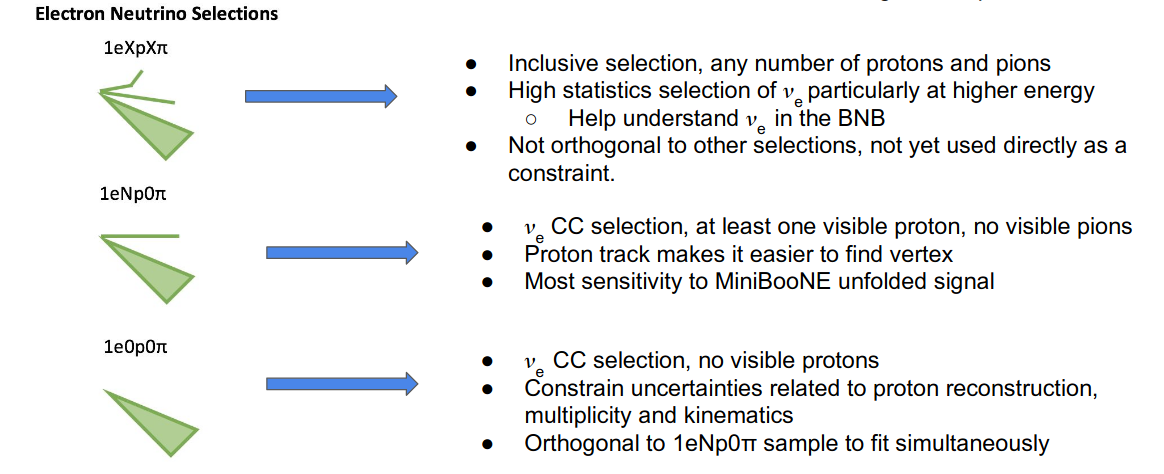
\includegraphics[width=0.85\textwidth]{introduction/nueselections.png}
%\caption{\label{fig:nueselections}Schematic of the three $\nu_e$ selection in this analysis, outlining the goals and strengths of each. In this work, the threshold for a visible proton at truth-level proton is 40 MeV of KE. $N$ refers to one or more and $X$ to any number of final state particles of a given category.}
%\end{center}
%\end{figure}


\begin{table}[ht]
\caption{\label{tab:selectionsNue} Schematic of the three $\nu_e$ selections, outlining the definition and goals of each. In this work, the threshold for a visible proton at truth-level proton is 40 MeV of KE. N refers to one or more and X to any number of final state particles of a given category.}
\centering
%\begin{tabular}{*{3}{ m{0.1\textwidth} }}
\begin{tabular}{ m{0.1\textwidth} | m{0.2\textwidth}  m{0.45\textwidth}  }
Channel & Description & Goal \\
\hline
 \begin{center}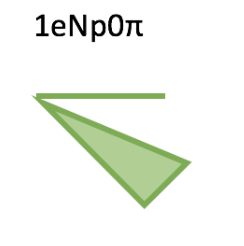
\includegraphics[width=0.1\textwidth]{introduction/1eNp}\end{center}& At least one visible proton and no visible pions & Most sensitive channel to MiniBooNE unfolded signal. The presence of a proton facilitates vertex finding.\\
\hline
 \begin{center}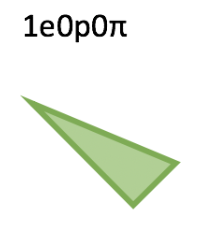
\includegraphics[width=0.1\textwidth]{introduction/1e0p}\end{center}& No visible protons and no visible pions & Constrain uncertainty related to proton reconstruction, multiplicity and kinematics for the 1$e$N$p$0$\pi$ channel.\\
\hline
\begin{center}\includegraphics[width=0.1\textwidth]{introduction/inclusive} \end{center} & Inclusive Selection: any number of protons and pions & Helpful to understand $\nu_e$ in the BNB: high statistic selection, especially at higher energies ($>$ 700 MeV). Not used as a constraint for other channels. \\
\hline
\end{tabular}
\label{tab:gt}
\end{table}


\par %\textbf{agnostic selection} 
In devising the selections presented above, we have deliberately chosen to not rely on cuts that make use of kinematic features of low-energy $\nu_e$ events. This allows the analysis to be agnostic to possible sources of new physics, and limits model dependence associated with assumptions on intrinsic $\nu_e$ interaction kinematics. Furthermore, an agnostic selection strategy allows to explore the kinematics of $\nu_e$ candidate events after their selection, for a full investigation of the origin of a potential anomaly. Implementing this choice requires the ability to fully leverage the information provided by the MicroBooNE LArTPC for $\nu_{\mu}-\nu_e$ and $e-\gamma$ separation. Significant progress has been made in developing tools for this goal, and will be described in subsequent sections. 




\subsection{Signal Model \textcolor{green}{David  ... (P.R. Elena) }}
\begin{comment}
%%%%%%% these are various parts that have been moved/modified
In order to benchmark the performance of the analysis it is valuable to have a signal model which can be used to assess the analysis' sensitivity.  This section describes the choice of model used for this purpose. It is important to stress that the signal model used serves the purpose of benchmarking the analysis' sensitivity, but the ultimate goal of our analysis remains to measure the rate of $\nu_e$ interactions in the BNB and report whether the observation is consistent or not with MicroBooNE's MC prediction.

\par Ultimately many signal models can be produced to test an analysis' sensitivity, each with its own set of important assumptions and caveats. % Or...
Ultimately any signal model used to test the analysis' sensitivity will carry a set of important assumptions and caveats. 
While reporting sensitivities for the MB-$\nu_e$ LEE model is useful, it is not exhaustive in being able to address MicroBooNE's ability to address MiniBooNE's anomaly. 
\end{comment}


\par  Many models can be devised to explain the MiniBooNE LEE as an excess of $\nu_e$ interactions, each model relying on a given (new) physics production mechanism and set of assumptions on the detector response. This section describes the signal model chosen by the collaboration to benchmark the sensitivity of all $\nu_e$ LEE analyses, including ours.  While a signal model is a useful tool, it is important to stress that any signal model carries a set of important assumptions and caveats, and that the ultimate goal of our analysis remains to measure the rate of $\nu_e$ interactions in the BNB, reporting whether the observation is consistent or not with MicroBooNE's MC prediction. Answering whether MicroBooNE's observation is consistent with the MiniBooNE LEE anomaly is beyond the scope of this work, and something not achievable without significant work for both MiniBooNE and MicroBooNE.
\begin{comment}
\par To test this analysis' sensitivity, a model explaining the MiniBooNE LEE  as an excess of $\nu_e$ interactions must be produced and used to generate simulated events in MicroBooNE. Many such models can be devised, each relying on a given (new) physics production mechanism and set of assumptions on detector response. 
\end{comment}

\par  The signal model used to generate simulated events in MicroBooNE and to compute the primary sensitivity quoted by this analysis  is the MiniBooNE-unfolded LEE model, referred to as \textbf{MB-$\nu_e$ LEE} model \cite{C,C2}. In this model, all excess LEE events are assumed to be due to $\nu_e$ interactions with a value of true energy obtained by unfolding from the reconstructed CCQE energy of MiniBooNE LEE events, as recorded by MiniBooNE's data. This procedure is performed by relying on MiniBooNE's energy smearing matrix. The resulting true neutrino energy distribution is shown in figure~\ref{fig:minibooneunfolded}. There are several limitations to this model worth observing, some technical, others conceptual. On a technical level, the model is composed of a binned event distribution, rather then a parametrized or analytic prediction of the expected $\nu_e$ spectrum. Additionally, no events below 200 MeV of true energy exist in this model. 
\begin{figure}[ht]
\begin{center}
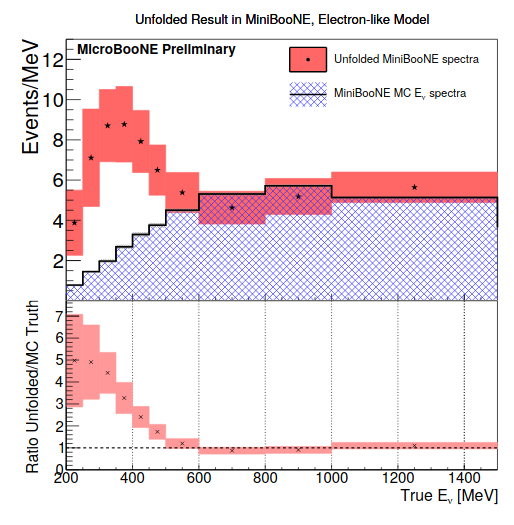
\includegraphics[width=0.45\textwidth]{introduction/unfoldedminiboone.png}
\caption{\label{fig:minibooneunfolded}MB-$\nu_e$ LEE signal model extracted from MiniBooNE's results.}
\end{center}
\end{figure}
Conceptual issues can be raised in association with the various assumptions made to generate the model. These include the strong reliance on MiniBooNE's simulation in order to unfold reconstructed to true neutrino energy, and the choice of such an unfolding procedure (performed as a function of $E_{\rm CCQE}$ rather then EM energy and $\theta$, for example).
It is especially important to note that the chosen model strongly favors the interpretation of MiniBooNE events as originating from very low energies (200-400 MeV) for which achieving high sensitivity may come at the cost of omitting a robust analysis at higher energies. This is something the analysis tries to avoid by developing an inclusive and kinematically unbiased analysis workflow. At the same time, we explore additional models for sensitivity calculations, most notably a 3+1 sterile-neutrino oscillation model. This is discussed in more detail in section~\ref{sec:sensitivity}.
\par Figure~\ref{fig:nuerate} shows the expected $\nu_e$ rate as a function of true neutrino energy split by final-state topology for the available MicroBooNE dataset of $10.1E20$ POT. % with a 10 cm FV. 
 MB-$\nu_e$ LEE signal events are shown in orange.
\begin{figure}[H] 
\begin{center}
    \begin{subfigure}[b]{0.45\textwidth}
    \centering
    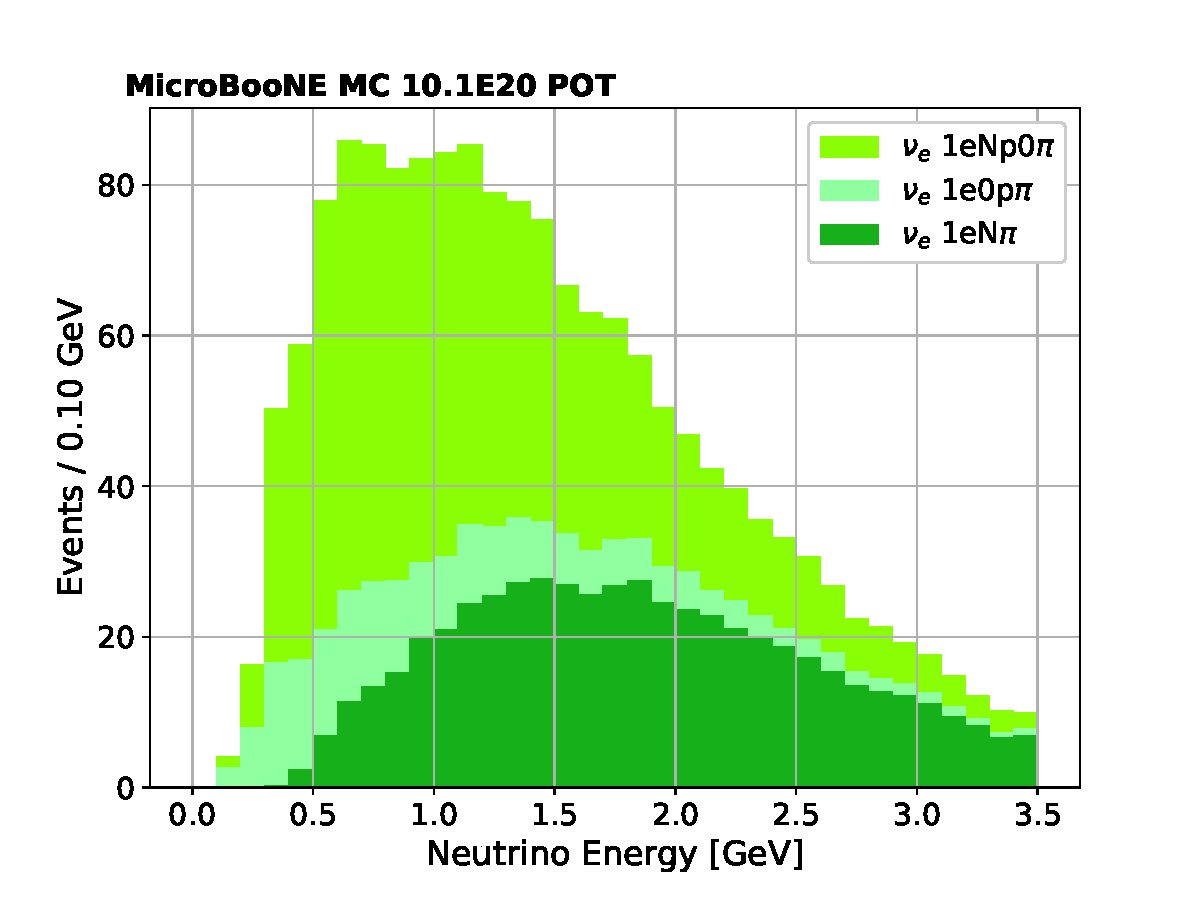
\includegraphics[width=1.00\textwidth]{introduction/nue_rate_MCC9.pdf}
    %\caption{\label{fig:nuerate:prediction}}
    \end{subfigure}
    \begin{subfigure}[b]{0.45\textwidth}
    \centering
    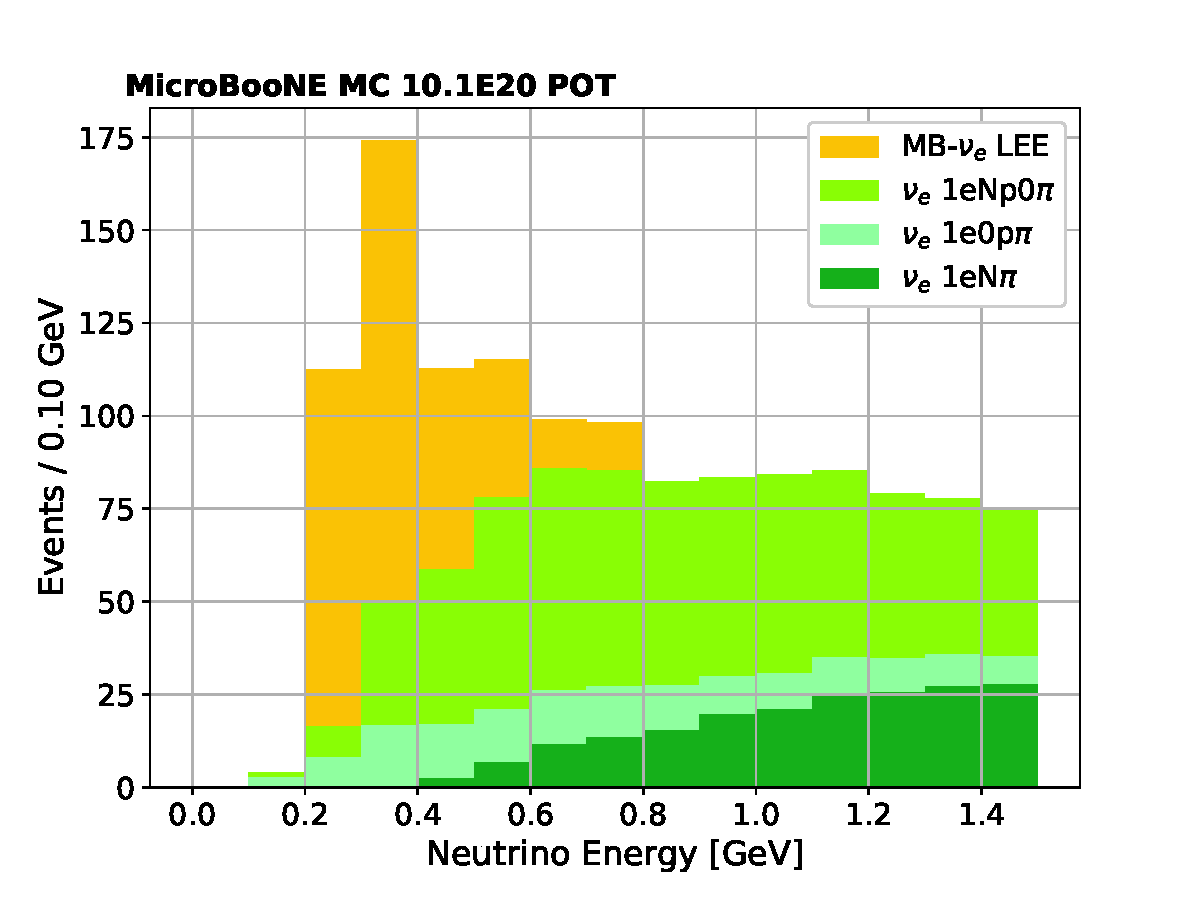
\includegraphics[width=1.00\textwidth]{introduction/nue_rate_MCC9_LEE.pdf}
    %\caption{\label{fig:nuerate:prediction:MC}}
    \end{subfigure}
\caption{\label{fig:nuerate}Expected $\nu_e$ rate in MicroBooNE for $10.1E20$ POT %in a 10-cm FV 
 subdivided by event topology (1$e$N$\pi$,1$e$N$p$0$\pi$, and 1$e$N$p$0$\pi$). The right-hand side figure highlights the low energy region with the unfolded $MB-\nu_e$ LEE signal prediction in orange.}
\end{center}
\end{figure}

\subsection{Goals of the $\nu_{\mu}$ Selection \textcolor{green}{David}}
\par For the purpose of this analysis, measurements of $\nu_{\mu}$ interactions are aimed at reducing modeling uncertainties for intrinsic $\nu_e$ events and backgrounds, with the goal of reducing systematic uncertainties in order to be able to claim the observation of new physics were a measurement of $\nu_e$ interactions differ significantly from the expected intrinsic rate. This section describes why such a data-driven constraint is needed and what are the choices which motivate the approach taken in this analysis.
\par Event reconstruction and $\nu_e$ identification are only one of the challenges in this analysis. In order to be able to make statements on whether the observed $\nu_e$ rate indicates a presence of new physics, a well understood prediction of the intrinsic $\nu_e$ expectation is needed. Uncertainties in the expected $\nu_e$ rate are associated to reconstruction efficiencies (detector effects) as well as modeling uncertainties in both the $\nu_e$ flux prediction and neutrino-argon cross-section modeling. Here we focus on describing the strategy employed to deal with flux and cross-section uncertainties. Modeling uncertainties in the expected rate of $\nu_e$ interaction are large, and can limit the ability to associate a $\nu_e$ measurement with potential new physics if not constrained through additional measurements. Flux uncertainties for $\nu_e$ are $\mathcal{O}$(10\%) above 800 MeV and grow to 40\% at 200 MeV. Cross-section uncertainties are also large, a consequence of a lack of measurements of $\nu$-Ar cross-sections, particularly at low energy, and the complex modeling of neutrino interactions on a heavy target such as argon. Combining all effects, the uncertainty on the $\nu_e$ interaction rate in the few-hundred MeV energy range in MicroBooNE's could be as high as 100\%.
\par To reduce modeling uncertainties on the expected rate of $\nu_e$ interactions, data-driven constraints are required. These can be performed through measurements of $\nu_{\mu}$ interactions subject to the same uncertainties. In order to constrain flux uncertainties, we rely on the fact that $\nu_e$ and $\nu_{\mu}$ intrinsic to the beam are produced by the decay of the same parent $\pi$ and $K$ flux. Similarly for uncertainties on neutrino interaction modeling, we rely on the common charged-current interaction mode $\nu_{l} + Ar \rightarrow l + X$ for both $\nu_{\mu}$ and $\nu_e$ interactions to constrain interaction uncertainties. 
\par The complexity of $\nu$-Ar interactions and of hadronic interactions in the beamline mean that many different handles and measurements of $\nu_{\mu}$ interactions can play a role in constraining different uncertainties. As examples, measurement of CC and NC $\pi^0$ production constrain resonant interactions and thus $\pi^0$ backgrounds to the $\nu_e$ selection, and measurements of high-energy $\nu_{\mu}$ interactions can help constrain the kaon flux in the beam, which contributes substantially to the production of intrinsic $\nu_e$s. Likewise, measurements of low-energy $\nu_{\mu}$s can help constrain poorly understood $\nu$-Ar interaction models in the few-hundred MeV energy regime, a critical requirement for this analysis. The neutrino identification work developed for this analysis, referred to as \emph{SliceID} and described in section~\ref{sec:sliceID}, is a highly efficient and topology agnostic selection that enables a vast program of $\nu_{\mu}$ measurements, allowing for flexibility in selecting topologies that may have the strongest constraining power and thus most benefit the $\nu_e$ analysis. At the current time, as described in the remainder of this section and in section~\ref{sec:systematics}, the emphasis is on the measurement of low-energy $\nu_{\mu}$ interactions with the goal of constraining the large uncertainties in low-energy $\nu_e$ events which significantly impact the analysis.
\par To further motivate the need for low energy $\nu_{\mu}$ interactions, we describe two important ways in which such a dataset can benefit the reduction of modeling uncertainties for $\nu_e$ interactions. Figure~\ref{fig:numuconstraint:flux} shows the flux correlation for $\nu_{\mu}$ (bottom left) and $\nu_e$ (top right) interactions. Red (blue) areas show large (anti-)correlation. The top-left or bottom-right quadrants show the strength of correlations between the two flavors. For $\nu_e$ energies below 1 GeV, correlations are strongest with $\nu_{\mu}$ interactions at low energy. Figure~\ref{fig:numuconstraint:xsec} shows different cross-section curves for $\nu_{\mu}$ and $\nu_e$ interactions. The dashed and solid curves represent the CCQE cross-section used in MCC8 vs. MCC9 respectively. Below 400 MeV, the difference in event rates for different models is larger then 100\%. The large differences between these curves, particularly at low energy, indicate the strong need to constrain cross-section uncertainties with MicroBooNE's own data. 
\begin{figure}[ht] 
\begin{center}
    \begin{subfigure}[b]{0.42\textwidth}
    \centering
    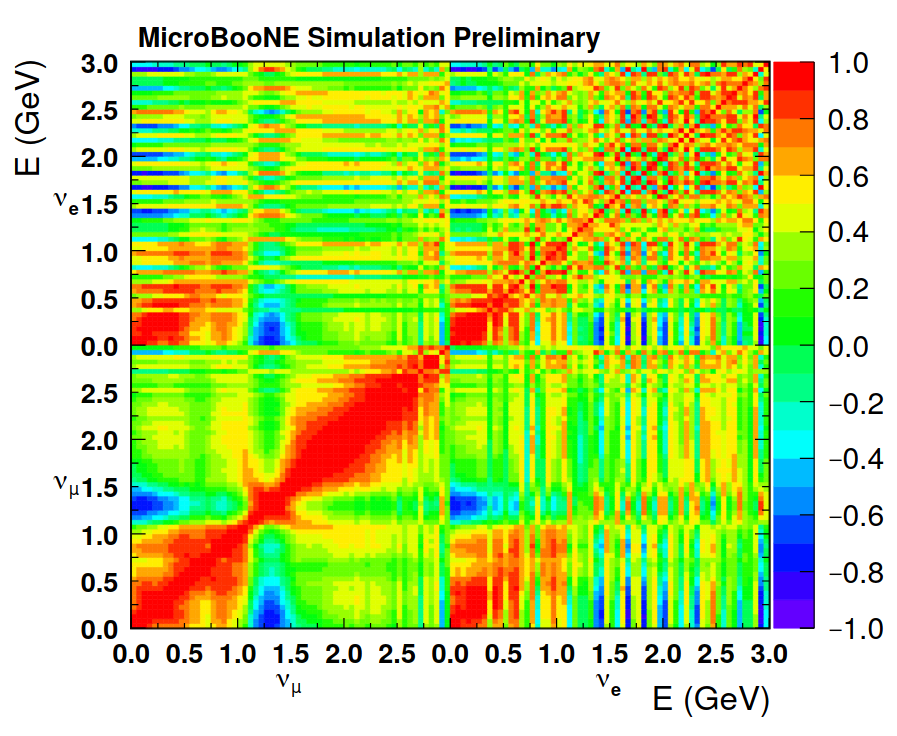
\includegraphics[width=1.00\textwidth]{introduction/fluxcorrelation.png}
    \caption{\label{fig:numuconstraint:flux}$\nu_{\mu}$-$\nu_e$flux correlation matrix}
    \end{subfigure}
    \begin{subfigure}[b]{0.3\textwidth}
    \centering
    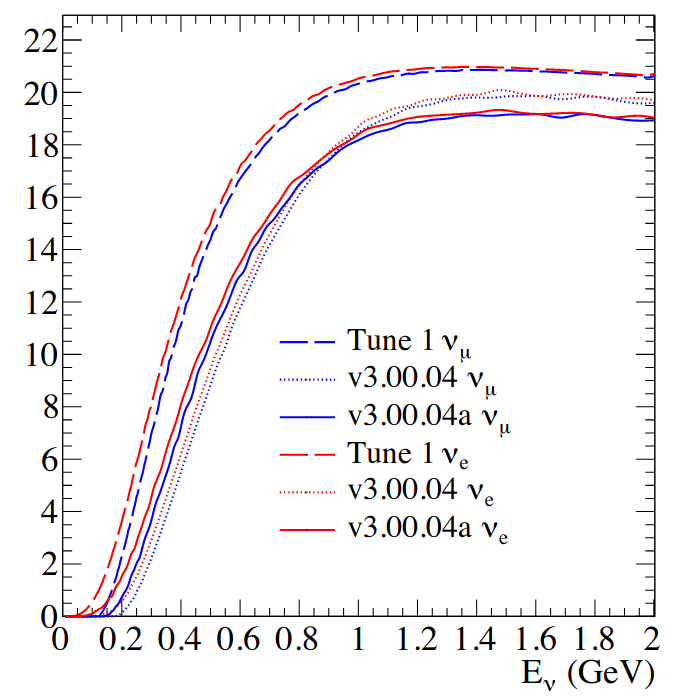
\includegraphics[width=1.00\textwidth]{introduction/xsec_mcc8_mcc9.png}
    \caption{\label{fig:numuconstraint:xsec}different xsec models for CC interactions.}
    \end{subfigure}
\caption{\label{fig:numuconstraint}}
\end{center}
\end{figure}

\subsection{Systematics  \textcolor{green}{David}}
\par This section gives a brief overview of how detector and modeling uncertainties are accounted for in the analysis. The estimation of systematics is performed in section~\ref{sec:systematics}.
\par \noindent \textbf{Detector Systematics}: Detector modeling in MicroBooNE has undergone significant updates in the past year, in part as a result of the large impact that detector systematics have had on 2018 analyses (\textcolor{red}{cite CCpi0,CCincl}). Detector effects with significant impact on the analysis can be broken up into three main categories:
\begin{itemize}
    \item wire-response modeling: the response of MicroBooNE's electronics to drifting charge is a complex subject described in three past publications~\cite{bib:noise,bib:SP1,bib:SP2}. The work of these papers in improving the understanding and modeling of noise and field-response effects has been implemented in the current detector simulation and is expected to lead to a reduction in what for MCC8 analysis comprised the largest detector uncertainty.
    \item Space-Charge modeling: MicroBooNE's space-charge model has changed significantly since 2018, moving from a calculation-based~\cite{bib:SCETN} implementation of electric field distortions to a data-driven E-field map implemented in simulation and reconstruction. Due to the large position distortions (and, though smaller, charge distortions) SCE can significantly impact an analysis through the determination  of fiducial boundaries, tracking and energy resolution.
    \item Scintillation light modeling: MicroBooNE's model of scintillation light production has not changed significantly since the beginning of data-taking, and has known limitations. Of particular importance to this analysis, which aims to use a dataset spanning four years, is the known and significant time-dependent variation of MicroBooNE's light response. This analysis takes several steps to correct for, and mitigate the impact that light mismodeling can have on the analysis. Triggering on low-energy signal $\nu_e$ events, and cosmic-rejection are particularly sensitive to scintillation light detector effects.
\end{itemize}{}
An additional detector effects that needs to be accounted for are ion Recombination which impacts the detector's calorimetric response. Tailored studies and proton samples are being developed to assess ion recombination modeling accuracy in MCC9.
\par \noindent \textbf{Flux and Cross-Section Modeling} Uncertainties in flux and cross-section modeling are treated through a \emph{multi-sim} approach, where underlying parameters that are input to the modeling are varied in a correlated way. Flux uncertainties are taken from the MiniBooNE BNB flux simulation adapted to MicroBooNE~\cite{bib:fluxmcc9}, while $\nu$ interaction uncertainties are handled within the \texttt{GENIE} reweighting package, as described in~\cite{bib:geniesupportnote}. We note that the \texttt{GENIE} event reweighting infrastructure is still in development and likely to be updated or further expanded on in the future. Finally, uncertainties associated with pion and proton re-interactions in argon were unavailable when this version of the Tech Note was produced and not included at this stage.

\subsection{Sensitivity Calculation  \textcolor{red}{Nico/Maya}}
\subsection{Money Plots and Takeaways \textcolor{red}{Elena/David/ Group discussion}}

\newpage

\section{Overview of Neutrino Identification: Pandora SliceID}
%\subsection{Event Slicing and Cosmic Removal in Pandora}

The work presented in this note relies on the Pandora approach for event reconstruction~\cite{bib:pandoraub}. The scope of Pandora is to do the low-level pattern-recognition step of the reconstruction, i.e. group hits into clusters, clusters into particles and particles into hierarchies. This section describes how Pandora's pattern-recognition output is combined with scintillation light information to isolate possible candidate neutrino interactions in MicroBooNE events, a process illustrates in the three images of figure~\ref{fig:sliceid}. 

\begin{figure}[ht] 
\begin{center}
    \begin{subfigure}[b]{0.7\textwidth}
    \centering
    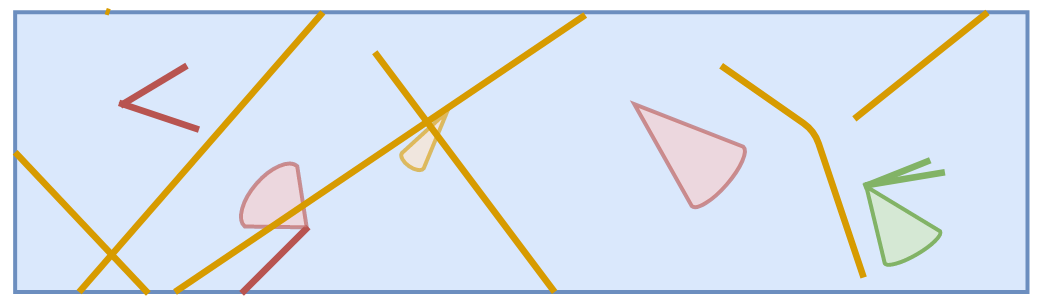
\includegraphics[width=1.00\textwidth]{NuId-Ch2/Images/slice00.png}
    \caption{\label{fig:slcieid:00} Typical event with multiple interactions isolated by Pandora in \emph{slices}.}
    \end{subfigure}
    \begin{subfigure}[b]{0.7\textwidth}
    \centering
    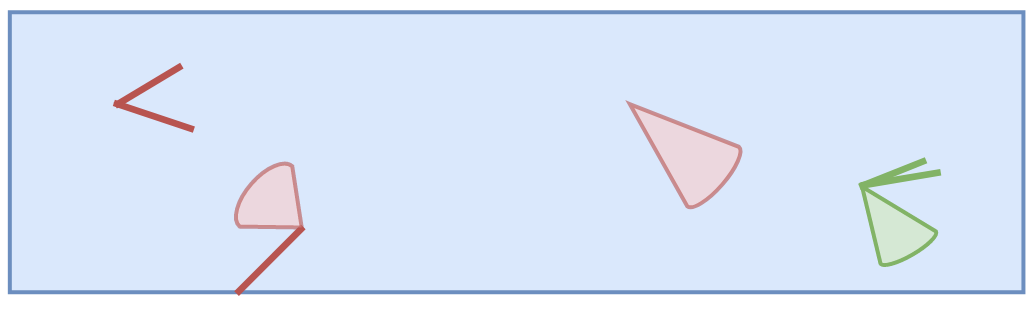
\includegraphics[width=1.00\textwidth]{NuId-Ch2/Images/slice01.png}
    \caption{\label{fig:slcieid:01} Event after the removal of \emph{obvious cosmics} tagged geometrically by Pandora.}
    \end{subfigure}
    \begin{subfigure}[b]{0.7\textwidth}
    \centering
    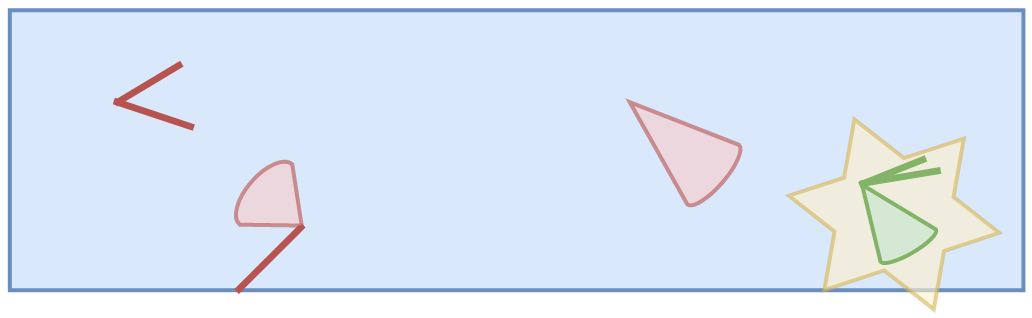
\includegraphics[width=1.00\textwidth]{NuId-Ch2/Images/slice02.png}
    \caption{\label{fig:slcieid:01} Implementation of the \texttt{SiceID} tool to isolate possible candidate $\nu$ interactions.}
    \end{subfigure}
\caption{\label{fig:sliceid} Succession of steps in cosmic removal performed using Pandora's topological pattern recognition combined with scintillation light information through the \texttt{SliceID} tool.}
\end{center}
\end{figure}

\subsection{Slicing \textcolor{green}{Wouter ... P.R. Elena}}
The creation of a ``slice" is the first step of the Pandora processing. A slice \textcolor{blue}{is a collection of distinct reconstructed particles which belong to the same interaction (such as a cosmic muon and its Michel electron, or the muon and proton in a 1$\mu$1$p$ neutrino interaction) \st{is a combination of hits on the three different planes which are topological distinct:  it is assumed that different slices correspond to a distinct group of activity in the TPC}}. To produce slices, the Pandora Cosmic Pattern Recognition is first run over all hits, aiming to construct muon tracks and associated $\delta$-rays and Michel electrons under the cosmic hypothesis (fig.~\ref{fig:sliceid:00}). At this stage, obvious cosmic activity (through-going or out-of-time muons) is tagged using geometric information. The obvious cosmic tagged hits are discarded (fig.~\ref{fig:sliceid:01}); the filtered hit collection is used as input to the Pandora Consolidated Pattern Recognition which reconstruct slices under the neutrino hypothesis. Each slice is now reconstructed both under the cosmic hypothesis and the neutrino hypothesis. A typical event contains approximately 5 slices. 

\subsubsection{Clustering and Vertex Finding \textcolor{green}{Wouter}} 
Pandora computes the 2D clustering on the hits in each slice and in each plane separately. Then, a number of 3D candidate vertices is created by finding positions that project down on to the ends of the available 2D clusters. All of the possible candidates are fed into the support vector machine (SVM) vertex selection, and the most appropriate one is chosen. This 3D vertex is used to split any existing clusters that straddle the vertex. Then, the cluster matching algorithms are run, where the clusters are compared between views and modified to improve the matching.

\subsection{SliceID : Cosmic Removal through topology and scintillation-light \textcolor{green}{Wouter}}
\label{sec:sliceID:SliceID}
\par After the Pandora pattern-recognition algorithm suite has isolated individual interactions into reconstructed \emph{slices} and removed those that are either through-going or out-of-time, the remaining task is to identify which (if any) slice is associated to a neutrino interaction. This is done by relying on scintillation light information to reject slices incompatible with light recorded in-time with the beam. Additionally, topological cuts aimed at rejecting stopping-muon events which enter the TPC are used. The SliceID is at the core of all neutrino selections performed in this analysis, and serves as the first, common step in the analysis, responsible for the majority of cosmic-rejection.
\\
\par We have three handles that we use to distinguish between neutrino and cosmic-ray slices.
\begin{enumerate}
    \item Simple optical pre-selection cuts - is the slice totally inconsistent with the beam flash?
    \item Topological score - to what extent does the slice look like a neutrino interaction in the TPC?
    \item Flash-matching score - to what extent does our flash-hypothesis for this slice match the beam flash?
\end{enumerate}
To select the neutrino slice, or reject the event at this stage, the following procedure is followed:
\begin{itemize}
    \item Insist that there is a beam-triggered flash in the beam window.
    \item Only consider slices that pass the optical pre-selection cuts.
    \item If the slice with the largest topological score in the event remains, then select it as the neutrino.
    \item If not, then choose the remaining slice with the largest flash-matching score.
\end{itemize}
Further details on the \texttt{SliceID} tool are available in DocDB 23854 and 22519. Additional documentation for this tool is in preparation.

The performance of the SliceID for electron neutrino simulated events is given in~\cref{fig:sliceid}.

\begin{figure}[H]
    \centering
    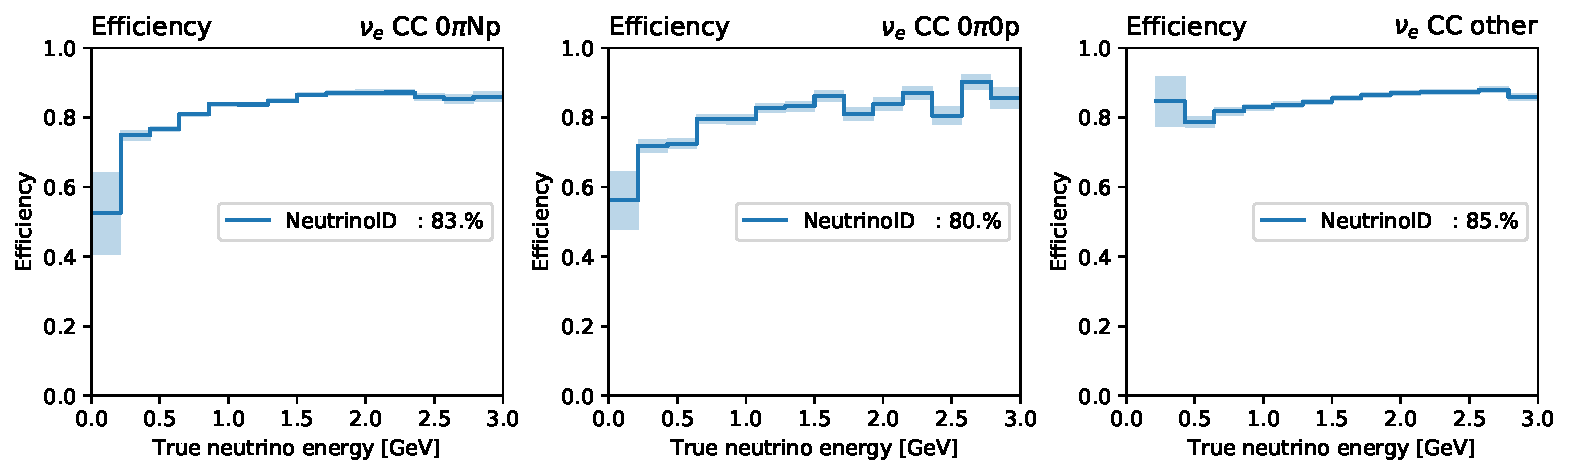
\includegraphics[width=\textwidth]{NuId-Ch2/Images/efficiency_cat_0.pdf}
    \caption{The performance of the SliceID in function of the true neutrino energy for the channel with protons (left), the channel without vertex activity (middle) and events with pions in the final state (right).}
    \label{fig:sliceid}
\end{figure}



\subsection{CRT Veto and Distance Tagger \textcolor{green}{Elena}}
\label{sec:sliceID:CRT}
Contrary to  $\nu_\mu$ interactions and cosmic rays, the charged particles associated to $\nu_e$ interactions are unlikely to deposit energy in the Cosmic Ray Tagger (CRT). Building upon this discriminating factor, the CRT Veto and CRT Distance Tagger are preselection tools which leverage the additional CRT information available for Run 3+ data.
When used, these CRT tools are applied at the pre-selection stage in the following order: CRT Veto, SliceID, CRT Distance Tagger. The CRT tools are especially impactful for the 1e0p channel, where discrimination handles based on the proton PID are obviously missing. \\


\emph{CRT Veto.} %On average, only one in six events passing the MicroBooNE common optical filter is associated to beam-induced activity. The remaining events are triggered by activity that originates outside the TPC: either external beam induced activity or cosmic rays. %Given the $\mathcal{O}(10)$ cosmic ray muons in each drift window, this equates to a starting signal-to-background of $\sim 1 : 60$.
%The CRT Veto looks at CRT activity in time with the beam window. 
The CRT veto looks for a time coincidence between the scintillation light recorded in time with the 1.6 $\mu$s beam-spill (beam-flash) and a CRT hit: if a CRT hit occurs within a 1 $\mu s$ of the beam flash, the event is rejected. For this coincidence, only CRT hits with PE $>$ 100 pe are considered; we do not apply a constraint on the position of the flash nor on the position of the CRT hit. 
The rejection power and efficiency of the CRT veto are calculated using the BNB external and the $\nu_e$ overlay samples, respectively. The BNB external passing rate is $\sim$59\%,  and the $\nu_e$ efficiency greater than $\sim$94\% for all electron neutrino energies, raising at low energies. \\


\emph{CRT Distance Tagger.} 
The CRT Distance Tagger tool builds upon the standard pandora neutrino vertex reconstruction and the CRT tagging of TPC tracks. A TPC track is tagged with a CRT hit association if the track projection onto a CRT panel and a CRT hit are close in space. 
To perform this association, the track projection to the CRT is calculated under the hypothesis that the associated particle crossed the TPC at the time registered by the CRT hit under consideration; more details on the CRT hit to TPC track match are available in \cite{bib:CRTPresel_Technote}.  The CRT Distance Tagger checks the minimum distance between the reconstructed neutrino vertex and each track tagged with a CRT hit. If the minimum distance is less than 14 cm, the event is rejected. An example event tagged by this cut is shown in Figure~\ref{fig:crtdist00}.  For the CRT Distance Tagger, the BNB external passing rate is $\sim$81\%,  and the $\nu_e$ efficiency greater than $\sim$96\% for all electron neutrino energies, raising at low energies. \\
 
\begin{figure}[h!]
\centering
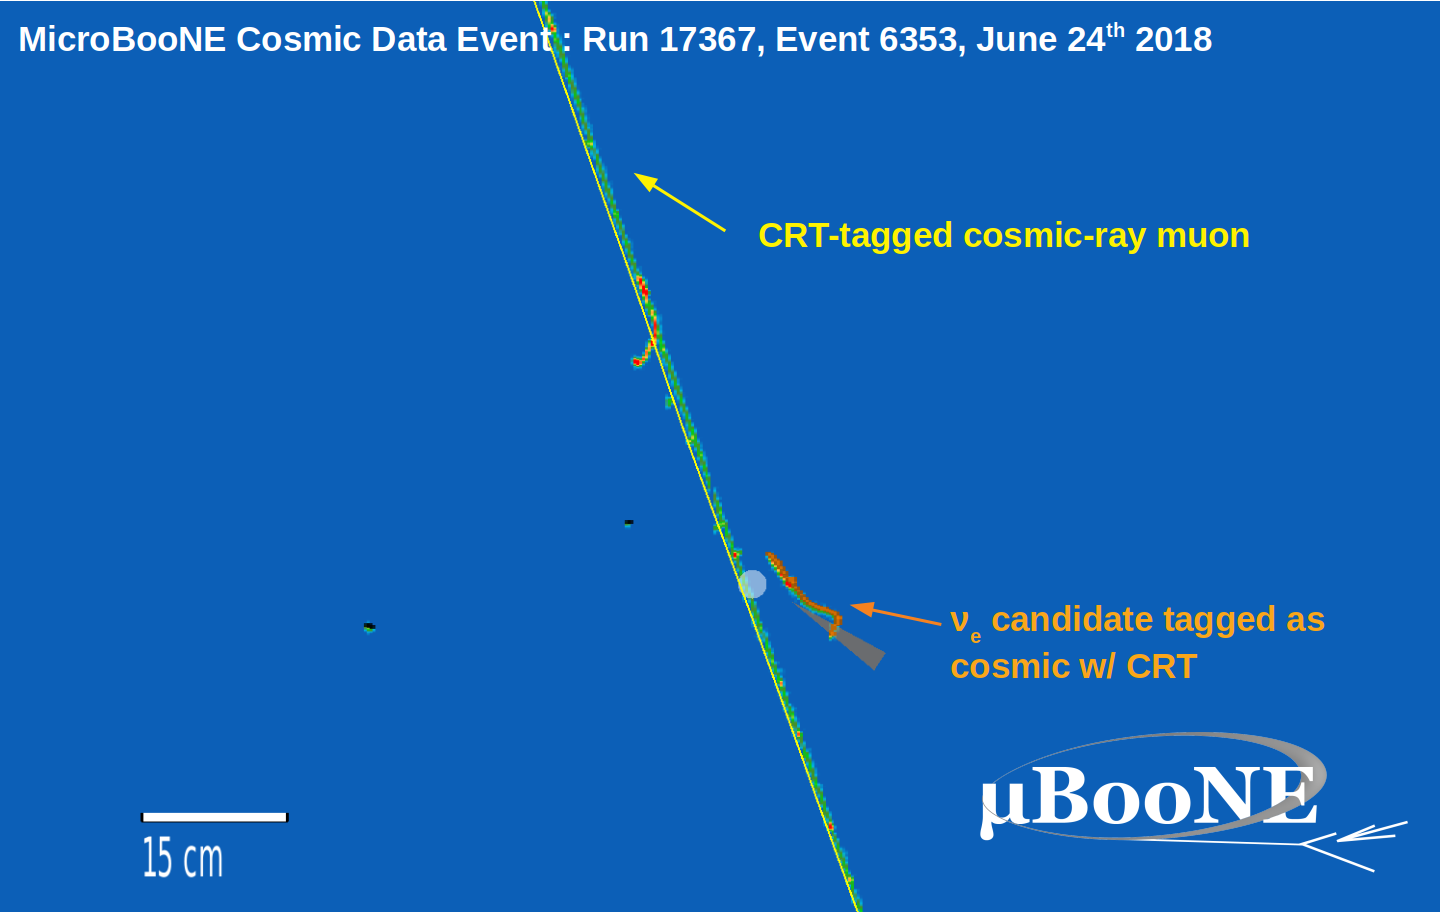
\includegraphics[width=0.4\textwidth]{NuId-Ch2/Images/crttagger_01.png}
\caption{Example $\nu_e$ candidate tagged as cosmic thanks to the CRT distance tagger. From the event one can see that the reconstructed EM shower is associated to EM activity associated to the incoming muon.}
\label{fig:crtdist00}
\end{figure}

An overview of the impact of the CRT on cosmic rejection can be seen in Figure~\ref{fig:crt} where the beam-time distribution for the $8E18$ POT Run 3 open dataset is shown after SliceID (left), and after SliceID and CRT cosmic-tagging tools (both CRT veto and distance tagger) have been applied (right), with EXT backgrounds dropping by more than a factor of 3.
Further details and a preliminary study of the CRT  impact on an electron neutrino preselection can be found in \cite{bib:CRTPresel_Technote}. 

\begin{figure}[ht] 
\begin{center}
    \begin{subfigure}[b]{0.4\textwidth}
    \centering
    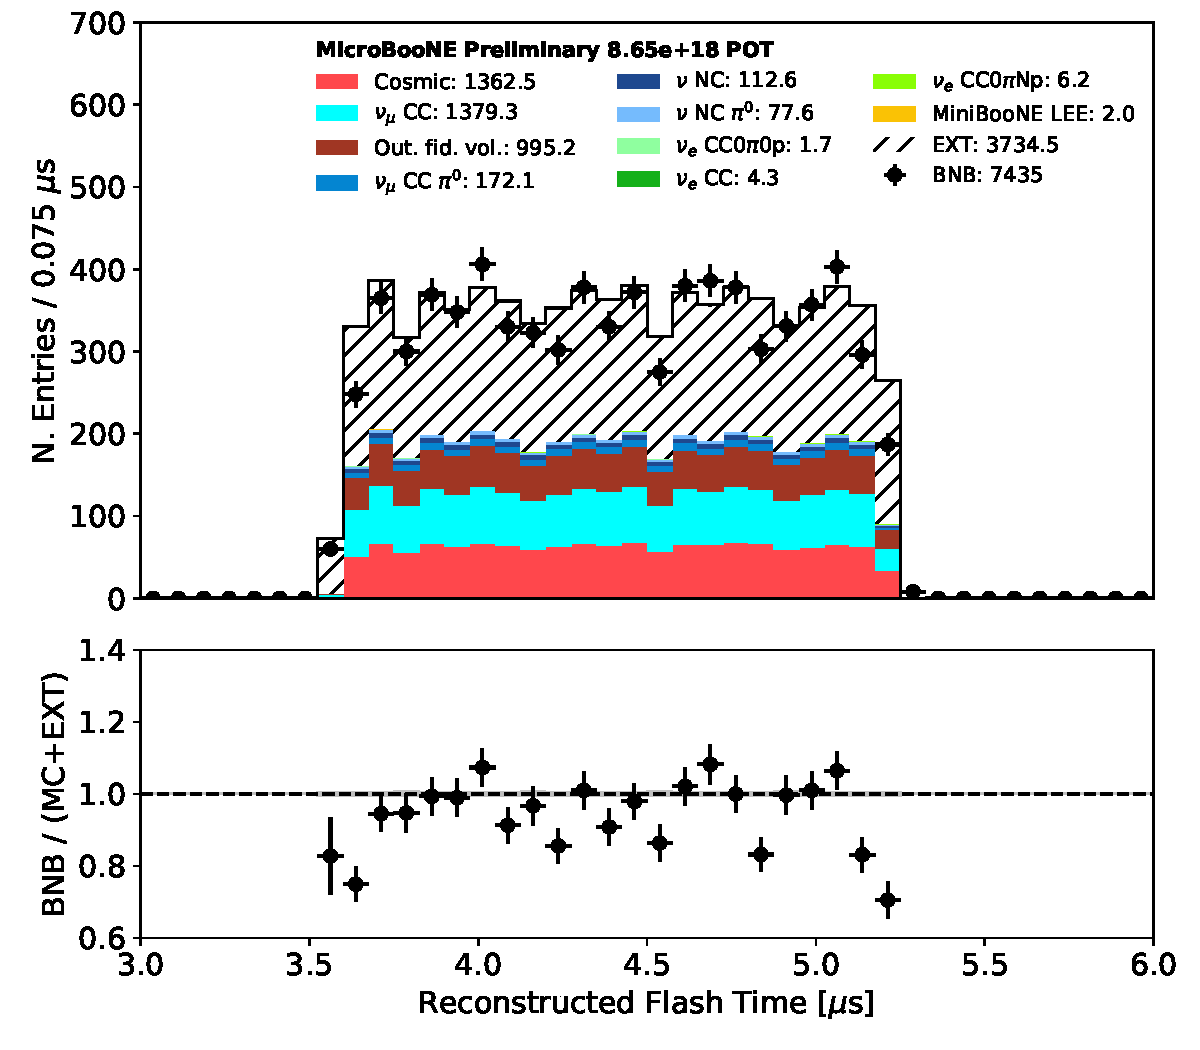
\includegraphics[width=1.00\textwidth]{NuId-Ch2/Images/flash_time_01152020.pdf}
    \caption{\label{fig:crt:pre} no CRT tools.}
    \end{subfigure}
    \begin{subfigure}[b]{0.4\textwidth}
    \centering
    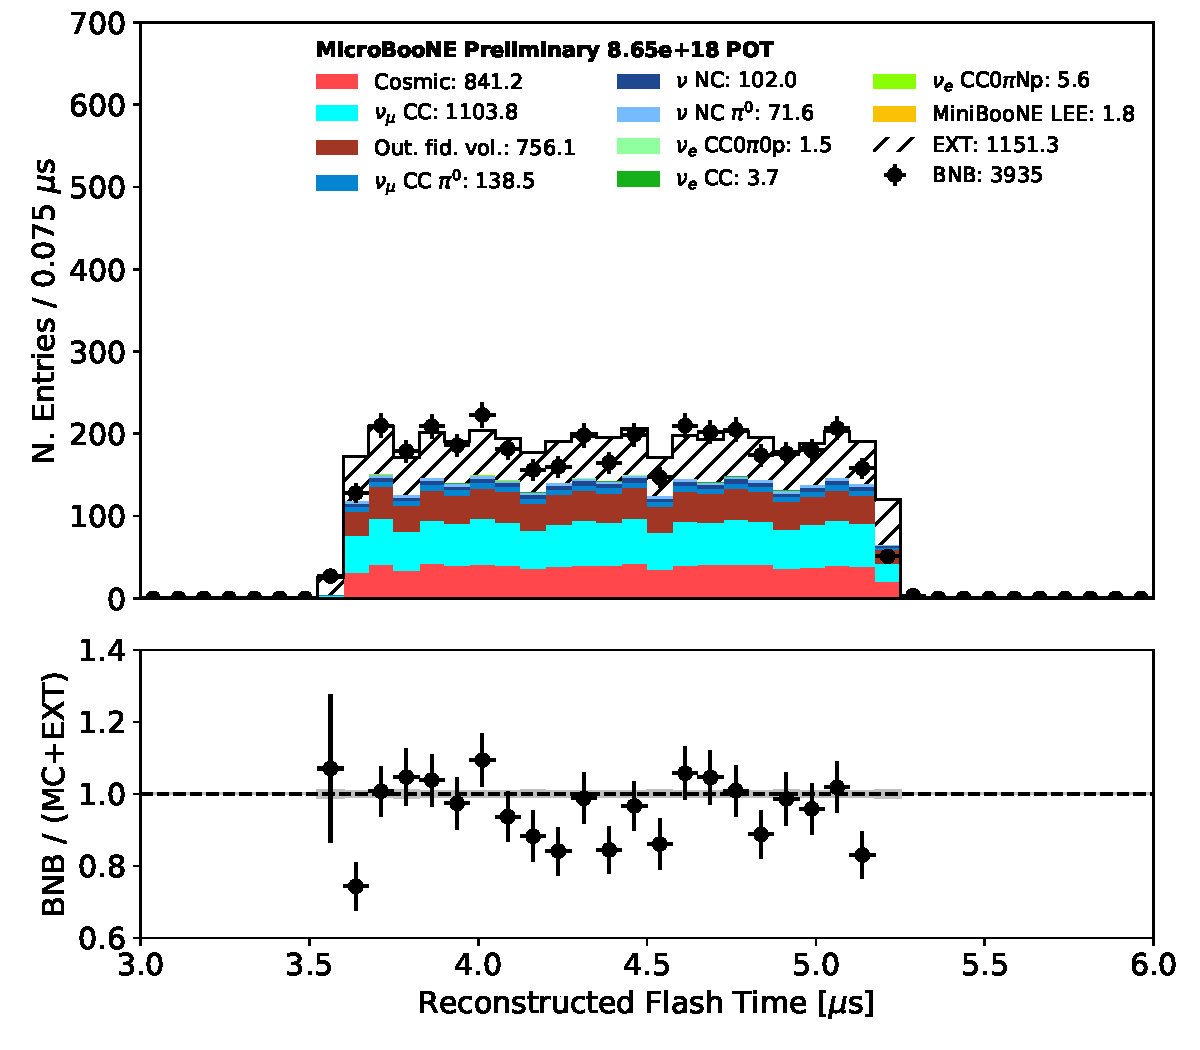
\includegraphics[width=1.00\textwidth]{NuId-Ch2/Images/flash_time_01152020_CRT.pdf}
    \caption{\label{fig:crt:post} with CRT tools.}
    \end{subfigure}
\caption{\label{fig:crt} Beam timing distribution before (left) and after (right) CRT tools have been applied. The EXT contribution is reduced by over a factor of three.}
\end{center}
\end{figure}



\newpage

\section{Neutrino Event Reconstruction}

\subsection{Track and Shower Reconstruction \textcolor{green}{Giuseppe}}
\label{sec:tkshreco}
The output of Pandora~\cite{bib:pandoraub} is organized in a hierarchy of reconstructed Particle Flow Particles (``PFParticles''), which describes the particle content in an observed event as a parent-daughter relationship chain. Final state PFParticles are 3D objects matching clusters of hits in at least two different planes.
Pandora classifies PFParticles as track-like or shower-like base on a Support Vector Machine (SVM) algorithm~\cite{bib:tkshsvm}, producing a score with values between 0 (shower-like) and 1 (track-like).

Pandora processes track-like PFParticles with a sliding linear fit procedure (described in~\cite{bib:pandoraub}) that returns the 3D position and direction at each point along the trajectory (where each point corresponds to a 2D hit). For each point the d$Q$/d$x$ and distance from the track-start are recorded using MicroBooNE's Calorimetry module. This procedure allows to accurately measure d$x$, including small deflections due to the particle's trajectory and SCE offsets, and d$Q$, by incorporating MicroBooNE's full position- and field-dependent relative and absolute charge calibration. From d$Q$/d$x$, d$E$/d$x$ is calculated assuming a fixed recombination correction assuming 2.1 MeV/cm energy loss, but accounting for local variations in the electric field.

We evaluate the energy and 3D direction of shower-like PFParticles with the same algorithm used for the $\pi^0$ reconstruction paper~\cite{bib:pi0reco}. The energy reconstruction accounts for various detector effects, including gain and recombination; corrections for reconstruction effects (hit threshold and imperfect clustering) will be described in Sec.~\ref{sec:ereco}. We also fit showers using a Kalman filter-based procedure~\cite{bib:shrtrackfitter} which aims at identifying the main trunk of the shower by rejecting hits that are longitudinally or transversely displaced from it; the output of this fit is a track object so that the calorimetric tools described above become available for showers as well.

By default, Pandora separates showers and tracks with a cut on the SVM score at 0.5; however, as will be described in later sections, in many cases we choose different cut values, i.e. tighter shower definition for the $\nu_e$ selection and looser for the pi0 control region.

\par The Efficiency of Pandora's reconstruction on $\nu_e$ interactions is evaluated in figure~\ref{fig:nuereco:eff} as a function of true neutrino energy and shows the efficiency for correctly identifying $\nu_e$s in the event in black, and the efficiency for reconstructing $\nu_e$ interactions with a final-state EM shower in blue. The efficiency has a sharp upturn between 100 and 200 MeV, especially in the case when an EM shower is required, and levels off at 80\% and 60\% respectively for the two curves. 
\par At this stage in the analysis, the good efficiency for reconstructing $\nu_e$ events is offset by the very low signal-to-background for $\nu_e$ events in MicroBooNE's data, a consequence of the very small $\nu_e$ content of the beam. With no additional requirement on the reconstructed neutrino, the purity for $\nu_e$ interactions is 0.12\%. After imposing a requirement of one reconstructed shower, the purity grows by almost an order of magnitude, to 1\%. The $\nu$ background composition also changes significantly, with $\pi^0$ backgrounds moving from 14\% to 48\% of all backgrounds.

\begin{figure}[ht] 
\begin{center}
    \begin{subfigure}[b]{0.3\textwidth}
    \centering
    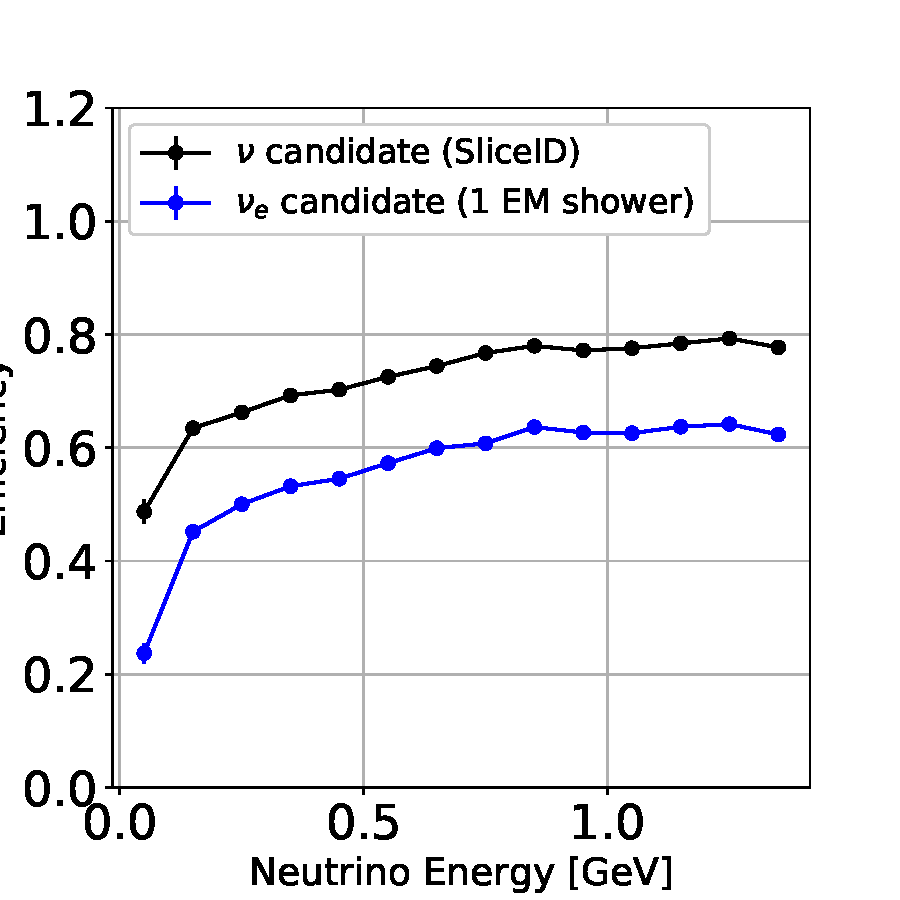
\includegraphics[width=1.00\textwidth]{nureco/nureco_RUN1.pdf}
    \caption{\label{fig:nuereco:eff} $\nu_e$ reco eff.}
    \end{subfigure}
    \begin{subfigure}[b]{0.31\textwidth}
    \centering
    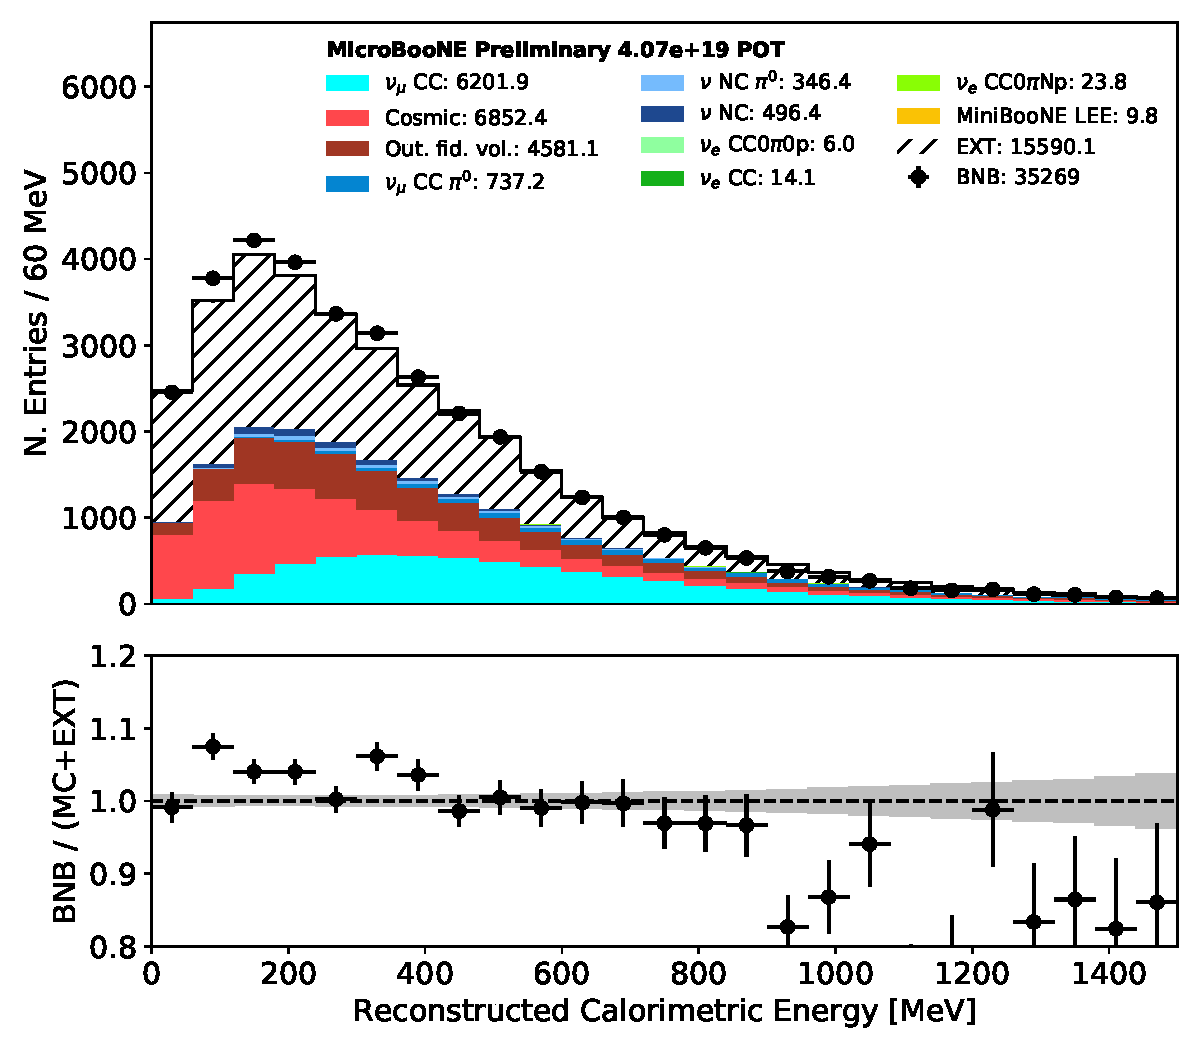
\includegraphics[width=1.00\textwidth]{nureco/NeutrinoEnergy2_01152020.pdf}
    \caption{after SliceID}
    \end{subfigure}
    \begin{subfigure}[b]{0.31\textwidth}
    \centering
    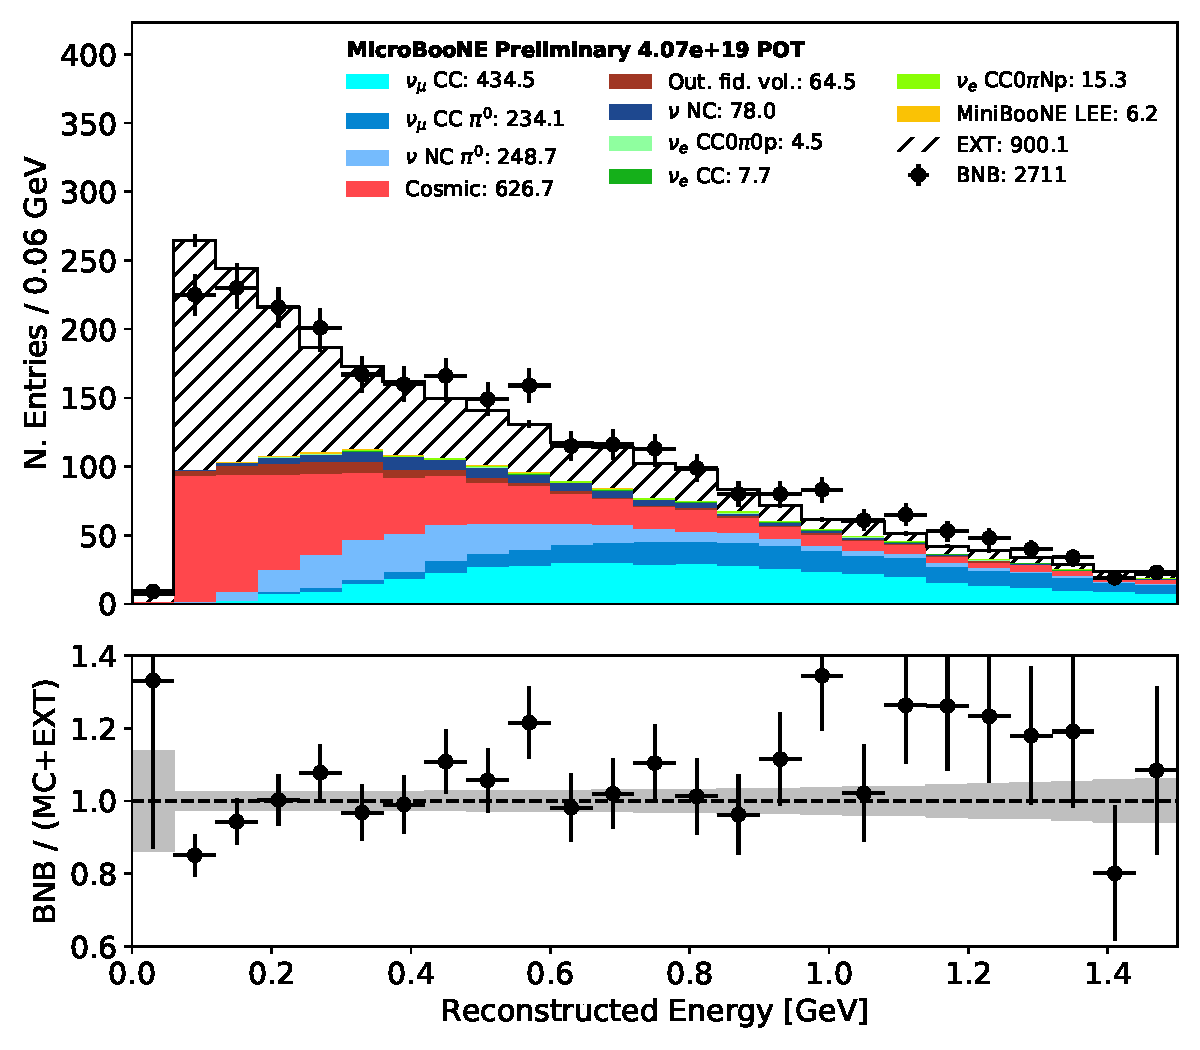
\includegraphics[width=1.00\textwidth]{nureco/reco_e_01152020.pdf}
    \caption{\label{fig:egammasep:dedx} after shower requirement}
    \end{subfigure}
\caption{\label{fig:nuereco}}
\end{center}
\end{figure}

\par The next step in the analysis demands the development of a selection capable of isolating $\nu_e$ interactions rejecting the two order of magnitude larger background rates from $\nu_{\mu}$ neutrinos. This selection will make use of PID and topological information described in the next sections. The strong level of background rejection needed to isolate signal events will inevitably lead to a lower selection efficiency.

\subsection{Particle Identification \textcolor{green}{Nico}}
% GC: this part is now in the previous subsection
%In the neutrino slice, every PFParticle is reconstructed in three different ways:
%\begin{itemize}
%    \item Track, using the standard Pandora Track reconstruction
%    \item Shower, using the standard Pandora Shower reconstruction (is there any modification on top of this?)
%    \item Track-fitted shower, using a dedicated track fitting tool which aims at identifying the main branch of %the shower and fit it as a track. As a result, all the tools developed for the track become available for the %tracks too. For example, for each track-fitted shower, a recob::track and a anab::calorimetry objects are available.
%\end{itemize}
Particle identification is performed with different tools depending the type of candidate a given PFParticle has been selected as.
If the PFParticle has been selected as a muon or proton candidate, so as a track-like object, the identification is performed using the Calorimetry Likelihood tool, which results in the variable Log Likelihood Ratio PID  (section~\ref{subsec:loglikelihoodpid}).
If the PFParticle has been selected as an electron or photon candidate, the identification is performed using several variables described in \ref{subsec:egammaspearation}.

It is noteworthy that this particle identification consists of one or multiple variables, available for the specific PFParticle, that may or may not depend on the rest of the slice. 
For example, the shower dE/dx depends only on the PFParticle itself, whereas the track-shower separation relies also on additional objects identified in the slice.

The value of the cuts applied on these variables depend not only on the general level of efficiency and mis-identification one may want to achieve in distinguishing two kind of particles (electrons from photons, for example), but also on the mixture of backgrounds, which eventually depends on the specific selection the analyser is performing.

\subsubsection{Log Likelihood Ratio Particle ID \textcolor{red}{Nico}}
\label{subsec:loglikelihoodpid}

For track-like particles, the particle identification is performed looking at the profile of the deposited charge per unit length ($dE/dx$).
The scope of particle identification is to tell the type of particle a certain track was originated from.
For what concerns this analysis, it has been decided to limit the problem to a binary classification problem, distinguishing protons from muons.
In fact, kaons are produced rarely in neutrino interactions at this energy, whereas pions are very difficult to distinguish from muons, given the very similar mass and the current resolution of the detector.
Additional information, such as possible hadronic reinteractions or Michel electrons, can be powerful to perform particle identification.
No additional information is used in this analysis, as we believe the reconstruction is not precise enough to tag such reinteractions.

The expected distribution of the $dE/dx$ is modeled for each particle type and for each plane, as a function of two variables: the residual range ($rr$), and the pitch.
\[ p(dE/dx | \text{type}, \text{plane}, \text{rr}, \text{pitch}) \]
The residual range is defined as the length of the track between a given trajectorty point of a track and the point where the track stops.
The pitch is the length on which the charge measured on a given wire has been deposited.
Given the angle $\gamma$ between the local direction of the track and the direction vector orthogonal to the wires and lying on the wire plane, the pitch is measured as $\text{pitch} = 0.3 cm / \cos(\gamma) $.
The expected distribution is modeled for each plane independently, and for the two kinds of particles under study, protons and muons.
Multiple effects enter in the model of this distribution.
First of all, the average $dE/dx$ at a given residual range depends on the physical mass, and this can be easily seen by integrating the Bethe-Bloch function for different masses.
Secondly, the fluctuations of the $dE/dx$ depends on the pitch.
In fact, these fluctuations are intrinsically stochastic, and the longer the length over which the charge is averaged, the smaller the fluctuations.
On top of these, detector effects such as recombination, deconvolution of the signal, and hit reconstruction add a non-linear response and additional smearing, which is a complex function of the true deposited charge and of the pitch, for which a closed analytic formula is not available.
For this reason, the expected distribution of $dE/dx$ is built starting from the simulation.
This has the main advantage of containing all of these effects, as best of our knowledge.
In fact, the performance of the particle identification become more and more optimal, the more accurate the model used for the distribution of $dE/dx$.
The model for $dE/dx$ is built by considering well reconstructed tracks (completeness > 90\%, purity > 90\%), well contained within a fiducial volume, and backtracked to protons and muons.
The pdf of $dE/dx$ is built in bins (add binning) and in bins of the residual range and pitch.
For a given track, the three calorimetry objects, one per plane, are considered.
For each of them, the vectors - one entry per hit - of the $dE/dx$, the residual range, and the pitch are considered to compute the likelihood of each particle type.
\[ \mathcal{L}(\text{type} | \text{plane}, dE/dx_{i = 1, ..., N},   \text{rr}_{i = 1, ..., N}, \text{pitch}_{i = 1, ..., N}) = \prod_{i=1}^N p(dE/dx_i | \text{type}, \text{plane}, \text{rr}_i, \text{pitch}_i) \]
where $i=1, ..., N$ is the index that run on the hit number.
The combination of the three planes happens in a straightforward way, by taking the product of the three likelihoods, or summing up the log-likelihoods.
\[ p(dE/dx | \text{type}, \text{plane}, \text{rr}, \text{pitch}) \]
In order to perform the classification task, the likelihood ratio test statistics is chosen:
\[ T(dE/dx, \text{rr}, \text{pitch}) = \mathcal{L}(\text(muon)| dE/dx, \text{rr}, \text{pitch}) /  \mathcal{L}(\text(proton)| dE/dx, \text{rr}, \text{pitch}) \]
As long as the likelihood is correct, that means the model is correct, this can be proven to be the most powerful statistical test, i.e. the one with the smallest mis-identification rate for any given value of the efficiency.
Any imperfection in the simulation used to build the model produces a loss of power, but does not add any systematic uncertainty.


\subsubsection{$e$/$\gamma$ Separation \textcolor{green}{David}}
\label{subsec:egammaspearation}
\par Distinguishing electron from photon EM-showers is one of the crucial steps required to perform a measurement of $\nu_e$ interactions in the BNB beam. Photon backgrounds to a $\nu_e$ measurement are largely caused by neutrino interactions with $\pi^0 \rightarrow \gamma\gamma$ in the final state, which dominate the $\nu_e$ event rate by approximately an order of magnitude. Three key features distinguish events with $\pi^0$ induced photon showers from $\nu_e$ interactions: (a) the presence of two final state EM showers. (b) the non-zero conversion distance separating the neutrino interaction vertex from the shower start point, and (c) the calorimetric separation via $dE$/$dx$ due to the overlapping ionization segment of $e^+$/$e^-$ pair-conversions through which most $\gamma$ showers manifest themselves. Figure~\ref{fig:egammasep} shows how, at reconstruction level, each of these features can aid in $e$/$\gamma$ separation. This section describes how each of the items above is utilized in the analysis on a technical level, what performance is obtained, and what challenges (both physics- and reconstruction-driven) are encountered when leveraging these variables.

\begin{figure}[ht] 
\begin{center}
    \begin{subfigure}[b]{0.31\textwidth}
    \centering
    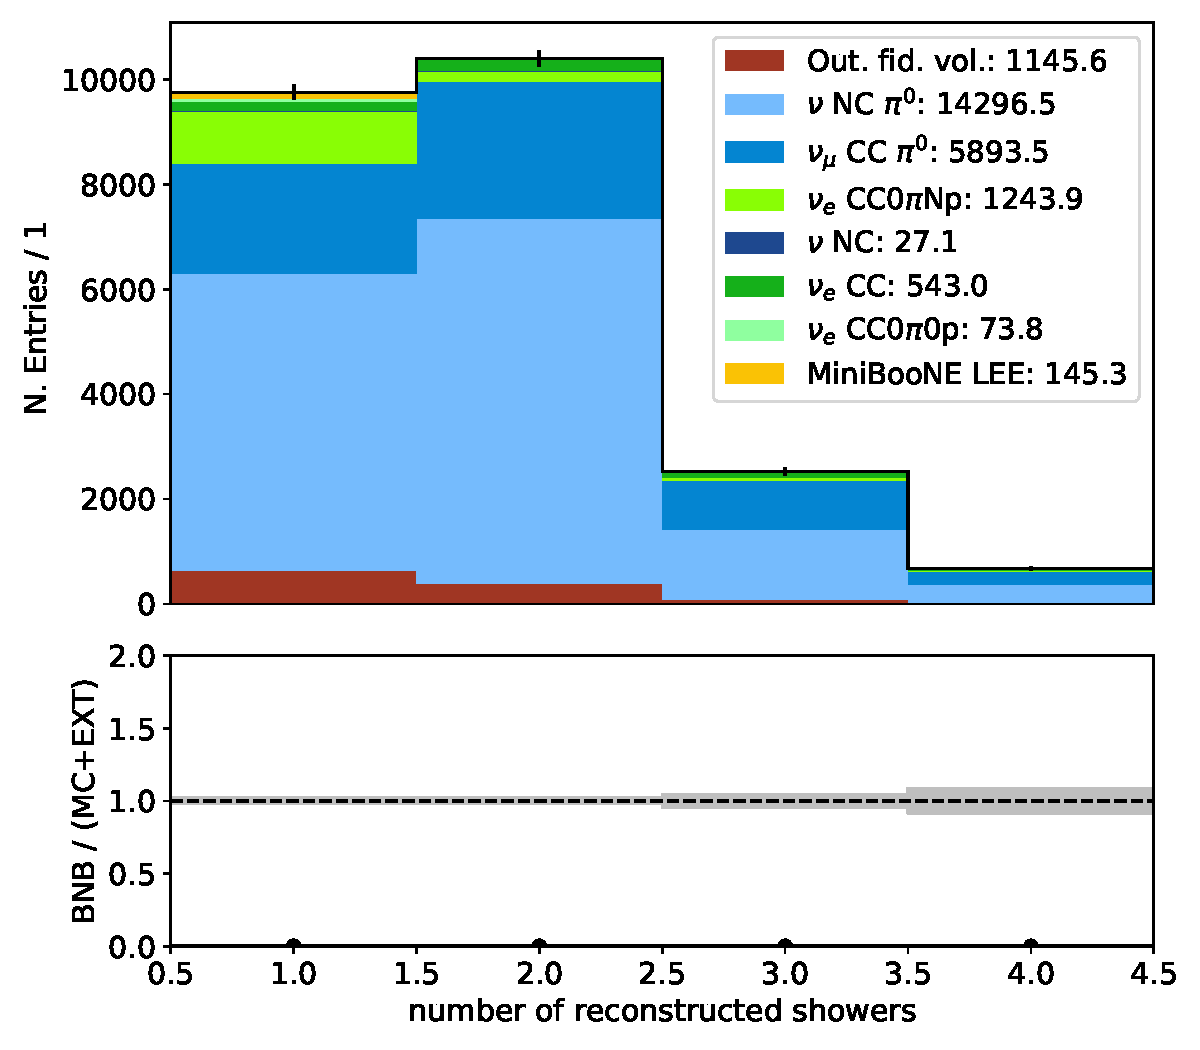
\includegraphics[width=1.00\textwidth]{egamma/n_showers_contained_01022020.pdf}
    \caption{number of reconstructed showers}
    \end{subfigure}
    \begin{subfigure}[b]{0.31\textwidth}
    \centering
    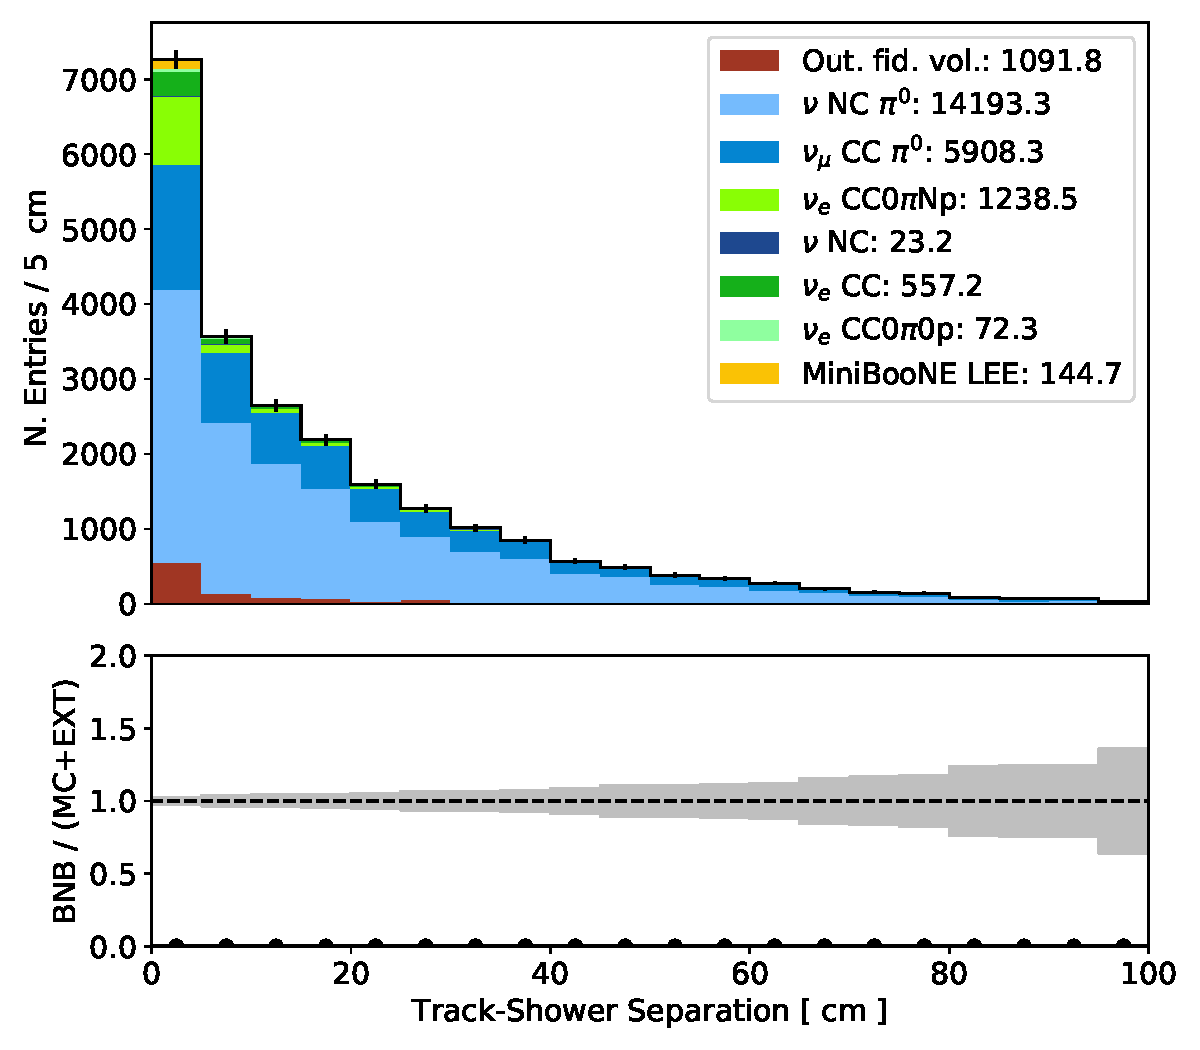
\includegraphics[width=1.00\textwidth]{egamma/tksh_distance_01022020.pdf}
    \caption{track-shower separation}
    \end{subfigure}
    \begin{subfigure}[b]{0.31\textwidth}
    \centering
    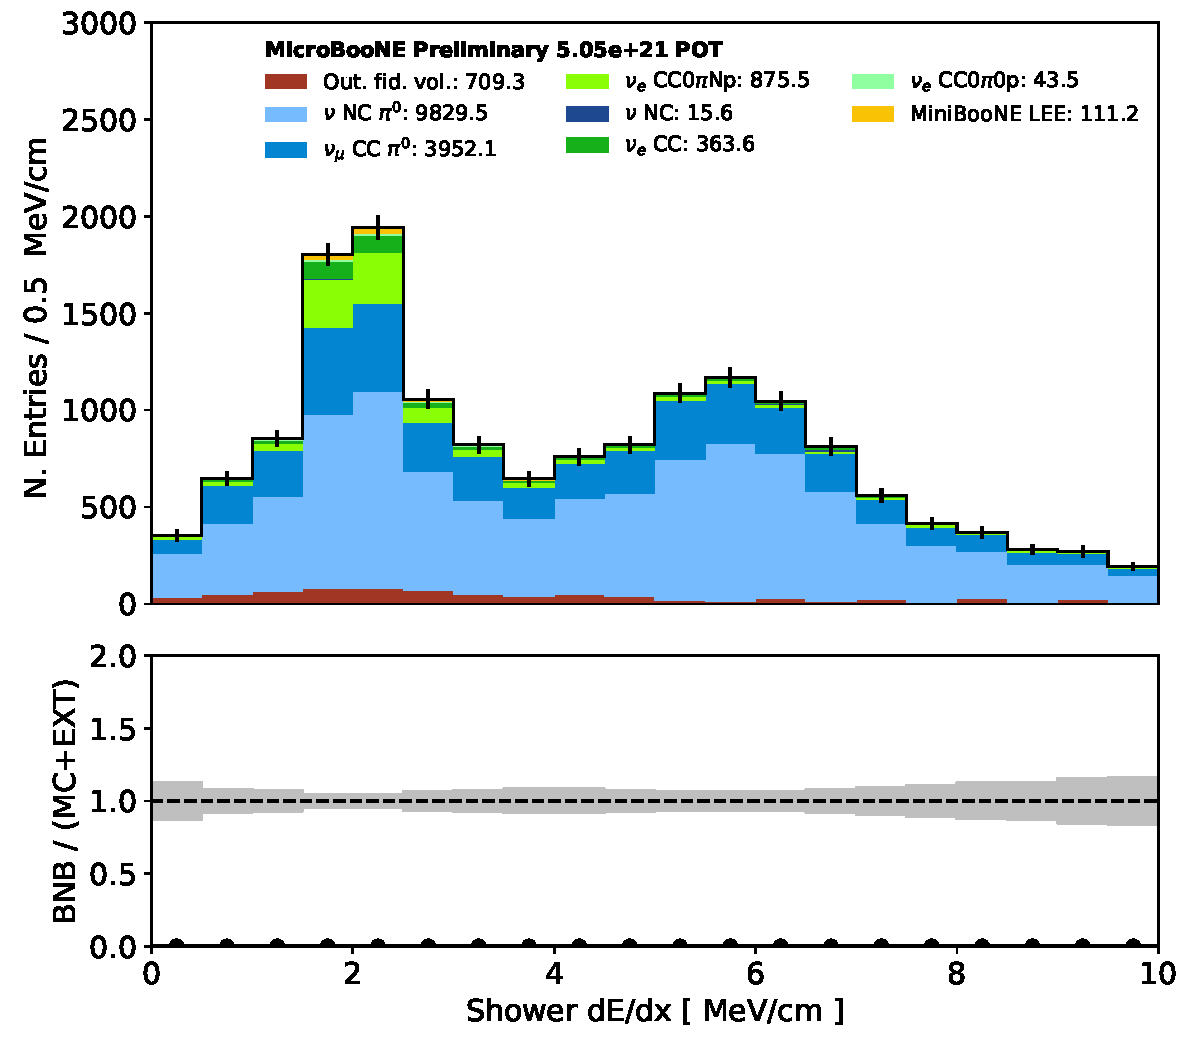
\includegraphics[width=1.00\textwidth]{egamma/shr_tkfit_dedx_Y_01022020.pdf}
    \caption{\label{fig:egammasep:dedx} reconstructed shower $dE$/$dx$}
    \end{subfigure}
\caption{\label{fig:egammasep}Comparison of simulated $\nu_e$ (green) vs. $\nu_{\mu} \rightarrow \pi^0 + X$ (blue) for the three discriminating variables of (a) number of showers, (b) vertex distance, and (c) $dE$/$dx$. Distributions are POT-normalized but do not conatain non-$\nu_e$ or non-$\pi^0$ events, nor on/off-beam data distributions.}
\end{center}
\end{figure}

\par \textbf{two-shower requirement} Requiring a single reconstructed shower retains 68\% of $\nu_e$ interactions (with no $\pi^0$ in the final state) while removing 61\% of $\nu_{\mu}$ events with at least one $\pi^0$ in the final state. The fraction of selected $\nu_e$s grows to 79\% when looking below 800 MeV of true energy (the focus of this analysis). Rejection of $\nu_e$s is largely due to events where the electron shower is reconstructed as two separate EM showers, often closely aligned in 3D. Events with final state $\pi^0$s are reconstructed with a single EM shower in the final state because either the second photon escapes the TPC active volume completely (irreducible) or because the second shower is not reconstructed. The dominant causes of this second case are (1) highly-boosted $\pi^0$ decays, in which two aligned photons are merged into one shower and (2) photons which go undetected, often low in energy (below 100 MeV). Additional discriminating variables which aim to recover the reconstruction-related mis-ID of (1) and (2) are utilized in the analysis and presented in Sec.~\ref{sec:nueselection:inputs}.
\par \textbf{track-shower separation} For events where hadronic activity at the neutrino interaction vertex (i.e. final-state protons) is visible, a clear gap between the vertex and the shower start-point can be used to reject $\gamma$ backgrounds. This is a powerful background mitigation tool in the 1$e$N$p$ $\nu_e$ selection. Two factors determine the performance of such a tool: the ability to detect protons and other hadronic activity at the vertex and the accuracy with which the shower start-point is reconstructed. The shower start-point reconstruction accuracy determines the level of background rejection one can obtain, as $\gamma$ showers lead to an exponential conversion-distance distribution. A 1 vs. 5 cm track-shower separation cuts lead to 95\% vs 74\% mis-ID respectively, but causes a drop in selection efficiency for 1$e$N$p$ events from 72\% to 28\%. This is a consequence of the sub-optimal vertex reconstruction accuracy for low-energy $\nu_e$ interactions. In order to enhance the ability to isolate $\nu_e$ events in the 1$e$N$p$ selection through vertex-displacement, different metrics are used to measure the presence of a gap between an electron and proton candidate. These will be described in section~\ref{sec:nueselection:inputs}. It is important to note that this background mitigation strategy is not applicable to single-electron searches, which are an important contribution to $\nu_e$ interactions, especially in the low-energy regime.
\par \textbf{shower d$E$/d$x$} The majority of photons manifest themselves in the TPC through the ionization released by the $e^+$/$e^-$ pair produced via pair-conversion. The electron-positron pair is highly aligned and overlaps on the mm-scale, leading to a doubly-ionizing charge-segment compared to electron showers. To measure this, we use the track fit of the main shower trunk and the calorimetric tools as described in Sec.~\ref{sec:tkshreco}. 
%with a modified version of the MicroBooNE track-fitter~\cite{bib:shrtrackfitter} and for each point along a track the d$Q$/d$x$  and distance from the shower-start are recorded using MicroBooNE's Calorimetry module. This procedure allows to accurately measure d$x$, including small deflections due to the electron's trajectory and SCE offsets, and d$Q$, by incorporating MicroBooNE's full position- and field-dependent relative and absolute charge calibration. From d$Q$/d$x$, d$E$/d$x$ is calculated assuming a fixed recombination correction assuming 2.1 MeV/cm energy loss, but accounting for local variations in the electric field. 
The distinctive 4 MeV/cm population expected for $\gamma$ showers is visible in figure~\ref{fig:egammasep:dedx}. The main limitation to $e$/$\gamma$ separation via d$E$/d$x$ is the large fraction of photons reconstructed with a d$E$/d$x$ of less then 3 MeV/cm (23\% of $\pi^0$ events fall in the 1-3 MeV range). This is due both to mis-reconstructed events, for which the start-point is incorrectly reconstructed by more than one or two cm, and to events where the photon shower's energy loss-profile is not as clearly distinguishable from that of a single electron. While the relative contribution of these two sources is still under determination, the second causes a significant mis-ID rate, and is largely associated to lower-energy $\gamma$ showers for which the production of a highly asymmetric electron-positron pair where one of the electrons is barely visible is more frequent. The impact of shower energy on the measured d$E$/d$x$ for a $\gamma$ shower is shown in figure~\ref{fig:dedxgammas:energy}. Below 100 MeV, where most $\gamma$ showers in the BNB are produced, the reconstructed d$E$/d$x$ is electron-like. The impact of distance from the shower start-point on whether d$E$/d$x$ is reconstructed to be 2 or 4 MeV/cm is also important, as can be seen in figure~\ref{fig:dedxgammas:dist}. This is particularly true for low-energy asymmetric pair-production events, and motivates utilizing 
d$E$/d$x$ information at different distances from the shower start-point for $e$/$\gamma$ separation.
\begin{figure}[H] 
\begin{center}
    \begin{subfigure}[b]{0.45\textwidth}
    \centering
    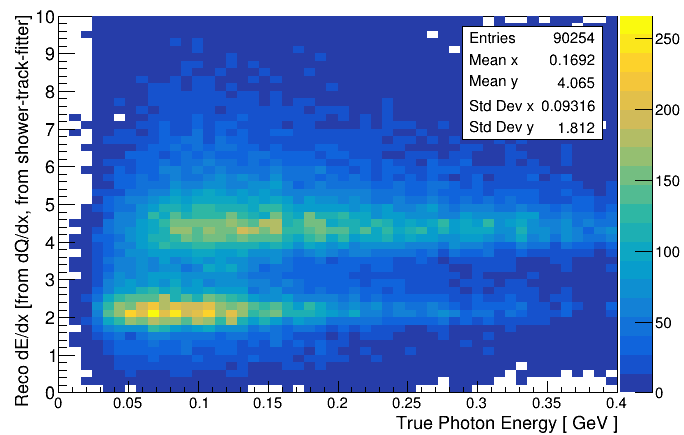
\includegraphics[width=1.00\textwidth]{egamma/dedx_vs_energy_gamma.png}
    \caption{\label{fig:dedxgammas:energy} d$E$/d$x$ vs. distance from shower start-point for $\gamma$ showers}
    \end{subfigure}
    \begin{subfigure}[b]{0.45\textwidth}
    \centering
    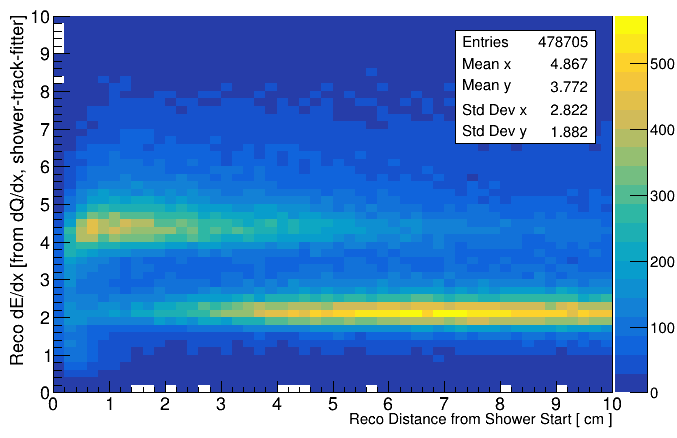
\includegraphics[width=1.00\textwidth]{egamma/dedx_vs_dist_gamma.png}
    \caption{\label{fig:dedxgammas:dist} d$E$/d$x$ vs. distance from shower start-point for $\gamma$ showers}
    \end{subfigure}
\caption{\label{fig:dedxgammas}}
\end{center}
\end{figure}



\newpage

\subsection{Energy Reconstruction \textcolor{green}{Giuseppe + David}}
\label{sec:ereco}
\par Energy reconstruction is performed calorimetrically for EM showers and through a measurement of a track's range for contained muons and protons. For muons multiple Coulomb scattering (MCS) is also used to estimate the muon energy. The energy resolution obtained for different particles is reported in table~\ref{tab:eres}. More information on each particle specie's energy resolution is reported in figure~\ref{fig:eres:particle} where for each particle species the 2D reconstructed vs. true energy distribution (in log-scale) is shown on the left, next to a plot of energy resolution vs. true energy on the right. The energy resolution reported here is obtained from a Gaussian plus one-sided exponential fit to the distribution $[E_{\rm reco}-E_{\rm true}] / E_{\rm true}$. The resolution reported refers only to the Gaussian width $\sigma$ extracted in the fit, and therefore does not account for negative tails, which are significant in the case of EM shower energy reconstruction, and described below.


\begin{table}[H]
\centering
  \begin{tabular}{ | c | c |  }
    \hline
    particle & kinetic energy resolution  \\ \hline
    proton & 4\% at 100 MeV 1\% at 200 MeV \\ \hline
    muon (range) & 3\%  \\ \hline
    muon (MCS) & $\frac{4.7\%}{\sqrt{E/{\rm GeV}}} \otimes \frac{2.8\%}{E/{\rm GeV}} \otimes 0.0\%$  \\ \hline
    electron & 15\%  \\
    \hline
    
  \end{tabular}
  \caption{\label{tab:eres} Energy resolution for different particle species.}
 \end{table}
 
 \par For EM showers, the calorimetric energy reconstruction response has a significant non-Gaussian component, as well as a large bias. Both effects are attributable to reconstruction effects associated with under-clustering of charge. The energy bias is found to be 20\% and approximately flat in energy, and motivates a definition of a corrected shower energy, defined as $E_{\rm corrected} = E_{\rm calorimetry} / 0.8$. The non-Gaussian response for EM energy reconstruction can be modeled through a Gaussian plus one-sided exponential distribution. Figure~\ref{fig:eres:elec:binned} shows in different bins of true energy the fractional energy response and a fit to a Gaussian plus one-sided exponential function. The residual energy bias, after the 20\% correction applied, is of order $3-8$\%. 
 
 \begin{figure}[ht]
\begin{center}
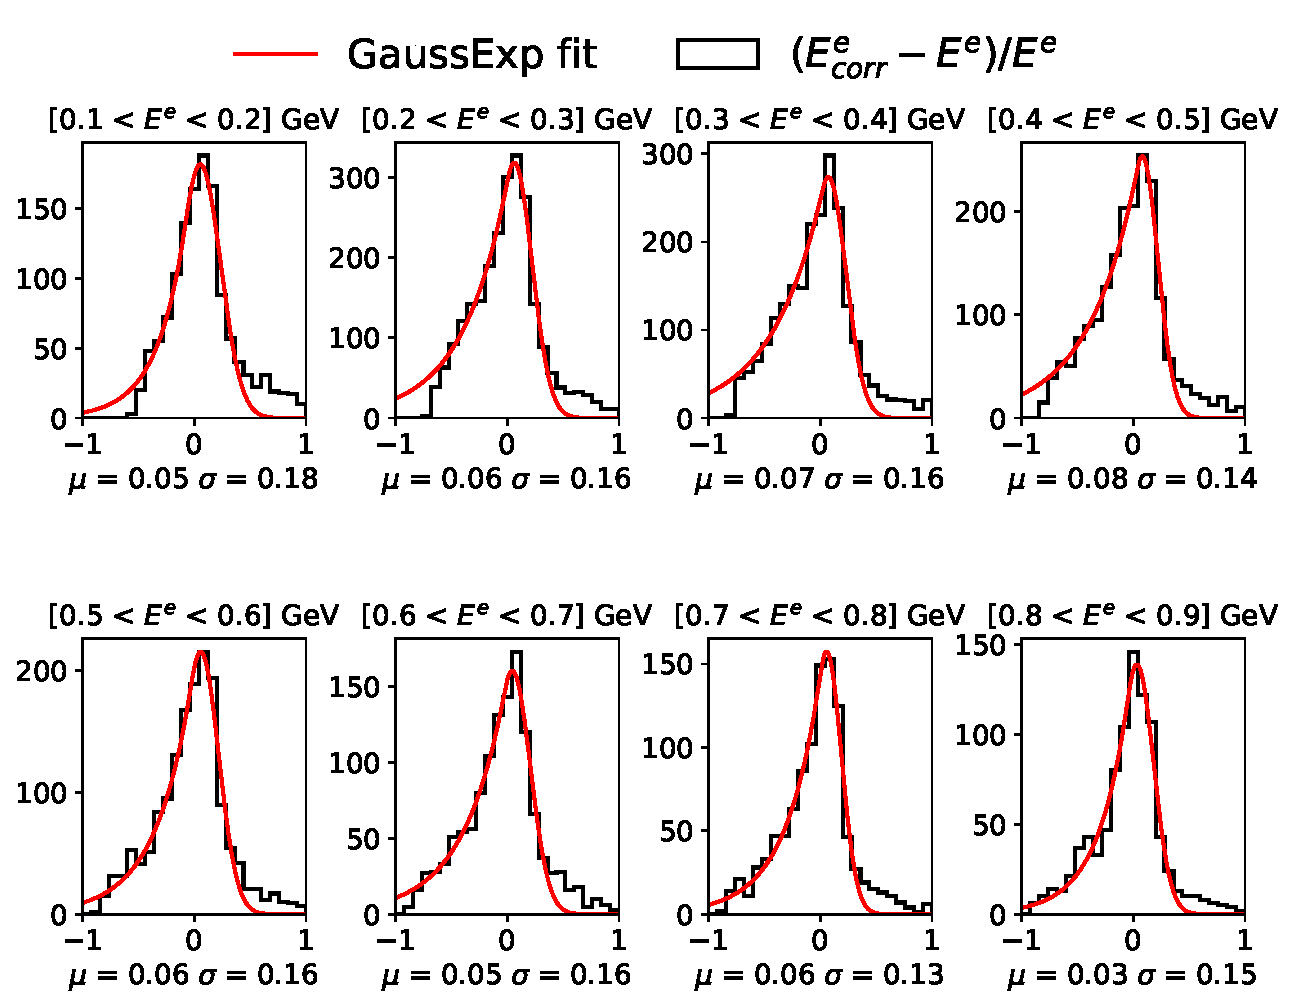
\includegraphics[width=0.75\textwidth]{ereco/elec_eres_binned.pdf}
\caption{\label{fig:eres:elec:binned}Energy resolution for electron showers.}
\end{center}
\end{figure}
 
 \newpage

\begin{figure}[H] 
\begin{center}
    \begin{subfigure}[b]{0.4\textwidth}
    \centering
    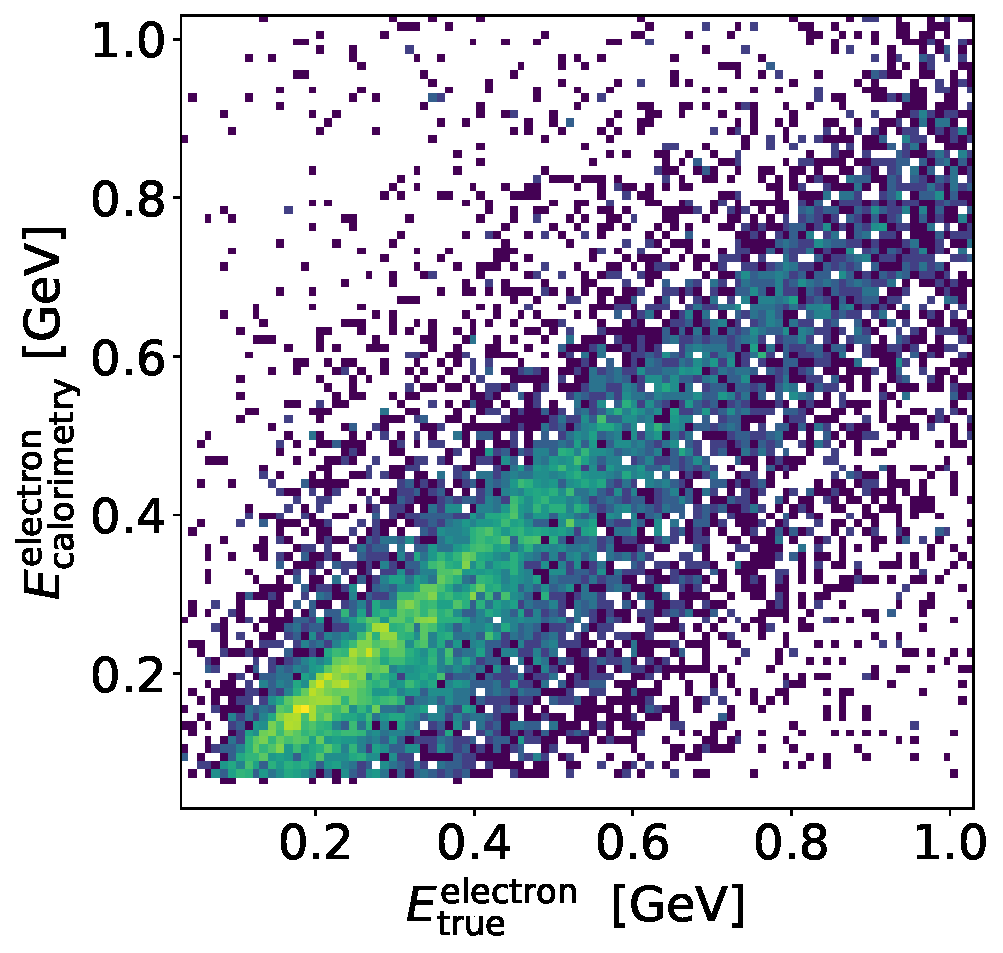
\includegraphics[width=1.00\textwidth]{ereco/electron_eres2D.pdf}
    %\caption{\label{fig:eres:elec:2d} }
    \end{subfigure}
    \begin{subfigure}[b]{0.38\textwidth}
    \centering
    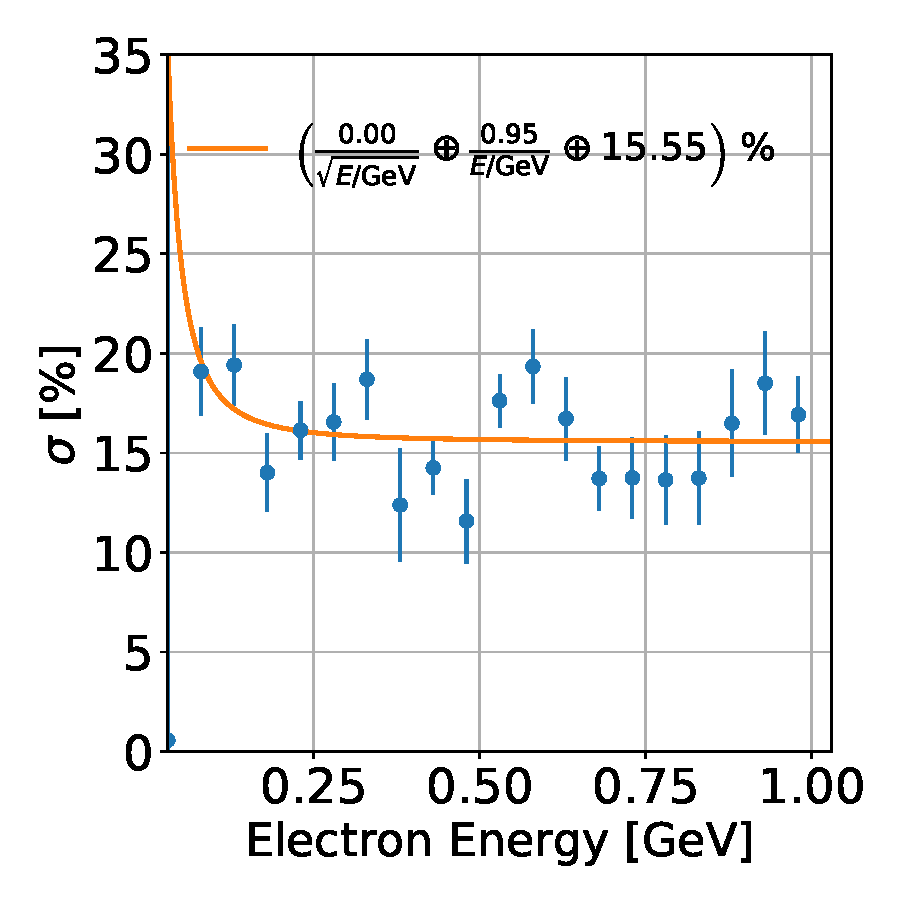
\includegraphics[width=1.00\textwidth]{ereco/elec_eres_vs_true.pdf}
    %\caption{\label{fig:eres:elec:vstrue} }
    \end{subfigure}
    \begin{subfigure}[b]{0.4\textwidth}
    \centering
    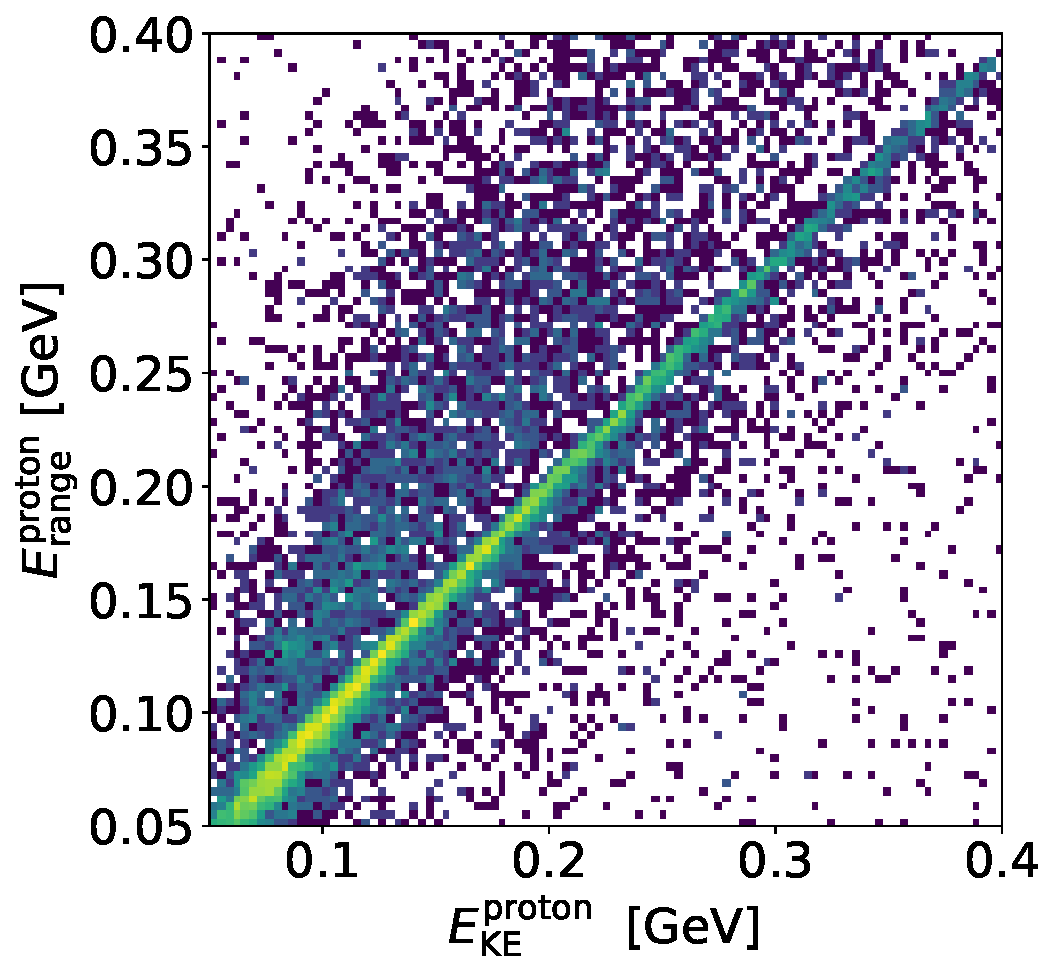
\includegraphics[width=1.00\textwidth]{ereco/proton_eres2D.pdf}
    %\caption{\label{fig:eres:proton:2d} }
    \end{subfigure}
    \begin{subfigure}[b]{0.38\textwidth}
    \centering
    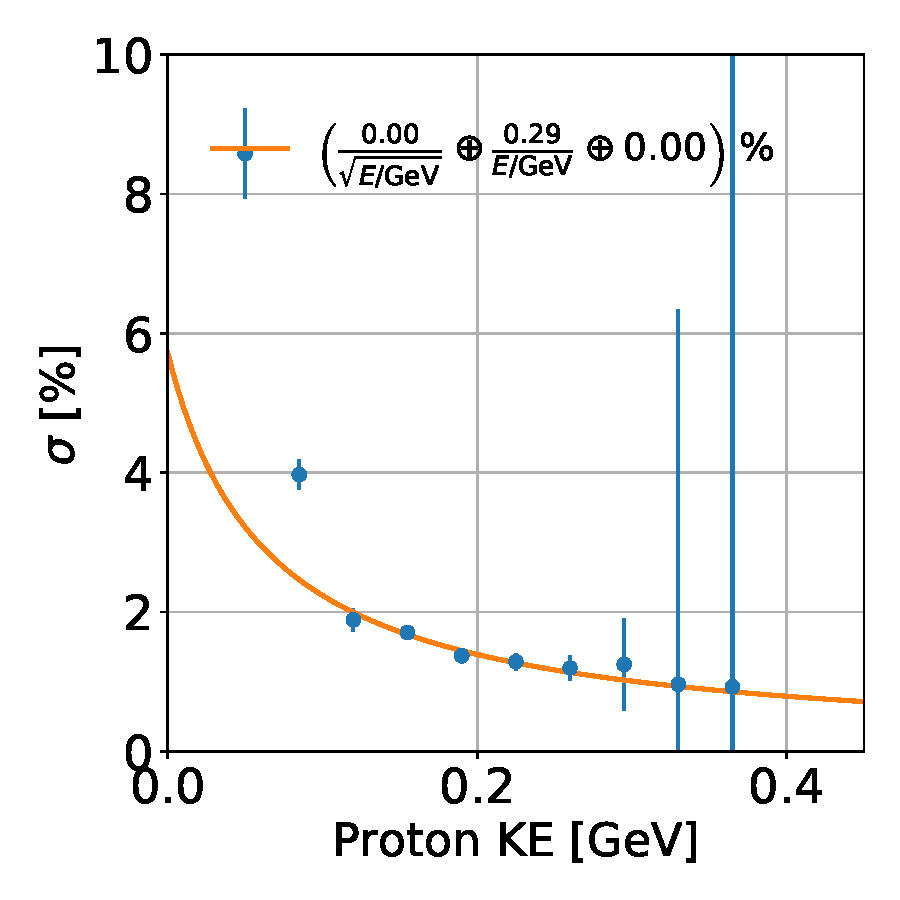
\includegraphics[width=1.00\textwidth]{ereco/proton_eres_vs_true.pdf}
    %\caption{\label{fig:eres:proton:vstrue} }
    \end{subfigure}
    \begin{subfigure}[b]{0.4\textwidth}
    \centering
    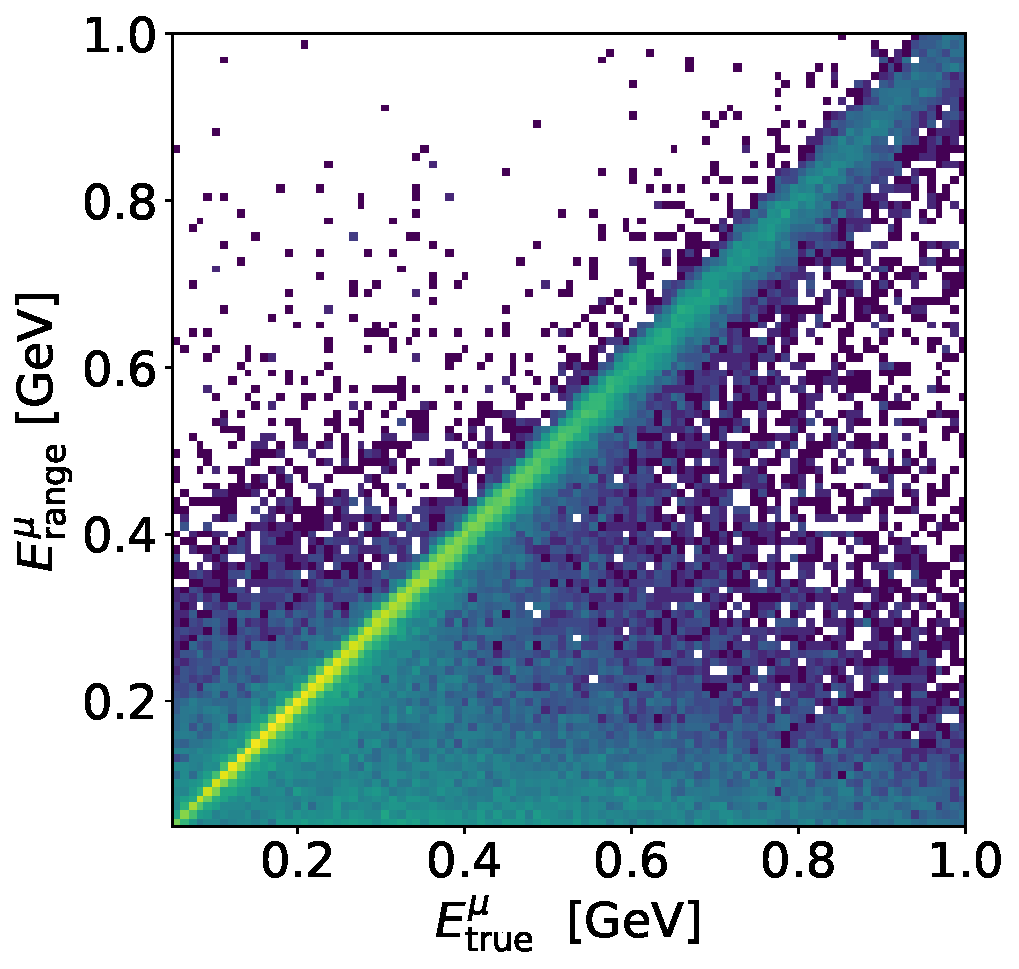
\includegraphics[width=1.00\textwidth]{ereco/muon_range_eres2D.pdf}
    %\caption{\label{fig:eres:muon:2d} }
    \end{subfigure}
    \begin{subfigure}[b]{0.38\textwidth}
    \centering
    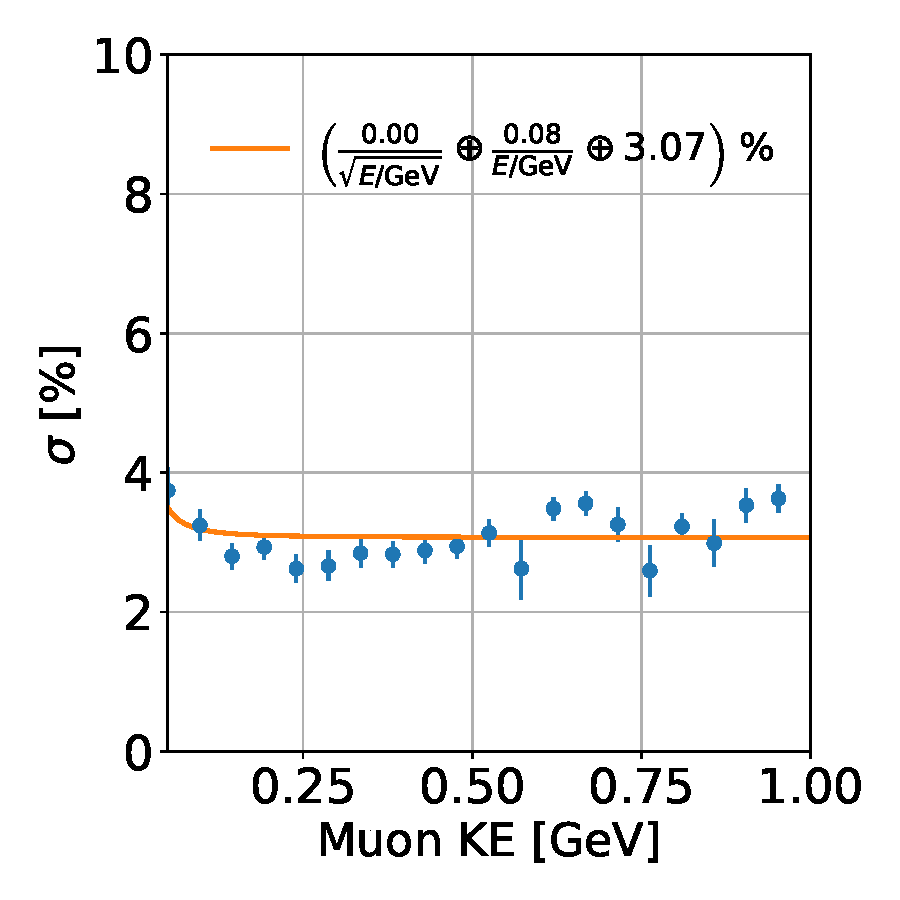
\includegraphics[width=1.00\textwidth]{ereco/muon_range_eres_vs_true.pdf}
    %\caption{\label{fig:eres:muon:vstrue} }
    \end{subfigure}
\caption{\label{fig:eres:particle}Energy resolution for electrons (top), protons (center) and muons (bottom). Left: reconstructed vs. true energy resolution (log-scale). Right: energy resolution from Gaussian fit to $[E_{\rm reco}-E_{\rm true}] / E_{\rm true}$.}
\end{center}
\end{figure}

\newpage

\subsubsection{Neutrino Energy Reconstruction \textcolor{green}{Giuseppe + David}}

\par In this analysis, the energy reconstruction for neutrino interactions is performed through a sum of the visible energy of the various reconstructed final-state particles in the interaction. For $\nu_e$ events the reconstructed energy is defined as:
\begin{equation}
    E_{\rm reco}^{\nu_e} = E_{\rm corrected}^{\rm electron} + \sum_{\rm tracks} E_{\rm range}^{\rm proton}
\end{equation}{}

For contained $\nu_{\mu}$ interactions, the reconstructed energy is defined as:

\begin{equation}
    E_{\rm reco}^{\nu_{\mu}} = E_{\rm range}^{\rm muon} + \sum_{\rm protons} E_{\rm range}^{\rm proton} + 0.105 \; GeV
\end{equation}{}

Figure~\ref{fig:eres:neutrino} shows the comparison between reconstructed energy and truth visible energy, which is defined as the sum of the lepton energy, pion energy (if present), and proton energy (for all protons above 40 MeV of KE). This comparison shows very accurate energy reconstruction for $\nu_{\mu}$ events. For $\nu_e$ interactions, with smearing dominated by the worse energy resolution of electron showers.

\begin{figure}[H] 
\begin{center}
    \begin{subfigure}[b]{0.4\textwidth}
    \centering
    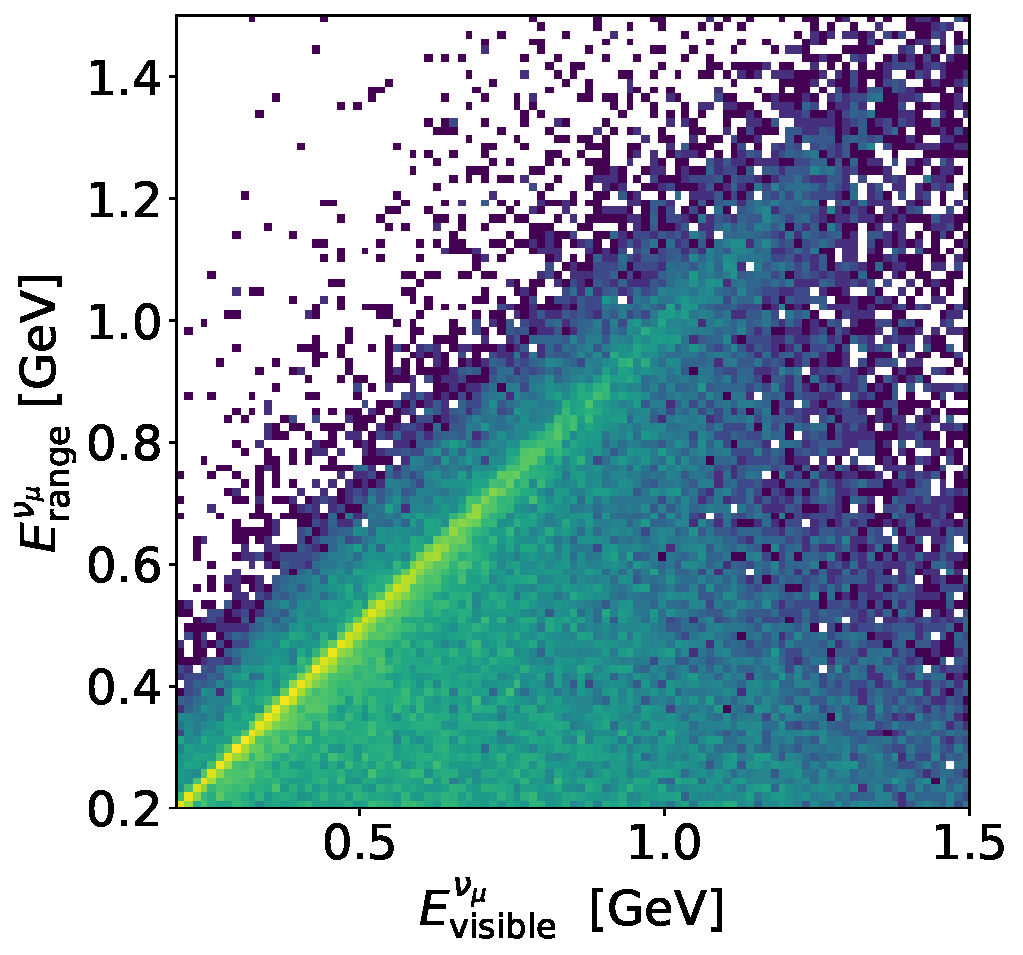
\includegraphics[width=1.00\textwidth]{ereco/numu_energy_visible_eres2D.pdf}
    \caption{\label{fig:eres:numu:2d} }
    \end{subfigure}
    \begin{subfigure}[b]{0.4\textwidth}
    \centering
    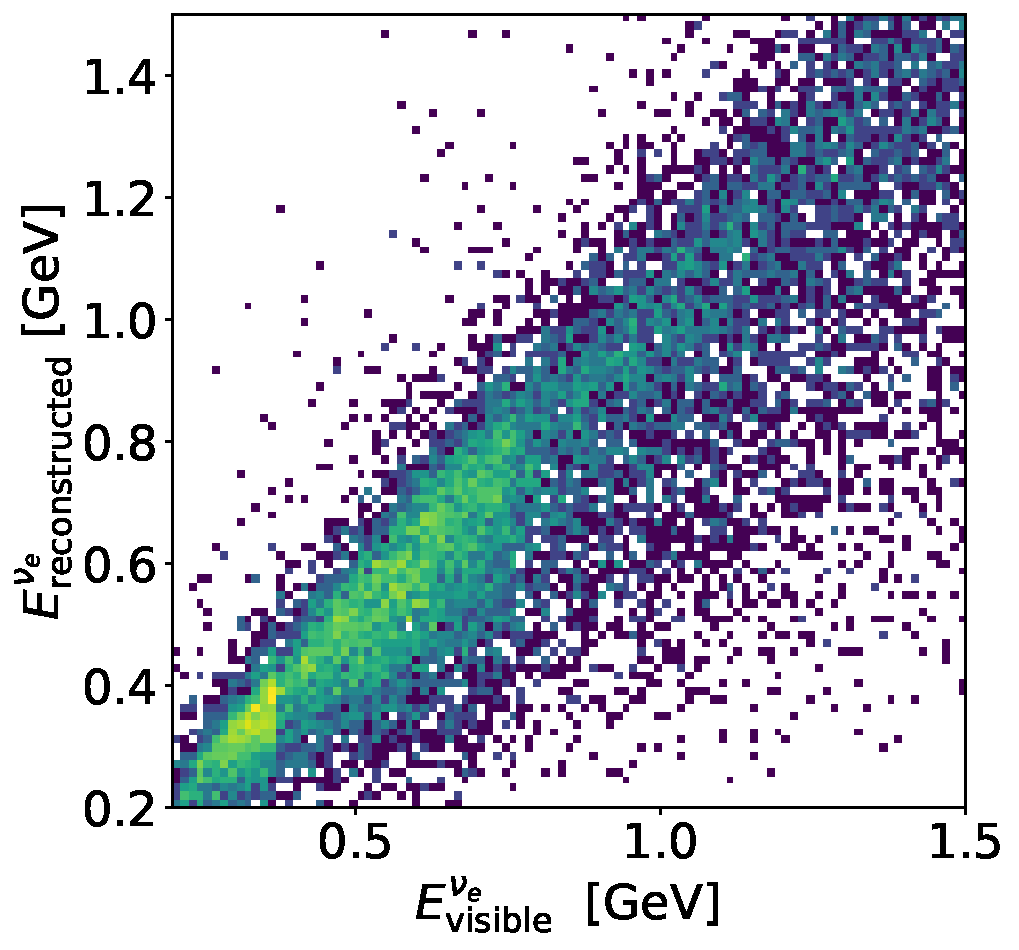
\includegraphics[width=1.00\textwidth]{ereco/nue_visible_eres2D.pdf}
    \caption{\label{fig:eres:nue:vstrue} }
    \end{subfigure}
\caption{\label{fig:eres:neutrino}Log-scale color-maps.}
\end{center}
\end{figure}

\newpage

\section{Control Samples and Analysis Input Validation}
\par The selections and analysis described below rely on well understood detector, simulation, calibration, and analysis tools performance. This section is dedicated to evaluating the performance of detector modeling through data-mc comparisons of targeted sidebands. The sidebands developed for this analysis are a high-stats $\pi^0$ selection, and an \emph{anti-BDT} filter which targets the selection of $\nu_e$ like backgrounds. Currently comparisons for the \emph{anti-BDT} filter are not available and will be documented in a future iteration of this note.
\par It is important to note that in addition to detector simulation and reconstruction effects, $\nu$-Ar modeling can impact the level of data-mc agreement in various variables. We will try to point out when this might be the case.
\subsection{$\pi^0$ control sample \textcolor{green}{David}}
\par A $\pi^0$ selection has been developed in order to obtain high-stats samples of $\pi^0$ events and $\gamma$ EM showers which can constrain $\pi^0$ production modeling uncertainties as well as validate the analyis' ability to reconstruct and select EM showers.
\par Figure~\ref{fig:pi0:mass} shows the reconstructed $M\gamma\gamma$ for candidate $\pi^0$ events, with a calibrated but uncorrected (i.e. not accounting for biases in shower energy reconstruction caused by the incompleteness in charge clustering) energy reconstruction. Overall there is good data-MC agreement, apart from an apparent normalization difference. To account for this normalization difference we measure a flat scaling factor needed for CC and NC $\pi^0$ events needed to obtain  consitent rate in data and MC. This factor is found to be 72.4\% in Run1 and 72.7\% in Run3. We repeat the exercise applying a tighter $\pi^0$ selection enhancing the $\pi^0$ purity and obtain scaling factors of 70\% for both Run1 and Run3. While this procedure is far from rigorous, it allows us to study detector-related and specifically shower-related variables removing a large normalization difference. \textcolor{red}{A more rigorous data-driven constrain of our $\pi^0$ rate, performed accounting for detector and flux systematics, and considering a broader range of $\pi^0$ modeling, will need to be performed.}

\begin{figure}[H] 
\begin{center}
    \begin{subfigure}[b]{0.3\textwidth}
    \centering
    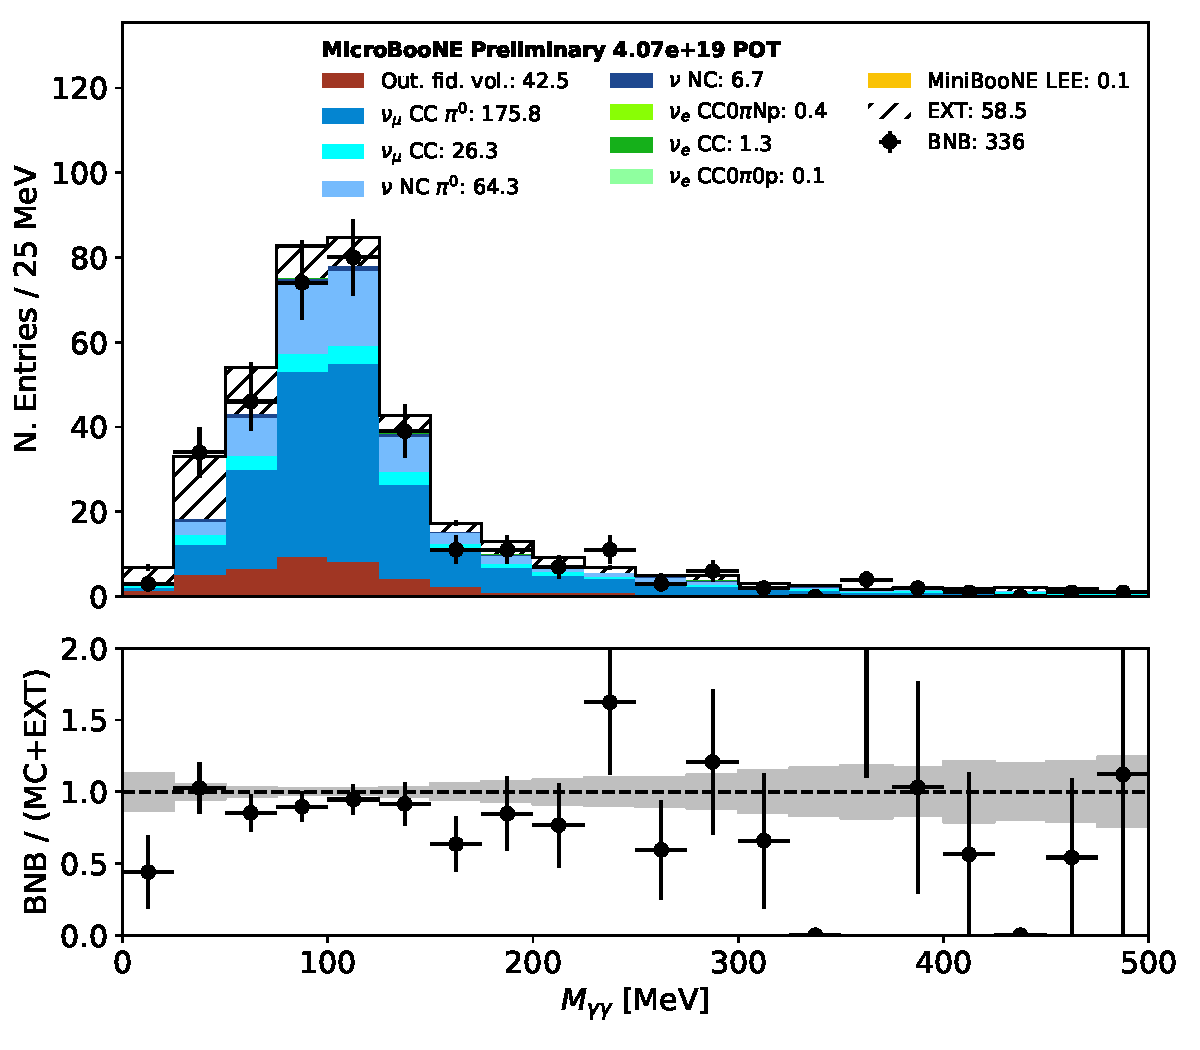
\includegraphics[width=1.00\textwidth]{pi0/pi0_mass_Y_01142020_5E19.pdf}
    \caption{\label{fig:pi0:mass:5E19} Run 1 ``5E19'' open dataset.}
    \end{subfigure}
    \begin{subfigure}[b]{0.3\textwidth}
    \centering
    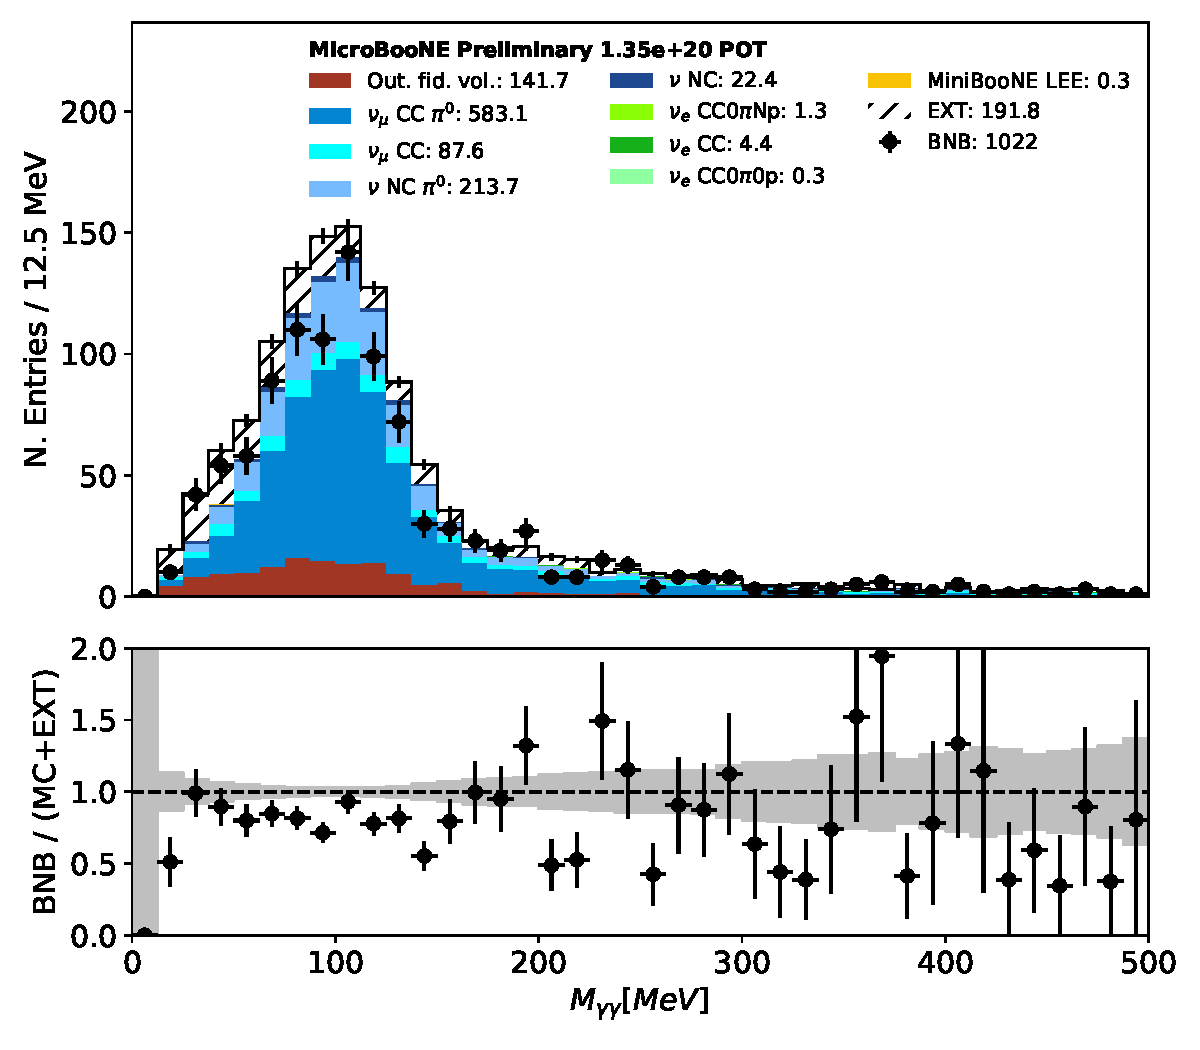
\includegraphics[width=1.00\textwidth]{pi0/pi0_mass_Y_01142020sel__RUN1.pdf}
    \caption{\label{fig:pi0:mass:5E19} Run 1.}
    \end{subfigure}
    \begin{subfigure}[b]{0.3\textwidth}
    \centering
    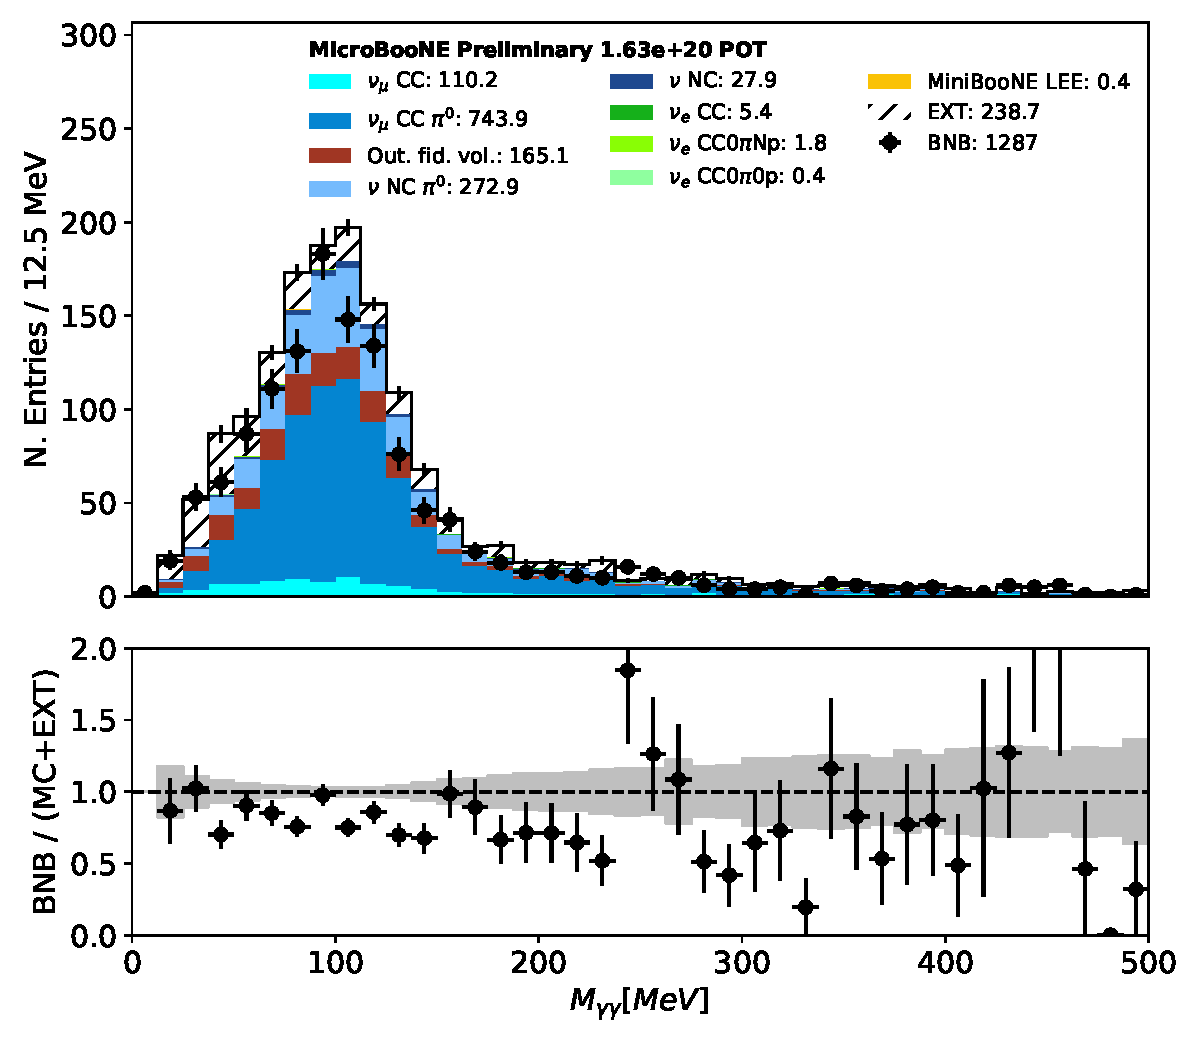
\includegraphics[width=1.00\textwidth]{pi0/pi0_mass_Y_01142020sel_RUN3.pdf}
    \caption{\label{fig:pi0:mass:5E19} Run 3.}
    \end{subfigure}
\caption{\label{fig:pi0:mass}Reconstructed $\pi^0$ mass.}
\end{center}
\end{figure}

\par After applying a scaling factor of 0.7 to CC and NC $\pi^0$ events in the MC, we show comparisons of shower variables with the goal of assessing data-mc agreement for the $\nu_e$ selection. Figure~\ref{fig:pi0:datamc} shows reconstructed quantities used in the $\nu_e$ analysis for $\pi^0$ candidate events which are useful in validating the rubstness of shower modeling. They include leading and sub-leading shower dE/dx (top), followed by the leading and sub-leading shower conversion distance and shower score. The last row reports the reconstructed shower Moliere angle and track PID score for the longest track in each event. Generally, the data-MC agreement is quite good. For d$E$/d$x$ there appears to be a clear distortion, specifically in the 4 MeV/cm peak associated with photons. \textcolor{red}{A re-calibration of shower d$E$/d$x$ is planned for the analysis, but has not been fully implemented as of now.}

\begin{figure}[H] 
\begin{center}
    \begin{subfigure}[b]{0.38\textwidth}
    \centering
    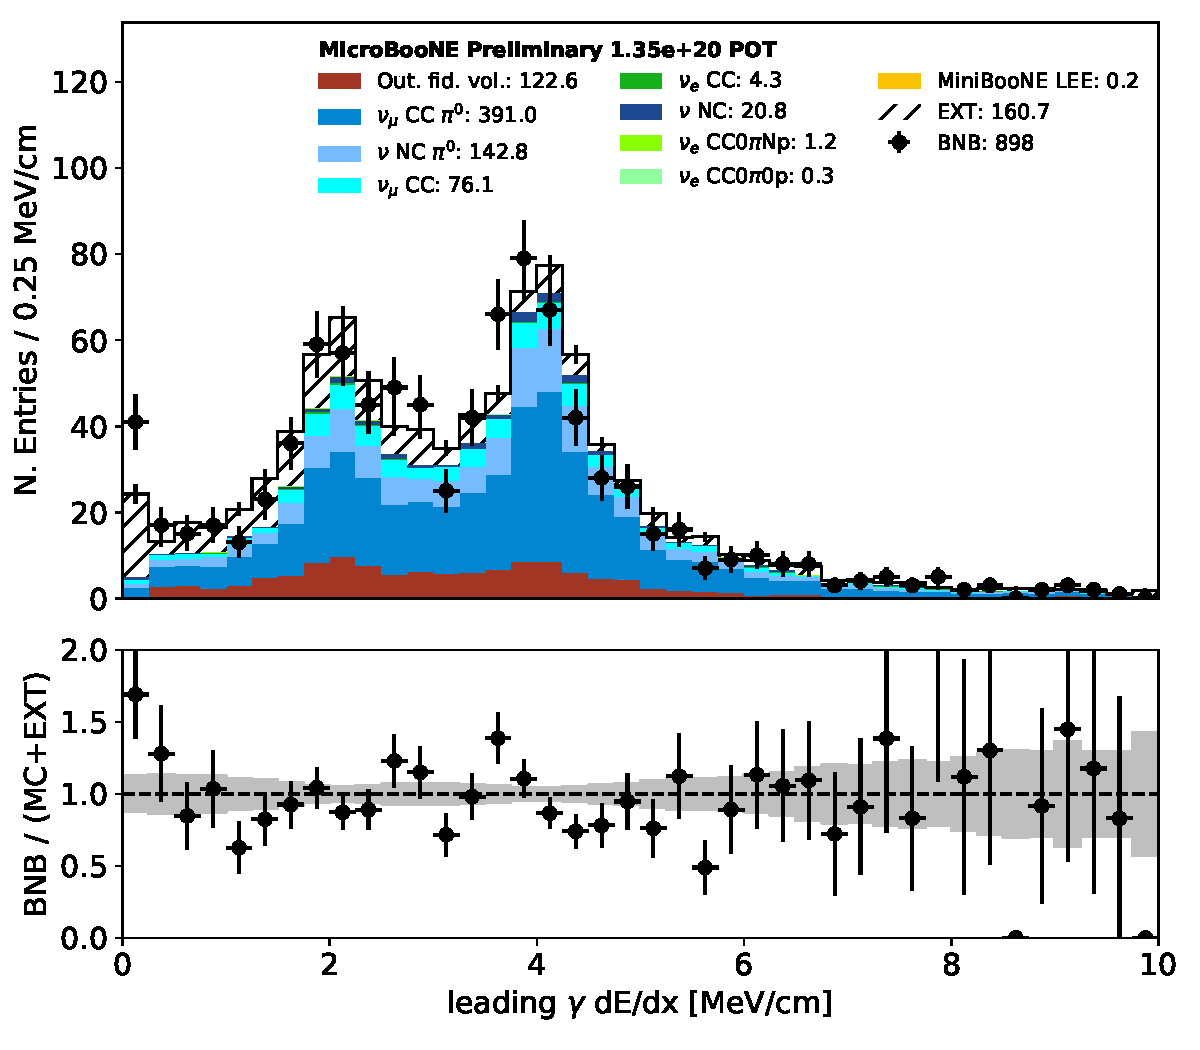
\includegraphics[width=1.00\textwidth]{pi0/pi0_dedx1_fit_Y_01152020_scaled_RUN1.pdf}
    %\caption{\label{fig:pi0:dedx:RUN1:leading} Run 1 leading shower.}
    \end{subfigure}
    \begin{subfigure}[b]{0.38\textwidth}
    \centering
    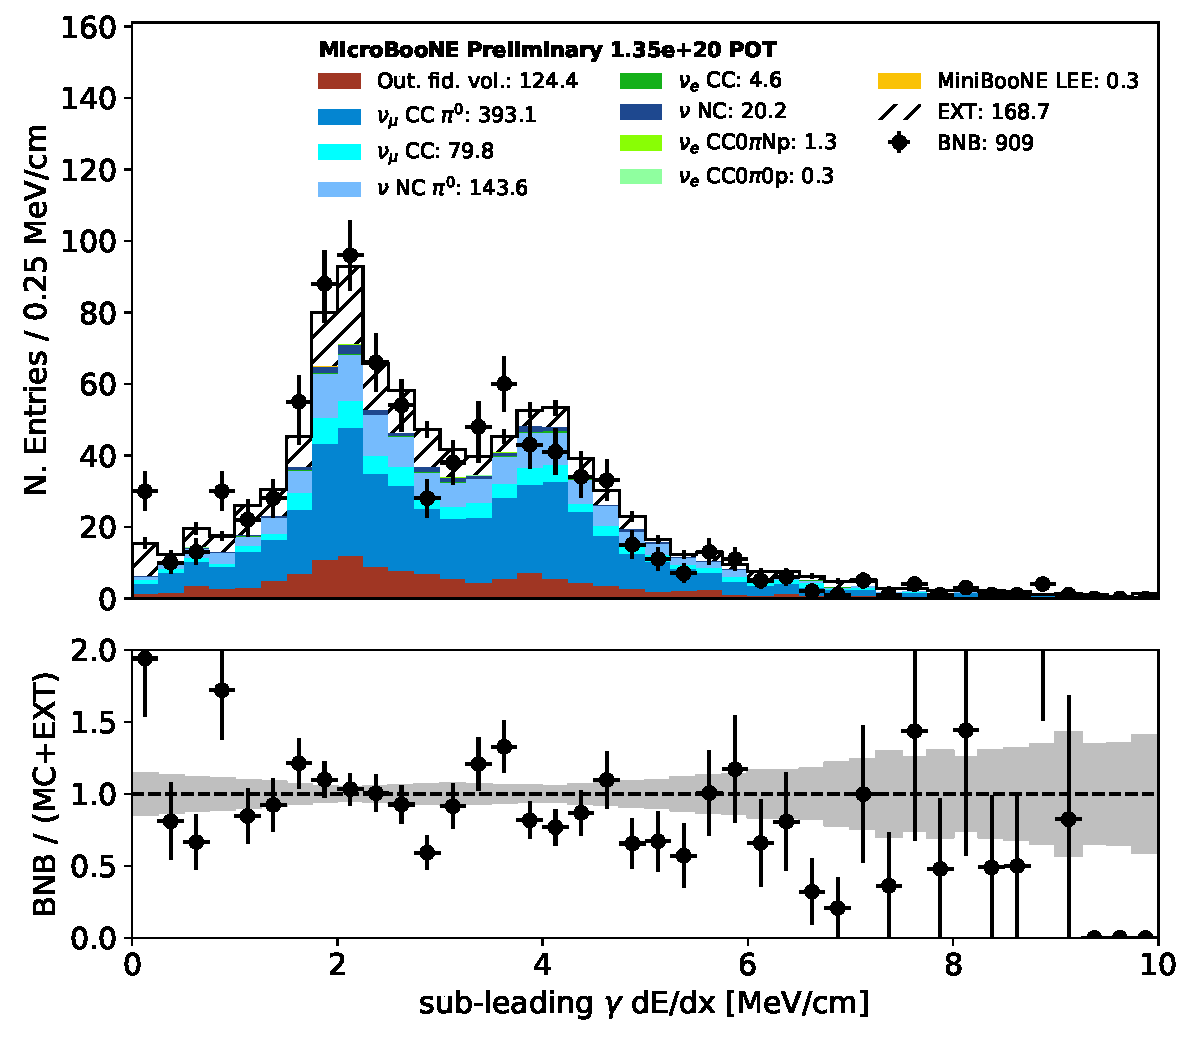
\includegraphics[width=1.00\textwidth]{pi0/pi0_dedx2_fit_Y_01152020_scaled_RUN1.pdf}
    %\caption{\label{fig:pi0:dedx:RUN1:subleading} Run 1 sub-leading shower.}
    \end{subfigure}
    
    \begin{subfigure}[b]{0.38\textwidth}
    \centering
    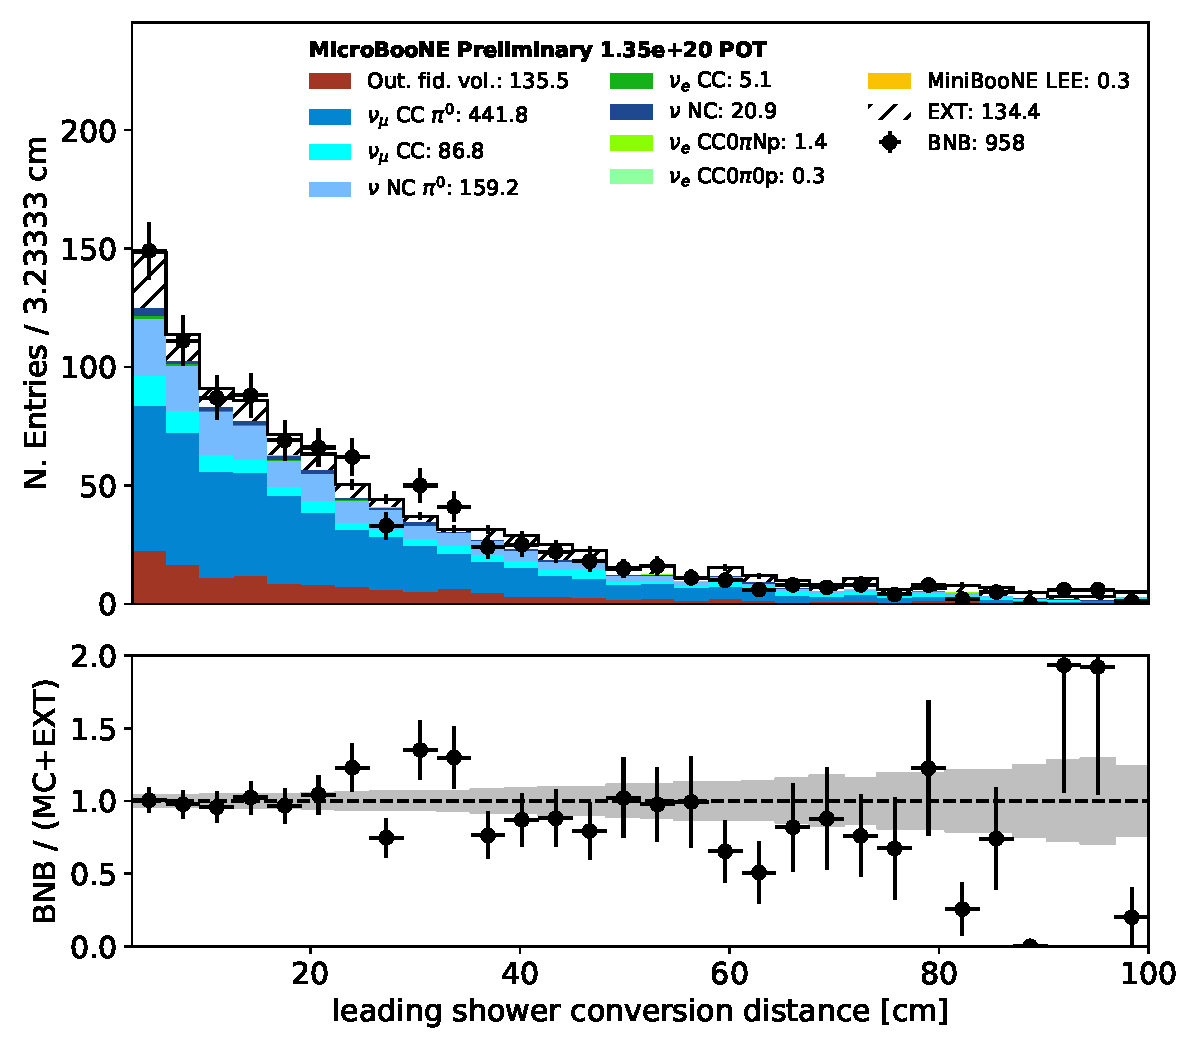
\includegraphics[width=1.00\textwidth]{pi0/pi0_radlen1_01152020_inputs_RUN1.pdf}
    %\caption{\label{fig:pi0:dedx:RUN1:leading} Run 1 leading shower.}
    \end{subfigure}
    \begin{subfigure}[b]{0.38\textwidth}
    \centering
    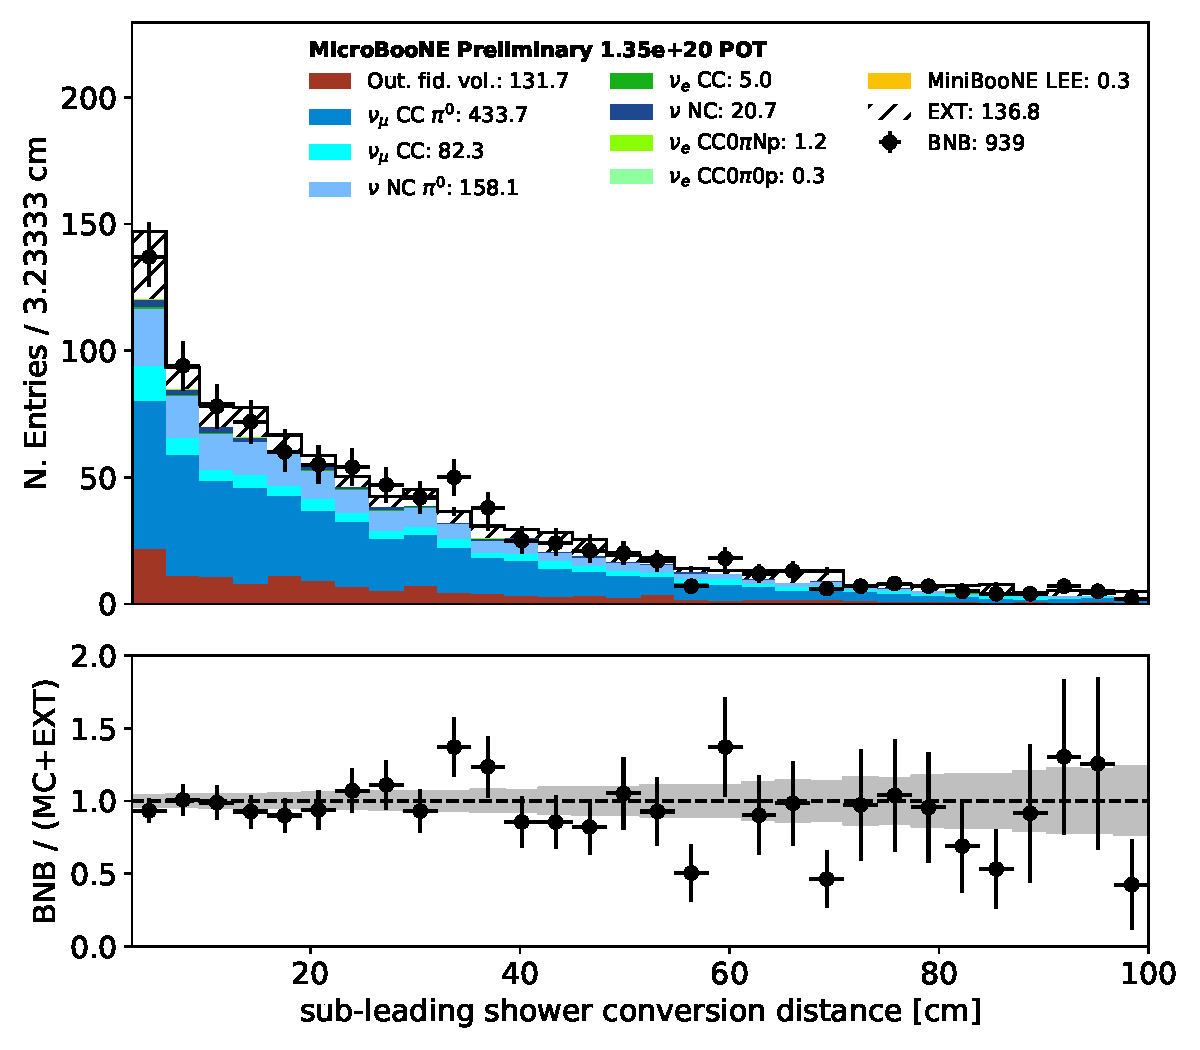
\includegraphics[width=1.00\textwidth]{pi0/pi0_radlen2_01152020_inputs_RUN1.pdf}
    %\caption{\label{fig:pi0:dedx:RUN1:subleading} Run 1 sub-leading shower.}
    \end{subfigure}
    
    \begin{subfigure}[b]{0.38\textwidth}
    \centering
    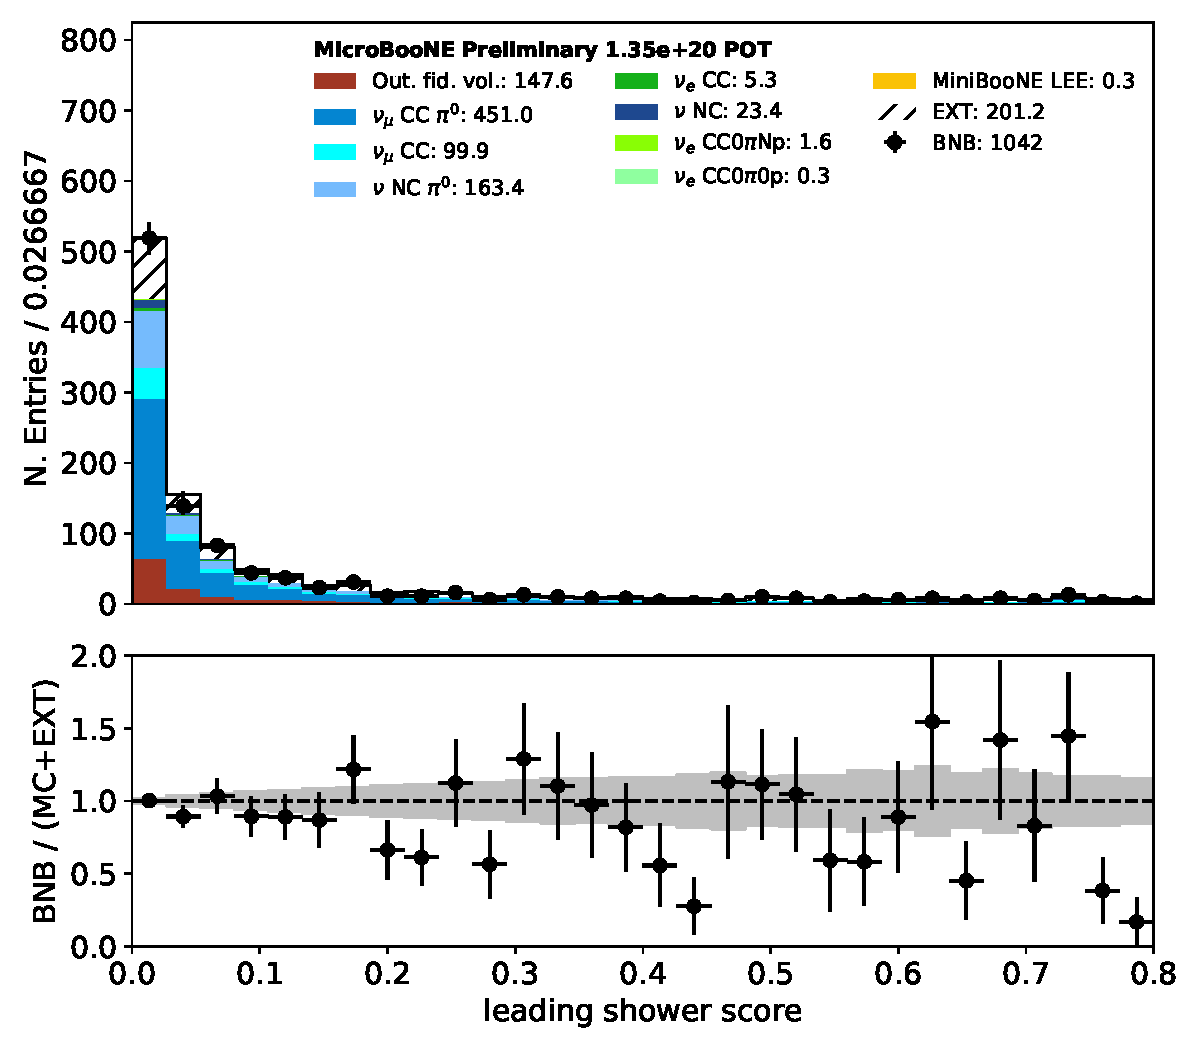
\includegraphics[width=1.00\textwidth]{pi0/pi0_shrscore1_01152020_inputs_RUN1.pdf}
    %\caption{\label{fig:pi0:dedx:RUN1:leading} Run 1 leading shower.}
    \end{subfigure}
    \begin{subfigure}[b]{0.38\textwidth}
    \centering
    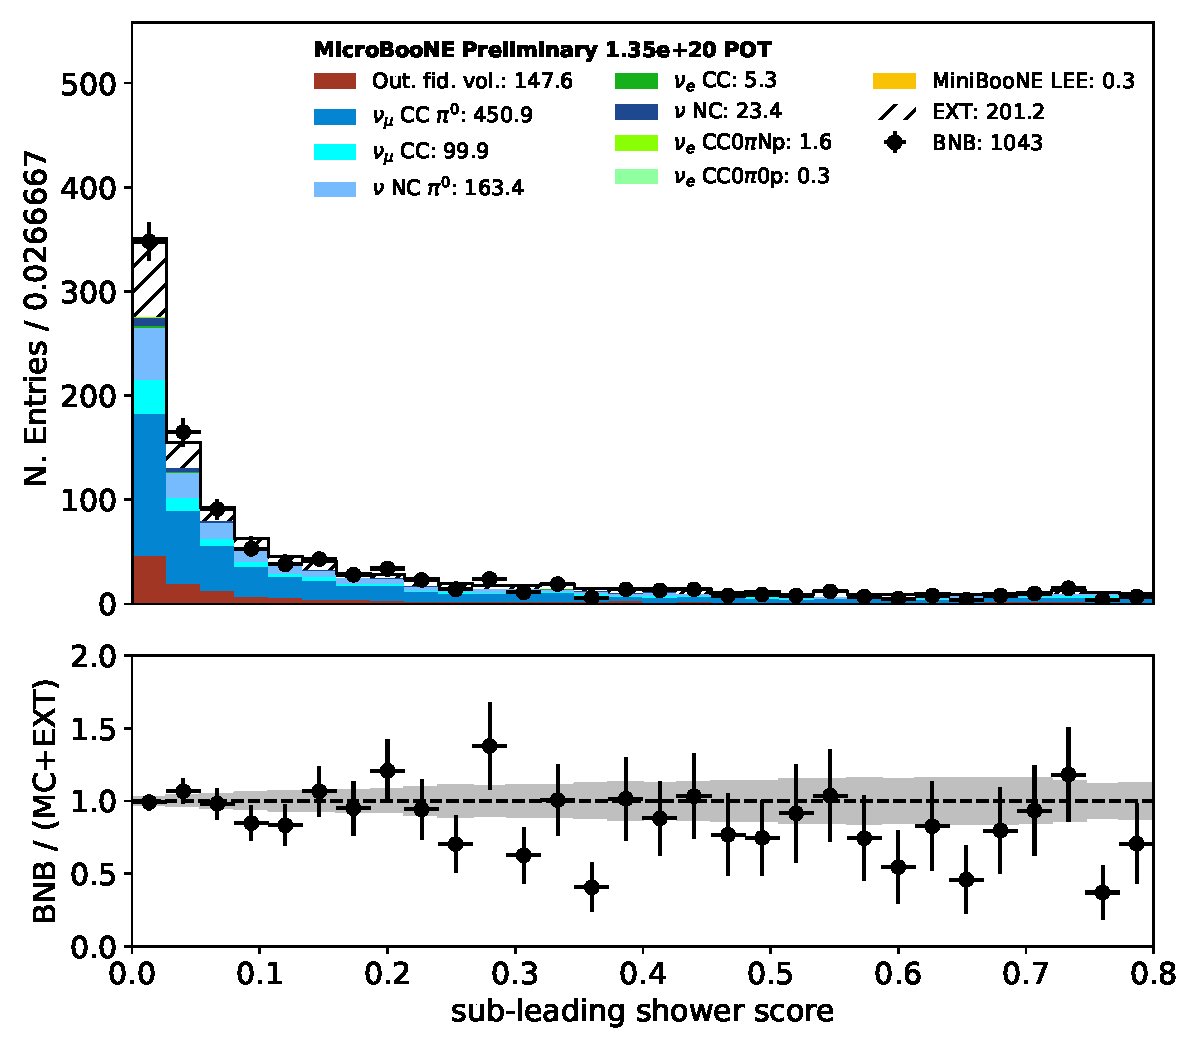
\includegraphics[width=1.00\textwidth]{pi0/pi0_shrscore2_01152020_inputs_RUN1.pdf}
    %\caption{\label{fig:pi0:dedx:RUN1:subleading} Run 1 sub-leading shower.}
    \end{subfigure}
    
    \begin{subfigure}[b]{0.38\textwidth}
    \centering
    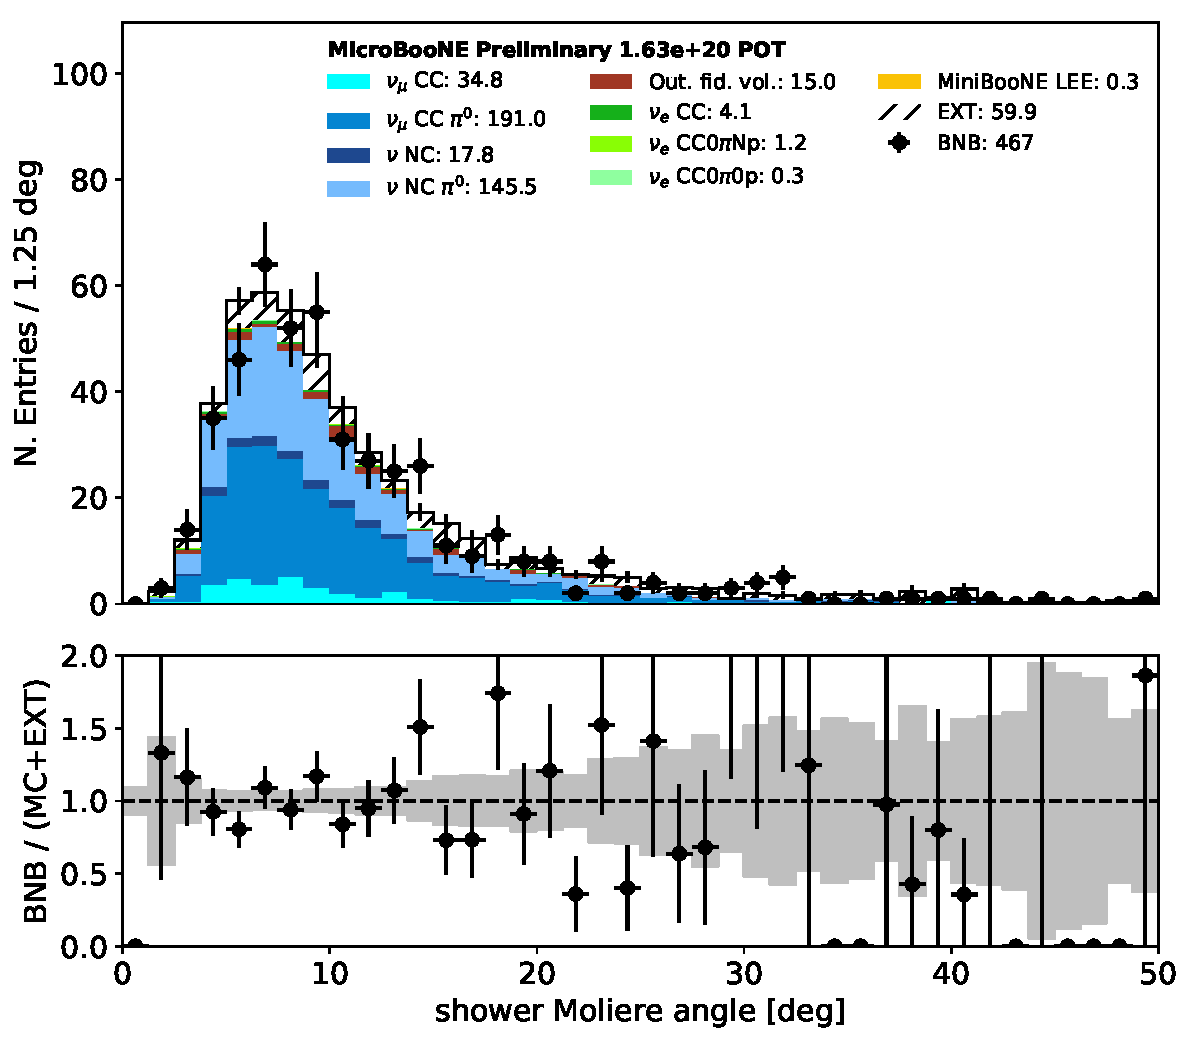
\includegraphics[width=1.00\textwidth]{pi0/shrmoliereavg_01152020_scaled_RUN3.pdf}
    %\caption{\label{fig:pi0:dedx:RUN1:leading} Run 1 leading shower.}
    \end{subfigure}
    \begin{subfigure}[b]{0.38\textwidth}
    \centering
    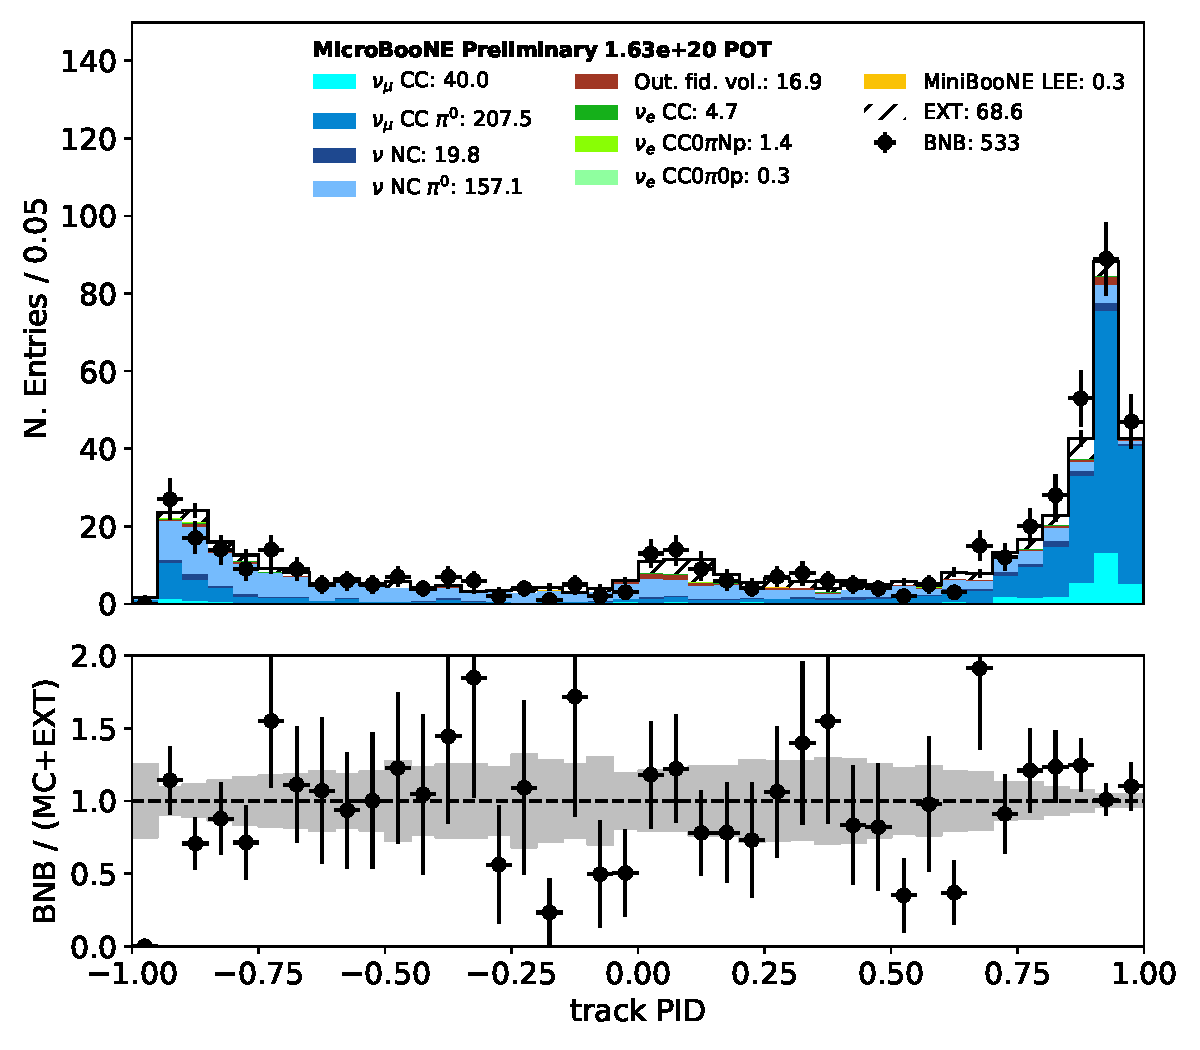
\includegraphics[width=1.00\textwidth]{pi0/trkpid_01152020_scaled_RUN3.pdf}
    %\caption{\label{fig:pi0:dedx:RUN1:subleading} Run 1 sub-leading shower.}
    \end{subfigure}
    
\caption{\label{fig:pi0:datamc}Reconstructed d$E$/d$x$ for leading and sub-leading showers.}
\end{center}
\end{figure}

\subsection{Anti-BDT sample \textcolor{green}{David}}
\par An anti-BDT filter was developed with the goal of isolating $\nu_e$ like backgrounds that could help study in detail data-mc agreement for events that are close to, but not in the $\nu_e$ signal region. The filter selects events that pass the $\nu_e$  pre-selection but fail a past iteration of the 1$e$N$p$ BDT, in order to veto and remain blind to signal events. The filter was run on $1.5E20$ POT of Run 3 data with the goal of studying in particular detail data-mc agreement for Run3, which otherwise would be limited to $0.8E19$ POT of open data. Further documentation on the \emph{anti-BDT} filter is available in reference~\ref{bib:antiBDT}. Comparisons of distributions from this filter are to be made available in a subsequent version of this note.

\newpage

\section{$\nu_e$ Selections}
\par This chapter present the three $\nu_e$ selections which comprise the analysis. The starting point for the $\nu_e$ selections, including a description of efficiencies, are described in section~\ref{sec:nueselection:inputs} . The common variables and tools leveraged for the $\nu_e$ selection are presented in section~\ref{sec:nueselection:variables}. Following sections describe the three channels being targeted: $\nu_e$ inclusive (\ref{sec:nueselection:inclusive}),1$e$N$p$0$\pi$ (\ref{sec:nueselection:1eNp}), and 1$e$0$p$0$\pi$ (\ref{sec:nueselection:1e0p}).

\subsection{Variable definitions \textcolor{red}{Elena}}
\label{sec:nueselection:variables}
\par Variables used for the $\nu_e$ selections aim to isolate features in the neutrino interaction that are specific to events with final-state electrons. These features are split in several categories which leverage calorimetric and topological information that characterizes $\nu_e$ interactions. This section will describe the variables used in the $\nu_e$ selections. Table [\textcolor{red}{TABLE}] summarizes all variables used, with a brief description. Variables that warrant a longer introduction are described below.

\begin{figure}[H]
\begin{center}
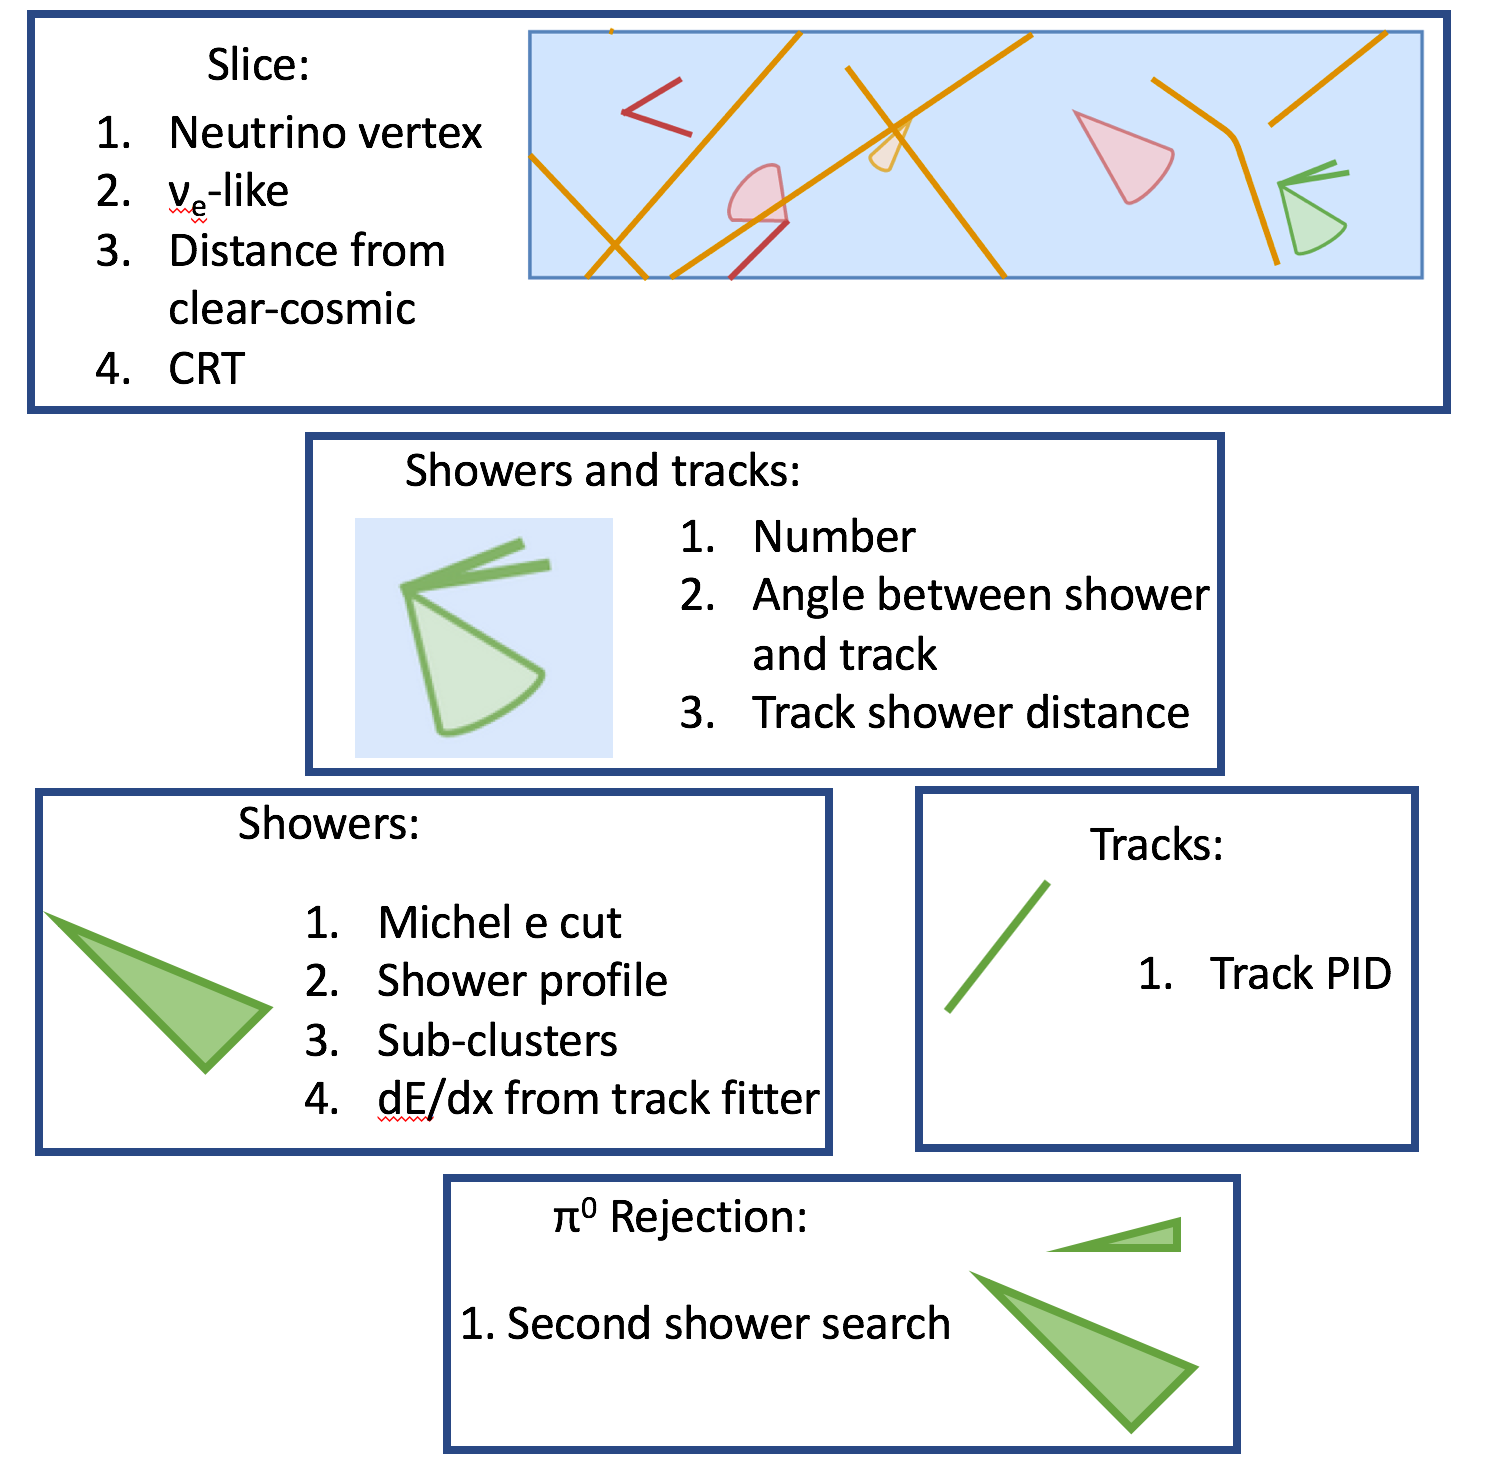
\includegraphics[width=0.6\textwidth]{nueselection/tools.png}
\caption{\label{fig:nue:variables}Categories of variables leveraged in the $\nu_e$ selections.}
\end{center}
\end{figure}

\par \noindent \textbf{track-shower separation} The first step in track-shower separation relies on the topological score reconstructed by Pandora, which utilizes inputs such as the PCA component of 3D space-points to classify PFParticles. Nonetheless, this classification is not sufficient to obtain the track-shower separation needed. To improve on this, additional variables which leverage different aspects of shower topologies are devised:

\begin{itemize}
    \item \textbf{shower track-fitted fraction} (variable: \emph{trkit}, figure~\ref{fig:nue:variables:trkfit}) This quantity is calculated as the fraction of all 3D spacepoints in a shower that are successfully fit with the shower track-fitter algorithm. Tracks, comprised of a single contiguous segment, will be entirely fit, leading to a fraction of 1. Showers, with several branches and split charge deposition segments, will have a fraction that is less then one.
    \item \textbf{shower sub-clusters} (variable: \emph{subcluster}, figure~\ref{fig:nue:variables:subcluster}) This quantity leverages the fact that EM showers are often comprised of several branches isolated by gaps caused by photons propagating through the detector medium. The variable is calculated by counting the number of isolated 2D segments of charge associated to reconstructed showers. This quantity is a sum of such clusters from all three planes.
    \item \textbf{Moliere ``angle''} (variable: \emph{shrmoliereavg}, figure~\ref{fig:nue:variables:dedx}) This quantity aims to characterize the profile of reconstructed EM showers. It is computed using 3D spacepoints. For each 3D spacepoint, the angle between the shower's direction and the spacepoint is calculated. The average of all such angles is used as the variable.
    \item \textbf{dE/dx variables} (variable: \emph{shr\_tkfit\_gap10\_dedx\_\{U,V,Y\}} and \emph{shr\_tkfit\_2cm\_dedx\_\{U,V,Y\}} )  These variables, computed using calorimetric information from each plane. The two different variables are calculated as the median d$E$/d$x$ computed over some segment of a shower's trunk. The two segments used are the first two centimeters, and the range [1,5] cm. The choice to leverage both these variables  is motivated by: (a) Sometimes - especially for the 1$e$0$p$ channel - the first few hits of a shower merge activity from short protons, causing a large d$E$/d$x$ which hampes the ability to identify the event as an electron. (b) For photon showers, especially at low energy, d$E$/d$x$ becomes more and more MIP-like as one moves further along the shower (see figure~\ref{fig:dedxgammas:dist}).
\end{itemize}{}

\begin{figure}[H] 
\begin{center}
    \begin{subfigure}[b]{0.3\textwidth}
    \centering
    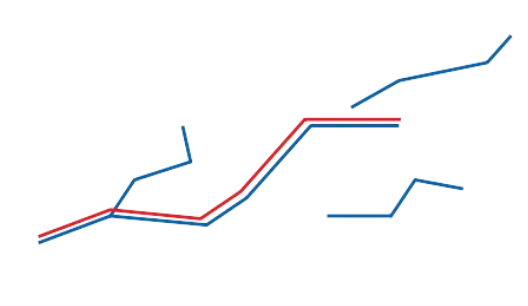
\includegraphics[width=1.00\textwidth]{nueselection/variables/trkfit.png}
    \caption{\label{fig:nue:variables:trkfit} ``trkfit'' variable }
    \end{subfigure}
    \begin{subfigure}[b]{0.3\textwidth}
    \centering
    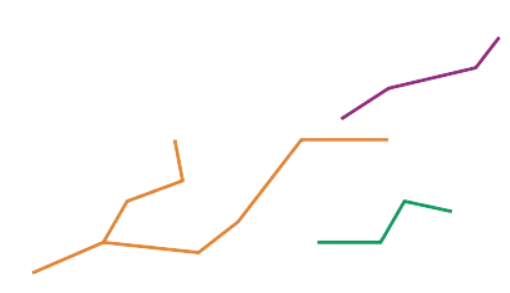
\includegraphics[width=1.00\textwidth]{nueselection/variables/nbranch.png}
    \caption{\label{fig:nue:variables:subcluster} ``subcluster'' variable }
    \end{subfigure}
    \begin{subfigure}[b]{0.3\textwidth}
    \centering
    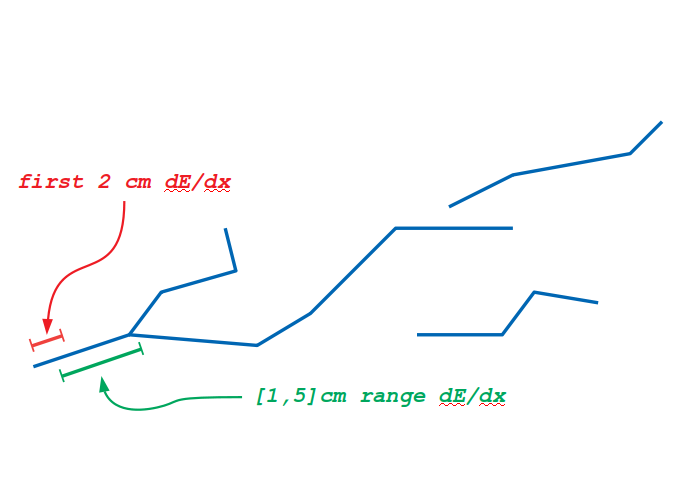
\includegraphics[width=1.00\textwidth]{nueselection/variables/dedx.png}
    \caption{\label{fig:nue:variables:dedx} d$E$/d$x$ variables }
    \end{subfigure}
\caption{\label{fig:nue:presel:eff} Additional shower variables defined by the analysis to improve track-shower separation.}
\end{center}
\end{figure}


\par \noindent \textbf{second-shower variables} Often in $\pi^0$ events one of the two EM $\gamma$ showers is not fully reconstructed by Pandora. In many cases, these second $\gamma$ showers are correctly identified by Pandora as belonging to the neutrino slice (reconstructed in 2D), but never fully reconstructed in 3D (see fig.~\ref{fig:nue:variables:secondshowerevd}). To improve on our $\pi^0$ rejection, we exploit this 2D-only information to reconstruct several variables which store information associated to the largest 2D cluster belonging to the slice on each plane. At the moment, only collection-plane variables are used. The variables, shown graphically in figure~\ref{fig:nue:variables:secondshower}, are described below. In the example event of figure~\ref{fig:nue:variables:secondshowerevd} these quantities are computed for the circles black cluster of charge.
\begin{itemize}
    \item \emph{secondshower\_Y\_nhit}: number of hits in the collection plane of the largest cluster associated to the  recovered 2nd shower
    \item \emph{secondshower\_Y\_dot}: dot product between the vector connecting the vertex to the closest hit in cluster and the charge-weighted cluster direction w.r.t. closest hit in cluster
    \item \emph{anglediff\_Y}: 2D angle difference in the collection plane between the 2nd shower and the 1st shower cluster  (cluster direction defined as charge-weighted direction of cluster w.r.t. vertex)
    \item \emph{secondshower\_Y\_vtxdist}: 2D distance from vertex for the largest 2D cluster associated to the  recovered 2nd shower in the collection plane
\end{itemize}{}

\begin{figure}[H] 
\begin{center}
    \begin{subfigure}[b]{0.35\textwidth}
    \centering
    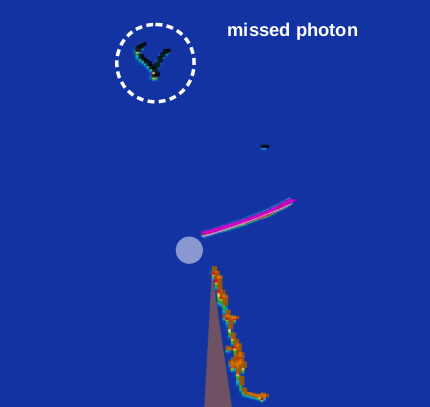
\includegraphics[width=1.00\textwidth]{nueselection/variables/secondshowerevd.png}
    \caption{\label{fig:nue:variables:secondshowerevd} ``trkfit'' variable }
    \end{subfigure}
    \begin{subfigure}[b]{0.35\textwidth}
    \centering
    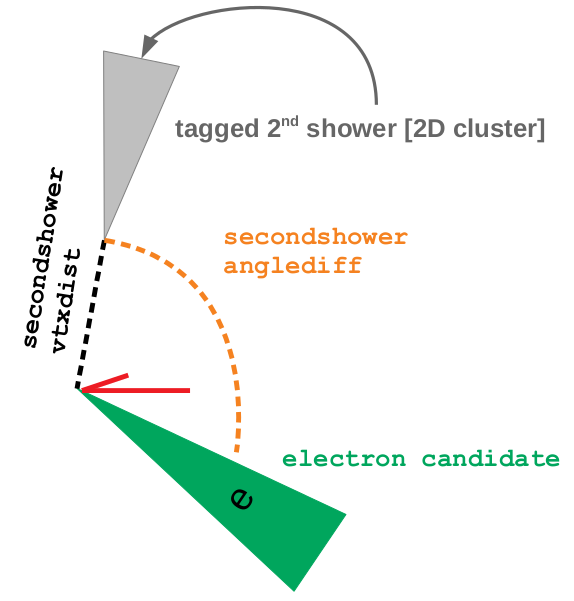
\includegraphics[width=1.00\textwidth]{nueselection/variables/secondshower.png}
    \caption{\label{fig:nue:variables:secondshower} ``subcluster'' variable }
    \end{subfigure}
\caption{\label{fig:nue:variables:secondshower} variables}
\end{center}
\end{figure}

\par \noindent \textbf{track-shower separation} In the 1$e$N$p$ channel, a gap between the shower candidate and vertex activity is a powerful $\pi^0$ rejection discriminant. We primarily rely on the measured 3D distance between the shower start point and the reconstructed start point of the longest track in the slice (variable: \emph{tksh\_distance}). Due to mis-reconstruction in the 3D shower and track reconstruction, sometimes the 3D distance just defined is reconstructed to be large (up to several centimeters) even if the individual track and shower are correctly clustered. This factors smears the track-shower separation of $\nu_e$ interactions therefore reducing the $e-\gamma$ separation power achievable. To overcome this failure specific to the 3D reconstruction, a new quantity is calculated with 2D information from the collection plane defined as the smallest 2D distance between any hits associated with the shower candidate and any hits associated with the proton candidate.


\par \noindent  \textbf{Slice variables}: these are variables associated to general features of the reconstructed neutrino interaction or event.

\begin{itemize}
    \item \emph{nslice}: number of neutrino slices identified by the SliceId (possible values are 0 and 1);
    \item \emph{reco\_nu\_vtx\_sce\_\{x,y,z\}}: Reconstructed space charged corrected neutrino interaction vertex in (x,y,z) coordinates.
    \item \emph{n\_showers\_contained}: number of showers with a starting point within the fiducial volume;
    \item \emph{n\_tracks\_contained}: number of tracks fully contained in the fiducial volume;
    \item \emph{contained\_fraction}: fraction of hits in PFParticles contained in the fiducial volume (according to definitions above) with respect to the total number of clustered hits in the slice;
    \item \emph{hits\_ratio}: ratio between hits from showers and total number of hits;
    \item \emph{CosmicIP}: closest distance between shower start and space points associated to tracks flagged as cosmics.
    \item \emph{crtveto}: boolean variable checking whether the event passes the CRT veto or not
    \item \emph{\_closestNuCosmicDist}: minimum 3D distance of the reconstructed neutrino vertex from a CRT-tagged cosmic track
    \item \emph{slclustfrac}: fraction of hits in the slice that are fully reconstructed to 3D particles.
\end{itemize}

\par \noindent \textbf{Shower and Track variables}:

\begin{itemize}
    \item \emph{tksh\_distance}: distance between leading shower vertex and longest track vertex;
    \item \emph{tksh\_angle}: angle between leading shower vertex and longest track vertex;
    item \emph{merge\_bestdist}: Distance between shower start point and track start (or end) point for the track in the slice that best matches the direction of the shower. 
\end{itemize}

\par \noindent \textbf{Shower variables}:

\begin{itemize}
    \item \emph{shr\_energy\_tot\_cali}: sum of the energy of the calibrated showers (in GeV). This variable is used only at pre-selection as a ``Michel veto'';
    \item \emph{shr\_tkfit\_2cm\_dedx\_\{U,V,Y\}}: dE/dx in the first 2 cm of the leading shower on plane (U,V,Y) with the track fitting;
    \item \emph{shr\_tkfit\_gap10\_dedx\_\{U,V,Y\}}: dE/dx in the [1,5] cm range of the leading shower on plane (U,V,Y) with the track fitting;
    \item \emph{shr\_score}: Pandora SVM track/shower score for the leading shower;
    \item \emph{shrmoliereavg}: average angle between the vector connecting the shower start to each shower space point and the shower direction vector
    \item \emph{subcluster}: number of subclusters (counted in all planes) for the leading shower.
    \item \emph{trkfit}: ratio of hits fitted in the track fit to the shower to all hits in the shower.
\end{itemize}

\par \noindent  \textbf{Track variables}:

\begin{itemize}
    \item \emph{trkpid}: proton-muon LLR particle identification 
\end{itemize}

\par \noindent  \textbf{2nd shower-based $\pi^0$ rejection variables}:

\begin{itemize}
    \item \emph{secondshower\_Y\_nhit}: number of hits in the collection plane of the largest cluster associated to the  recovered 2nd shower
    \item \emph{secondshower\_Y\_dot}: dot product between the vector connecting the vertex to the closest hit in cluster and the charge-weighted cluster direction w.r.t. closest hit in cluster
    \item \emph{anglediff\_Y}: 2D angle difference in the collection plane between the 2nd shower and the 1st shower cluster  (cluster direction defined as charge-weighted direction of cluster w.r.t. vertex)
    \item \emph{secondshower\_Y\_vtxdist}: 2D distance from vertex for the largest 2D cluster associated to the  recovered 2nd shower in the collection plane
\end{itemize}


\clearpage
\subsection{$\nu_e$ CC Inclusive selection \textcolor{red}{Wouter}}
\label{sec:nueselection:inclusive}


\newcommand{\nueccinc}{$\nu_e$ CC inclusive\xspace}
\newcommand{\nueccsel}{$\nu_e$ CC inclusive selection\xspace}


The aim of the inclusive charged-current electron neutrino selection is to select electron neutrinos independently of their final state and energy. The selection efficiency is approximately 20\%, leading to 250-300 electron neutrino's in the Run 1-4 data-set. The purity without CRT is $\approx 35-40\%$ and with CRT $\approx 45-50\%$.

\subsubsection{Pre-selection}
The selection builds on top of the SliceID (\cref{sec:sliceID}). At the preselection stage,  the cuts listed in \cref{tab:nuecc:presel} are applied. %Here, an electron candidate shower is defined as a particle with a \textit{track\_score} below 0.3, and hits on all three planes. Furthermore, a minimum calorimeric energy of \SI{75}{\MeV} is required. 
\begin{comment}
\begin{table}[h!]
\centering
\setlength{\tabcolsep}{10pt}
\renewcommand{\arraystretch}{1.25}
 \begin{tabular}{| c | c |} 
 \hline
 Cut goal & Cut definition \\
 \hline\hline
Signal topology & An electron candidate shower \\
 \hline
\multirow{2}{*}{Cosmic rejection} & topological\_score $>$ 0.15 \\
 & CosmicIP $>$ $\SI{15}{\cm}$ \\
 \hline
Fiducial volume & \makecell{Reconstructed, space-charge corrected vertex \\ inside a volume defined by borders of \\ \SI{10}{\cm} in $x$ and $y$ and $[ \SI{20}{\cm}, \SI{50}{\cm}]$ in $z$} \\
 \hline
Reconstruction quality & \textit{slclustfrac} $>$ 0.4 \\
\hline
Electron Candidate &  track\_score $<$ 0.3, hits in all three planes \\
\hline
Michel rejection & shr\_energy\_tot\_cali $>$ 0.075 GeV \\
 \hline
 \end{tabular}
 \caption{\label{tab:nuecc:presel} Preselection requirements for the \nueccsel.  }
\end{table}
\end{comment}
At this stage, the efficiency of the selection is 46\% for $\nu_e$ CC events inside the fiducial volume\textcolor{blue}{Do we have the plot of efficiency as a function of true nu E? }. This is equivalent to 618 events per \SI{10.1e20}{POT}. The number of LEE signal events passing is approximately 30 per \SI{10.1e20}{POT}. The purity at this stage is $\sim$3.0\%. 

After the pre-selection cuts, the $\nu_e$ CC purity is still low. Figure \ref{fig:pre_shower_E_pdg} shows the distribution of the angles of the electron candidate shower highlighting the dominant background categories: the main background is coming from events with $\pi^0$ in the final state. Thus, $e/\gamma$ separation becomes key to the $\nu_e$ CC inclusive selection.

\cref{fig:e_cand_Calo} shows the agreement in the kinematics of the electron candidate shower at the pre-selection stage. \emph{As seen in several other Data-MC comparisons of calorimetry variables throughout this note, a slight disagreement is found in the shower candidate energy, to be re-evaluated after the planned MC re-calibration.}


\begin{figure}[h]
    \centering
    \includegraphics[height=4.9cm]{NueCCsel/Images/run1/pre_angles.pdf}
    \caption{MC-Data comparison of the angles of the electron candidate after the pre-selection cuts.}
    \label{fig:pre_shower_E_pdg}
\end{figure}

\begin{figure}[h]
    \centering
     \includegraphics[height=4.9cm]{NueCCsel/Images/run1/pre_shower_E_pdg.pdf}
    \includegraphics[height=4.9cm]{NueCCsel/Images/run1/e_cand_dedxColl}
    \caption{ Energy (\emph{Left}) of the electron candidate after the pre-selection cut d$E$/d$x$ on the collection plane (\emph{Right}) of the electron candidate shower after the pre-selection.}
    \label{fig:e_cand_Calo}
\end{figure}


\subsubsection{Electron Identification}
After the pre-selection, the object that is tagged as electron candidate is still not an neutrino electron in the dominant fraction of events. The ratio photons to electrons is approximately 20 to 1 and photon-electron separation is therefore the main objective of electron identification. The identification is done using a boosted decision tree, trained on variables characterizing the particle. 

Even if a number of variables contribute to the BDT (see backup \ref{sec:datamc:nueccinclusive}),  we highlight here some distributions which show the cleanest e/$\gamma$: separation: the  d$E$/d$x$ distribution on  collection plane (left side of Figures \ref{fig:e_cand_Calo}), the shower vertex distance and average molier radius (\cref{fig:e_cand_dist} left and center) . The response of the BDT is shown in the right panel of \cref{fig:e_cand_dist}. The complete list of variables used to train the BDT for electron identification is: \emph{shower\_vtx\_dist}, \emph{nObjHits\_Y},  \emph{shr\_tkfit\_2cm\_dedx\_Y},  \emph{shr\_tkfit\_2cm\_dedx\_ALL},  \emph{shr\_tkfit\_gap10\_dedx\_Y}, \emph{shrmoliereavg}, \emph{secondshower\_Y\_vtxdist}, \emph{subcluster}, \emph{ismerged}.

\begin{comment}
 Those variables are listed in \cref{tab:nuecc:e_bdt}.

\begin{table}[h!]
\centering
\setlength{\tabcolsep}{10pt}
\renewcommand{\arraystretch}{1.25}
\begin{tabular}{| c | c |} 
\hline
Cut goal & Cut definition \\
\hline\hline
\multirow{2}{*}{$e/\gamma$ separation} & Shower vertex distance \\
                                       & \makecell{Shower d$E$/d$x$ at the start of the shower: \\
                                            \tabitem On the collection plane only.\\
                                            \tabitem Weighted mean over the 3 planes.\\
                                            \tabitem Collection plane, but shifted by \SI{1}{\cm}.\\ 
                                            }\\
\hline
\multirow{2}{*}{$\pi^0$ tagging} & \textit{secondshower\_Y\_nhit} \\
 & \textit{secondshower\_Y\_vtxdist} \\
 \hline
\multirow{2}{*}{$\mu$-rejection} & \textit{shrmoliereavg} \\
                                 & \textit{subcluster} \\
 \hline
Reconstruction quality & \makecell{\textit{ismerged} \\ Checks if a proton is merged in the start of the shower. } \\
 \hline
 \end{tabular}
 \caption{\label{tab:nuecc:e_bdt} Input variables used by the BDT to do electron identification.}
\end{table}
\end{comment}


\begin{figure}[h]
    \centering
    \includegraphics[height=5cm]{NueCCsel/Images/run1/e_cand_dist.pdf}
    \includegraphics[height=5cm]{NueCCsel/Images/run1/pre_e_score.pdf}
    \caption{The left two panels show important variables to identify electrons after the pre-selection. The right panel shows the BDT electron identification response, demonstrating a good e/$\gamma$ separation.}
    \label{fig:e_cand_dist}
\end{figure}

%\begin{figure}
%    \centering
%    \includegraphics[width=\textwidth]{NueCCsel/Images/run1/e_cand_subclusters.pdf}
%    \caption{Caption}
%    \label{fig:e_cand_subclusters}
%\end{figure}

%\begin{figure}
%    \centering
%   \includegraphics[width=\textwidth]{NueCCsel/Images/run1/e_cand_secondshower.pdf}
%    \caption{Caption}
%    \label{fig:e_cand_secondshower}
%\end{figure}

\subsubsection{Other Daughters Identification}
Besides the electron candidate, the slice includes a number of particles which can be leveraged to improve background rejection. We classify each PFParticle using the ``other-daughters-BDT". This BDT is trained on three labeled categories: \emph{signal-like}, \emph{neutral}, \emph{background-like}. The signal-like particles are those PFParticles that are backtracked to a proton or a split-off part of the electron associated to $\nu_e$ interactions: we want to keep events with a high content of signal-like particles. The background-like particles are those PFParticles that are backtracked to a simulated muon or cosmic activity.
The ``neutral" label accounts for tricker cases: this label is given to PFParticles backtracked to charged pions or photons. Charged pions should be allowed in a $\nu_e$ CC search, but the mis-identification rate between charged pions and muons is large in LArTPCs. Photons coming from neutral pions are allowed in a  $\nu_e$ CC inclusive search, but they can also constitute a pernicious background.

The input variables of the other-daughters-BDT are listed in \cref{tab:nuecc:other_bdt}.
The three most important distributions of the variables used are given in \cref{fig:pre_daughter_1}.  


The response of the other-daughters-BDT is a score assigned to each PFParticle, whose distribution is shown in \cref{fig:pre_daughter_score}: high scores classify the PFParticles as signal-like. 

For each event, we create two important variables that inform the event selection starting from this BDT output:  \emph{otherD\_MeanScore} and \emph{otherD\_LowestScore}.  The variables \emph{otherD\_MeanScore} and   \emph{otherD\_LowestScore} are the average and the lowest other-daughters-BDT score calculated using all the PFParticles in the event that are not the electron. Both the  \emph{otherD\_MeanScore} and  \emph{otherD\_LowestScore}  is assigned the default value 1 in the case the event is made of just the single electron shower.


\begin{table}[h!]
\centering
\setlength{\tabcolsep}{10pt}
\renewcommand{\arraystretch}{1.25}
\begin{tabular}{| c | c |} 
\hline
Cut goal & Cut definition \\
\hline\hline
\multirow{3}{*}{particle identification} & \textit{trk\_llr\_pid\_score} \\
                                         & \textit{trk\_distance} \\
                                         & \textit{trk\_score}\\
\hline
\multirow{2}{*}{particle hierarchy} & \textit{pfp\_generation} \\
                                    & \textit{Number of daughters of the particle} \\

 \hline
 \end{tabular}
 \caption{\label{tab:nuecc:other_bdt} Input variables used by the BDT to classify the other daughter particles.}
\end{table}



\begin{figure}
    \centering
    \includegraphics[width=\textwidth]{NueCCsel/Images/run1/pre_daughter_1.pdf}
    \caption{Variables used to identify the other daughters of the neutrino besides the electron candidate shower. The distributions include all non-electron tagged daughters after the pre-selection.}
    \label{fig:pre_daughter_1}
\end{figure}

%\begin{figure}
%    \centering
%    \includegraphics[width=\textwidth]{NueCCsel/Images/run1/pre_daughter_2.pdf}
%    \caption{Caption}
%    \label{fig:pre_daughter_2}
%\end{figure}

\begin{figure}
    \centering
    \includegraphics[width=0.5\textwidth]{NueCCsel/Images/run1/pre_daughter_score.pdf}
    \caption{BDT response to classify the non-electron candidate daughters in the event. The cosmogenic particles, together with the muons and photons have a low response, indicating higher likeliness to be background. The protons have a high response on the right.}
    \label{fig:pre_daughter_score}
\end{figure}

\subsubsection{Event Selection}
We construct the final event classification BDT building on the particle identification performed in the two previous sections. For this final BDT, the dominating variable is the electron identification response but the full list of variables is, in sequence of importance:

\begin{enumerate}
    \item electron BDT response
    \item otherD\_LowestScore
    %\textcolor{blue}{(David) Lowest means the score for the least nue-like PFParticle? What happens if no additional PFParticle is present?}
    \item contained\_fraction
    \item number of showers
    \item hits\_ratio
    \item otherD\_MeanScore
    \item number of particles in the slice that have a reconstructed start point more than \SI{3}{\cm} from the neutrino vertex.
\end{enumerate}
The response of the event classification is given in the left panel \cref{fig:pre_event_score}. After the selection, the efficiency is 21\%, corresponding to 280 electron neutrino's in the Run 1-4 data-set. The distribution of the reconstructed electron energy is given in the right panel of \cref{fig:pre_event_score}. \cref{fig:nueccinc_eff} documents the efficiency of the SliceID, pre-selection and final inclusive selection for the three final state categories \textcolor{blue}{In the context of this note, I think it would be better to have the combined efficiency of the three channels (cause otherwise the reader can get confused with the previous sections)}.

%\begin{figure}
%    \centering
%    \includegraphics[width=\textwidth]{NueCCsel/Images/run1/bdt_1.pdf}
%    \caption{Caption}
%    \label{fig:bdt_1}
%\end{figure}

%\begin{figure}
%    \centering
%    \includegraphics[width=\textwidth]{NueCCsel/Images/run1/bdt_2.pdf}
%    \caption{Caption}
%    \label{fig:bdt_2}
%\end{figure}

\begin{figure}
    \centering
    \includegraphics[width=0.445\textwidth]{NueCCsel/Images/run1/pre_event_score.pdf}
    \includegraphics[width=0.545\textwidth]{NueCCsel/Images/run1/nue_shower_energy_y.pdf}
    \caption{(left) BDT response of the $\nu_e$ CC inclusive event classifier. (right) Electron shower energy distribution after the selection.}
    \label{fig:pre_event_score}
\end{figure}

\begin{figure}
    \centering
    \includegraphics[width=\textwidth]{NueCCsel/Images/run1/efficiency_cat_2.pdf}
    \caption{Efficiency of the different stages in the selection in function of the true neutrino energy. The different panels correspond to different final states of interest.}
    \label{fig:nueccinc_eff}
\end{figure}


\clearpage



\subsection{Input to \npsel and \opsel and channel orthogonality \textcolor{green}{David + Sophie}}
\label{sec:nueselection:inputs}

The 1$e$N$p$ and 1$e$0$p$ selections rely on a common pre-selection which requires the presence of at least one reconstructed and contained EM shower (figure~\ref{fig:nue:presel:nshower}) with reconstructed energy above 70 MeV (figure~\ref{fig:nue:presel:shrenergy}). This second cut applies as a Michel-electron veto, as the majority of events which do not pass this cut are associated to cosmic or $\nu_{\mu}$ induced $\mu \rightarrow e$ Michel electrons. The two selections are subsequently split based on whether a proton candidate is (N$p$) or is not (0$p$) found. Events with a fully contained track must have a \texttt{trkpid} score $< 0$ and a value of \texttt{tksh\_angle} $> -0.9$. The first condition requires that the track be proton-like according to the PID tool~\ref{subsec:loglikelihoodpid}, while the second excludes tracks reconstructed back-to-back to the electron candidate, generally due to mis-reconstruction. For events with more than one reconstructed track, these requirements are applied on the longest track.

\begin{figure}[H] 
\begin{center}
    \begin{subfigure}[b]{0.3\textwidth}
    \centering
    \includegraphics[width=1.00\textwidth]{nueselection/n_showers_contained_01132020_RUN1.pdf}
    \caption{\label{fig:nue:presel:nshower} }
    \end{subfigure}
    \begin{subfigure}[b]{0.3\textwidth}
    \centering
    \includegraphics[width=1.00\textwidth]{nueselection/n_tracks_contained_01132020_RUN1.pdf}
    \caption{\label{fig:nue:presel:ntrack} }
    \end{subfigure}
    \begin{subfigure}[b]{0.3\textwidth}
    \centering
    \includegraphics[width=1.00\textwidth]{nueselection/shr_energy_tot_cali_01132020_RUN1.pdf}
    \caption{\label{fig:nue:presel:shrenergy} }
    \end{subfigure}
\caption{\label{fig:nue:presel}Variables input to the common $\nu_e$ N$p$ and 0$p$ pre-selections.}
\end{center}
\end{figure}

\par The efficiencies of the 1$e$N$p$ and 1$e$0$p$ channels at the point where the selections diverge are shown in figure~\ref{fig:nue:presel:eff}. Efficiencies are presented as a function of true neutrino energy~\ref{fig:nue:presel:eff:nu}, proton KE~\ref{fig:nue:presel:eff:proton}, and electron energy~\ref{fig:nue:presel:eff:elec}. Each plot shows in black the efficiency for the common pre-selection (before a proton requirement is or is not imposed) and is reported relative to all intrinsic $\nu_e$ events. In blue and red respectively are shown the efficiencies for the  1$e$N$p$ and 1$e$0$p$ selections respectively, relative to true N$p$ and 0$p$ events. Shaded histograms in red and blue show the stacked truth-level distributions for N$p$ and 0$p$ events for the variables being plotted. An important observation to make is the fact that at this pre-selection stage the efficiency for 1$e$N$p$ events is significantly lower then that of 1$e$N$p$ events. This is caused by the additional requirement of the presence of a proton-like track in the final state. The strong energy dependence for the efficiency in tagging protons is shown in figure~\ref{fig:nue:presel:eff:proton}. While requiring the presence of a final-state proton lowers the efficiency, this requirement has a significant impact on the selection's ultimate purity.

\begin{figure}[H] 
\begin{center}
    \begin{subfigure}[b]{0.3\textwidth}
    \centering
    \includegraphics[width=1.00\textwidth]{nueselection/nu_RUN1.pdf}
    \caption{\label{fig:nue:presel:eff:nu} }
    \end{subfigure}
    \begin{subfigure}[b]{0.3\textwidth}
    \centering
    \includegraphics[width=1.00\textwidth]{nueselection/proton_RUN1.pdf}
    \caption{\label{fig:nue:presel:eff:proton} }
    \end{subfigure}
    \begin{subfigure}[b]{0.3\textwidth}
    \centering
    \includegraphics[width=1.00\textwidth]{nueselection/elec_RUN1.pdf}
    \caption{\label{fig:nue:presel:eff:elec} }
    \end{subfigure}
\caption{\label{fig:nue:presel:eff} $\nu_e$ pre-selection efficiencies split by final-state topology as a function of different truth variables.}
\end{center}
\end{figure}

\subsection{\npsel Channel \textcolor{red}{David + Giuseppe}}
\label{sec:nueselection:1eNp}

The 1$e$N$p$ channel is the most sensitive to the MiniBooNE eLEE signal as it contains a large fraction of the signal events and allows for selection requirements based both on showers and tracks. 
Given the large cosmic background and that $\nu_e$ charge-current interactions are O(1\%) in the BNB, a high-purity selection is needed to achieve a sizeable signal sensitivity; the necessary trade-off is that the final signal efficiency will be low.

The section is organized as follows. We first define a set of minimal requirements ("preselection") to obtain a high statistics sample (dominated by cosmic and neutrino backgrounds) that is used to monitor the data-MC agreement of the selection variables. We then define two alternative selections, respectively based on a simple box-cut approach and on boosted decision trees (BDT); the BDT approach is expected to be the most sensitive, while box-cuts provide a robust reference selection. Finally we compare all presented selections in terms for their signal efficiency and purity.

\subsubsection{Preselection}

At preselection stage we apply the minimum set of requirements so that all selection variables can be defined, plus the containment and a minimum shower energy to reject Michel electrons:
\begin{itemize}
    \item nslice = 1
    \item n\_tracks\_contained $>$ 0
    \item n\_showers\_contained $>$ 0
    \item contained\_fraction $>$ 0.9
    \item shr\_energy\_tot\_cali $>$ 0.07
\end{itemize}

The relative fraction of EXT events at this stage is roughly 25\%, so we can look at all selection variables in data and MC in a neutrino-dominated sample with the open Run1 and Run3 data sets. We typically see very good agreement, which rules out major problems related to POT-scaling, detector modeling, inclusive cross-section. The full list of plots can be found in Appendix~\ref{sec:datamc:plots}. Figure~\ref{fig:1eNp:prsel} shows the level of agreement for the reconstructed neutrino energy variable. \textcolor{red}{We should probably discuss variables with not so great data-MC agreement here (in case they are not already discussed elsewhere).}

\begin{figure}[ht] 
\begin{center}
    \begin{subfigure}[b]{0.45\textwidth}
    \centering
    \includegraphics[width=1.00\textwidth]{1eNp/reco_e_01162020_RUN1.pdf}
    \caption{\label{fig:1eNp:prsel:RUN1} RUN 1}
    \end{subfigure}
    \begin{subfigure}[b]{0.45\textwidth}
    \centering
    \includegraphics[width=1.00\textwidth]{1eNp/reco_e_01162020_RUN3.pdf}
    \caption{\label{fig:1eNp:prsel:RUN1} RUN 3}
    \end{subfigure}
\caption{\label{fig:1eNp:prsel}Reconstructed neutrino energy after pre-selection for the \npsel channel.}
\end{center}
\end{figure}

\subsubsection{Box-cuts}

On top of preselection requirements we define a robust selection based on box cuts targeting high $\nu_e$ purity, especially at lower energy.
In this section cuts are presented in different categories according to the background they primarily suppress; however, to the extent that some variables are effective against multiple backgrounds, the following description should be regarded as a simplification.

First, we aim at rejecting cosmic-induced events by requiring a large distance of the neutrino vertex from clear cosmic tracks and a proton-like track. The latter requirement in particular rejects more than 90\% of the cosmics that pass pre-selection. The next goal is to suppress events from $\nu_\mu$ charged current interactions, so for this purpose we require shower hits to be the dominant in the slice, as well as imposing tight quality requirements on the shower object. They rely on several variables aiming at separating electron or photon showers from single-particle tracks, i.e. shr\_score, shrmoliereavg, trkfit, subcluster. 

At this stage most of the selected events contain neutrino-induced electromagnetic activity. The main background are $\pi^0$ events abd we reject them with a series of requirements based on the different topology and energy deposition of electrons and photons. We first require only one shower-like PFParticle in the event, and that its start point is at a short distance from the track start. Then, we require that the energy loss at the start of the electron shower is be compatible with a single MIP. Many possible dEdx variable definitions are possible, and information from all TPC planes can be used. However, due to detector and reconstruction limitations, there is not a single definition that provides a sharp separation between electrons and photons; therefore, in order to obtain a good background rejection without large efficiency losses, we choose to apply a loose MIP cut on two different dEdx definitions (described in Sec.~\ref{sec:nueselection:variables}). The loose MIP requirement enforces that there is at least one hit in the collection plane in the probed range, and that the dEdx is not consistent with two or more MIPs in any plane. Finally, the single shower requirement is reinforced with a 2nd shower veto based on clusters in the collection plane that are not matched to any PFParticle.

The last cut aims at rejecting misreconstructed events, so when the track and shower are aligned the candidate event is rejected.

For reference, the full list of cuts is:
\begin{itemize}
    \item CosmicIP $>$ 20.
    \item trkpid $<$ -0.02
    \item hits\_ratio $>$ 0.60
    \item shr\_score $<$ 0.275
    \item shrmoliereavg $>$ 2 and shrmoliereavg $<$ 9
    \item trkfit $<$ 0.45 or subcluster $>$ 6
    \item n\_showers\_contained = 1
    \item tksh\_distance $<$ 3.5
    \item shr\_tkfit\_2cm\_dedx\_Y $\in$ [0,4.0] and shr\_tkfit\_2cm\_dedx\_U $<$ 4.0 and shr\_tkfit\_2cm\_dedx\_V $<$ 4.0
    \item shr\_tkfit\_gap10\_dedx\_Y $\in$ [0,4.5] and shr\_tkfit\_gap10\_dedx\_U $<$ 4.5 and shr\_tkfit\_gap10\_dedx\_V $<$ 4.5
    \item secondshower\_Y\_nhit $\leq$ 8 or secondshower\_Y\_dot $\leq$ 0.8 or anglediff\_Y $\leq$ 40 or secondshower\_Y\_vtxdist $\geq$ 100
    \item tksh\_angle $>$ -0.9 and tksh\_angle $<$ 0.7
\end{itemize}

\par 
Topics to discuss: selection efficiency and purity, expected number of events in open data and in full sample.

\begin{figure}[ht]
\begin{center}
\includegraphics[width=0.45\textwidth]{1eNp/reco_e_01162020_box_RUN1.pdf}
\caption{\label{fig:1eNp:box:RUN1}Box-cuts for \npsel channel.}
\end{center}
\end{figure}

\begin{figure}[H] 
\begin{center}
    \begin{subfigure}[b]{0.45\textwidth}
    \centering
    \includegraphics[width=1.00\textwidth]{1eNp/1eNp_box_evd1.png}
    \caption{\label{fig:1eNp:box:evd1}1.19 GeV [reco] $\nu_e$ candidate}
    \end{subfigure}
    \begin{subfigure}[b]{0.45\textwidth}
    \centering
    \includegraphics[width=1.00\textwidth]{1eNp/1eNp_box_evd2.png}
    \caption{\label{fig:1eNp:box:evd2}1.15 GeV [reco] $\nu_e$ candidate}
    \end{subfigure}
\caption{\label{ffig:1eNp:box:evd} \npsel candidates from the open $4eE19$ Run1 open dataset. Two data events are found when }
\end{center}
\end{figure}

\subsubsection{BDT}

Two BDTs are trained separately to reject backgrounds with and without $\pi^0$ in the final state. The same set of training variables is used in the two BDTs, corresponding to the list of variables used in the box-cut selection. 

Both in the training and in the analysis, events are required to pass the preselection requirements plus a loose set of cuts intended to avoid considering events where one or more variables is clearly inconsistent with $\nu_e$ events. The list of cuts is:
\begin{itemize}
    \item CosmicIP $>$ 20.
    \item trkpid $<$ 0.1
    \item hits\_ratio $>$ 0.5
    \item shr\_score $<$ 0.30
    \item n\_showers\_contained = 1
    \item tksh\_distance $<$ 6.0
    \item shr\_tkfit\_2cm\_dedx\_Y $<$ 4.0
    \item tksh\_angle $>$ -0.9
\end{itemize}

\begin{figure}[H]
\begin{center}
\includegraphics[width=0.45\textwidth]{1eNp/loose_sel_perf.png}
\caption{\label{fig:1eNp:loosesel} Fraction of events in the BNB sample divided in different categories before and after the loose selection.}
\end{center}
\end{figure}

Indeed the BDT is able to figure out during training which variables are most important for each background: shower quality variables (e.g. shr\_score, trkfit, subcluster) have higher ranking for the non-$\pi^0$ BDT, while variables such as tksh\_distance and the shower dEdx show higher importance for the $\pi^0$-BDT. It is interesting to note that the most discriminating variable is in both cases shrmoliereavg which may be useful to discriminate both muons in $\nu_\mu$ events (low values) and merged showers in $\pi^0$ events (large values).

\begin{figure}[H] 
\begin{center}
    \begin{subfigure}[b]{0.45\textwidth}
    \centering
    \includegraphics[width=1.00\textwidth]{1eNp/bdt_var_gain.pdf}
    \caption{\label{fig:1eNp:bdt:var:gain}}
    \end{subfigure}
    \begin{subfigure}[b]{0.45\textwidth}
    \centering
    \includegraphics[width=1.00\textwidth]{1eNp/bdt_var_rank.pdf}
    \caption{\label{fig:1eNp:bdt:var:rank}}
    \end{subfigure}
\caption{\label{ffig:1eNp:bdt:var} BDT variables importance in terms of "total gain". dEdx variables are combined for different planes (note the "ALL" suffix). Left: total gain value. Right: ranking based on the total gain value (highest ranking=15, lowest=1).}
\end{center}
\end{figure}

We then cut separately on the output of the two BDTs, requiring pi0\_score $>$ 0.995 and nonpi0\_score $>$ 0.9984.

\par 
Topics to discuss: selection efficiency and purity, expected number of events in open data and in full sample.

\begin{figure}[H] 
\begin{center}
    \begin{subfigure}[b]{0.45\textwidth}
    \centering
    \includegraphics[width=1.00\textwidth]{1eNp/nonpi0_score_01162020_RUN1.pdf}
    \caption{\label{fig:1eNp:bdt:nonpi0:all}}
    \end{subfigure}
    \begin{subfigure}[b]{0.45\textwidth}
    \centering
    \includegraphics[width=1.00\textwidth]{1eNp/nonpi0_score_zoom_01162020_RUN1.pdf}
    \caption{\label{fig:1eNp:bdt:nonpi0:zoom}}
    \end{subfigure}
\caption{\label{ffig:1eNp:bdt:nonpi0}BDT response for non-$\pi^0$ BDT after \npsel pre-selection}
\end{center}
\end{figure}


\begin{figure}[H] 
\begin{center}
    \begin{subfigure}[b]{0.45\textwidth}
    \centering
    \includegraphics[width=1.00\textwidth]{1eNp/pi0_score_01162020_RUN1.pdf}
    \caption{\label{fig:1eNp:bdt:pi0:all}}
    \end{subfigure}
    \begin{subfigure}[b]{0.45\textwidth}
    \centering
    \includegraphics[width=1.00\textwidth]{1eNp/pi0_score_zoom_01162020_RUN1.pdf}
    \caption{\label{fig:1eNp:bdt:pi0:zoom}}
    \end{subfigure}
\caption{\label{ffig:1eNp:bdt:pi0}BDT response for $\pi^0$ BDT after \npsel pre-selection}
\end{center}
\end{figure}

\begin{figure}[H]
\begin{center}
\includegraphics[width=0.45\textwidth]{1eNp/reco_e_01162020_bdt_RUN1.pdf}
\caption{\label{fig:1eNp:box:RUN1}BDT-based selection for \npsel with cuts at 0.995 and 0.9984 for the $\pi^0$ and non-$\pi^0$ variables respectively.}
\end{center}
\end{figure}

\subsubsection{Performance of \npsel selections}

\begin{figure}[H]
\begin{center}
\includegraphics[width=0.45\textwidth]{1eNp/effpur_1eNp_cut_bdt.pdf}
\caption{\label{fig:1eNp:effpur:RUN1} Efficiency of different selections for true \npsel events. The legend quotes the purity of intrinsic\npsel in the range 0.2$<$reco\_e$<1.0$ GeV (where a possible MiniBooNE LEE signal is not considered).}
\end{center}
\end{figure}


\subsection{1$e$0$p$ Channel \textcolor{red}{Sophie, Ivan}}
\label{sec:nueselection:1e0p}
The 1e0p channel is an important sideband sample that can be used to constrain uncertainties associated with the 1eNp selection.  In particular it can be used to constrain uncertainties associated with low energy protons, such as the modeling of the proton multiplicity and kinematics produced by neutrino interactions and their reconstruction efficiencies.  This sample is very sensitive to the neutrino interaction modeling, which makes it a useful way to constrain these systematics with data.  In MCC8 there were twice as many events in this channel as in MCC9, and half of the low energy neutrinos (below 0.8 GeV), were in this channel.

This sample also contains additional low energy electron neutrinos which can be used as signal in the eLEE search.  This signal is also complementary because it is part of the signal that MiniBooNE measured; their signal was 1eXp0pi, or the sum of the 1eNp0pi and 1e0p0pi samples, so including this sample makes it possible to fully reproduce the event topologies observed by MinibooNE.    

\subsubsection{Tools Unique to 0p Selection}

The 1e0p sample is able to constrain systematic uncertainties in the Np sample because it is fully orthogonal with the Np selection.  This will allow migrations in a simulataneous fit, as described in section XX.  This also makes it possible to recover neutrino events that fail the Np selection cuts.  One of the tools used to do this is shower-track merging.  In some events the shower trunk is mis-reconstructed as a track.  These events are typically discarded immediately in the Np selection, either by a cut on the angle between the track and the shower, or the track PID.  The track-shower merging is a tool designed to recover these events.

In the track-shower merging, the tracks in a neutrino slice are matched with the most energetic shower.  The angle between the track and shower and the distance between both the start and end point of the track and the start point of the shower are evaluated.  The track that best aligns in direction with the shower is selected to merge with the shower.  Then the distance from the start point of the shower to both the start and end point of this track is evaluated.  The smaller distance is stored as merge\_bestdist, which is a measure of the closest distance between the track and the shower. If an event has one contained track and one contained shower, but fails the Np selection cuts at either the shower-track angle or track PID stage, and the merged track is within 2cm of the start point of the shower then the event is recovered in the 1e0p selection.  As of December 20th, this corresponded to a 20\% increase in selected 1e0p events.

This tool could be expanded in the future to re-calculate for de/dx along the new track/shower length, or to re-fit the entire event as a shower.

\subsubsection{Pre-selection}
A basic set of pre-selection cuts are defined for the 1e0p selection.  These require that the selection variables are defined, and all potential 1eNp events, including those included with track-shower merging are included.  The pre-selection also includes a cut on the shower energy to remove decay electrons from cosmic muons.

The 1e0p pre-selection is:
\begin{itemize}
    \item nslice = 1
    \item slpdg = 12
    \item n\_showers\_contained = 1
    \item n\_tracks\_contained == 0 or (n\_tracks\_contained==1 and (tksh\_angle<-0.9 or trkpid > 0.1) and merge\_bestdist<2)
    \item shr\_energy\_tot\_cali $>$ 0.07
\end{itemize}

Using this pre-selection, both box cuts and a BDT selection have been developed for the 1e0p channel.

\subsubsection{Box cut selection}

A box cut selection has been developed to select 1e0p events.  The selection cuts are designed to target the main backgrounds.  The strict fiducial volume from the CC inclusive analysis (cite cc inclusive paper) has been implemented to reduce the backgrounds associated with dirt and single showers from backgrounds entering the FV.   In addition to the CRT cuts there is also a cut on CosmicIP which directly targets removing cosmics.  In order to remove muon neutrino, and non-showering backgrounds there are also cuts on the shower profile and the number of subclusters in the shower.  A second shower search for hits in the Y plane is used to remove events where the second shower of a pi0 may have initially been missed.  dEdx is also used to remove pi0 backgrounds.  Two calculations are used, one which looks at the first 2 cm of the shower, and one which starts the calculation after 1 cm so that any hits from a low energy proton that may have been merged with the shower are not included in the calculation.

The 1e0p box cuts are:

\begin{itemize}
    \item nslice = 1
    \item slpdg = 12
    \item n\_showers\_contained == 1
    \item n\_tracks\_contained == 0 or (n\_tracks\_contained==1 and (tksh\_angle$<$-0.9 or trkpid $>$ 0.1) and merge\_bestdist$<$2)
    \item shr\_energy\_tot\_cali $>$ 0.1
    \item (crtveto!=1) and (\_closestNuCosmicDist $>$ 20.)
    \item (reco\_nu\_vtx\_sce\_x$>$22 and reco\_nu\_vtx\_sce\_x $<$234.35)
    \item (reco\_nu\_vtx\_sce\_y $>$ -75.1 and reco\_nu\_vtx\_sce\_y$<$75.1)
    \item ((reco\_nu\_vtx\_sce\_z$>$35 and reco\_nu\_vtx\_sce\_z$<$665) or (reco\_nu\_vtx\_sce\_z$>$785 and reco\_nu\_vtx\_sce\_z$<$941.8))
    \item shrmoliereavg $>$ 2 and shrmoliereavg $<$ 9
    \item shr\_score $<$ 0.1
    \item CosmicIP $>$ 20.
    \item (trkfit $<$ 0.45 or subcluster $>$ 6)
    \item secondshower\_Y\_nhit$<$25
    \item (shr\_tkfit\_2cm\_dedx\_Y $<$ 4 and shr\_tkfit\_2cm\_dedx\_Y $>$ 0.5)
    \item (shr\_tkfit\_gap10\_dedx\_Y$>$1 and shr\_tkfit\_gap10\_dedx\_Y$<$ 3.5)
\end{itemize}

\begin{figure}[H]
\begin{center}
\includegraphics[width=0.45\textwidth]{1e0p/reco_e_01162020_RUN3.pdf}
\caption{\label{fig:1e0p:cutbased:RUN3} Box cuts for 1e0p selection, scaled up to full data set 10.1e20 POT.}
\end{center}
\end{figure}

The reconstructed energy distribution after this selection is shown in Fig.~\ref{fig:1e0p:cutbased:RUN3}.  Note that this plot uses the new Genie model, but the cuts have not yet been optimized for the new MC.  This selection predicts 9.8 true 1e0p events in the full data set and is 27\% pure in Run 3 for electron neutrinos and the LEE.  This selection will be tuned and the work expanded to include Run 1.

\subsubsection{BDT}

A selection has also been developed by training a BDT for the 1e0p events, using a similar method to the one employed by the 1eNp analysis.  At this stage the BDT has only been trained for Run 3 events, and includes a cut on the CRT before training to remove cosmics.  This work will be expanded to include Run 1.

The BDT is trained on a loose selection of 1e0p events, which includes the pre-cuts as well as several additional requirements that comprise a "loose selection" to focus on identifying electron neutrinos.

The loose selection for the 1e0p selection is:
\begin{itemize}
    \item nslice = 1
    \item slpdg = 12
    \item n\_showers\_contained = 1
    \item n\_tracks\_contained == 0 or (n\_tracks\_contained==1 and (tksh\_angle<-0.9 or trkpid > 0.1) and merge\_bestdist<2)
    \item shr\_energy\_tot\_cali $>$ 0.07
    \item Shr\_tkfit\_2cm\_dedx\_Y$<$4
    \item Shr\_score$<$0.3
    \item cosmicIP$>$20
    \item (crtveto!=1) and (\_closestNuCosmicDist $>$ 20.)
    \item (reco\_nu\_vtx\_sce\_x$>$22 and reco\_nu\_vtx\_sce\_x $<$234.35)
    \item (reco\_nu\_vtx\_sce\_y $>$ -75.1 and reco\_nu\_vtx\_sce\_y$<$75.1)
    \item ((reco\_nu\_vtx\_sce\_z$>$35 and reco\_nu\_vtx\_sce\_z$<$665) or (reco\_nu\_vtx\_sce\_z$>$785 and reco\_nu\_vtx\_sce\_z$<$941.8))
\end{itemize}

Note that even this initial selection is somewhat strict, and comes with a drop in overall electron neutrino efficiency.  This is an initial study of the BDT performance, and it may be possible to loosen these cuts and regain efficiency without compromising the BDT selection performance. 

At this stage a single BDT has been trained for this selection, which tries to separate all backgrounds from electron neutrino signals.  Performance may be improved by using multiple BDTs which are trained for specific background topologies as is done in the 1eNp selection. 

As input the BDT uses for the most part the same variables as the box cuts.  In all cases in the BDT, however, the full three plane information is used, while it was not always found to improve the performance when using box cuts.  More information from the second shower search is also included in the BDT, such as the distance from the vertex to the second shower, and the angle between the second shower and the initial shower. The full list of variables used to train the 0p BDT is: shrmoliererms, shrmoliereavg, shr\_score, CosmicIP, subcluster, secondshower\_(U,V,Y)\_nhit, secondshower\_(U,V,Y)\_vtxdist, secondshower\_(U,V,Y)\_dot, anglediff\_(U,V,Y), shr\_tkfit\_2cm\_dedx\_(U,V,Y), shr\_tkfit\_gap10\_dedx\_(U,V,Y), trkfit, and hits\_ratio.

Plot XX shows the relative importance of each of these variables in the BDT. (Plot still missing)

\begin{figure}[H] 
\begin{center}
    \begin{subfigure}[b]{0.45\textwidth}
    \centering
    \includegraphics[width=1.00\textwidth]{1e0p/bkg_score_01162020_RUN3_nslice.pdf}
    \caption{\label{fig:1e0p:bdt:bkgscore:slice} After requiring a neutrino slice.}
    \end{subfigure}
    \begin{subfigure}[b]{0.45\textwidth}
    \centering
    \includegraphics[width=1.00\textwidth]{1e0p/bkg_score_01162020_RUN3_presel.pdf}
    \caption{\label{fig:1e0p:bdt:bkgscore:presel} After pre-selection.}
    \end{subfigure}
\caption{\label{fig:1e0p:bdt:bkgscore} BDT response for background BDT.}
\end{center}
\end{figure}

The BDT response after a slice, and after the 1e0p pre-selection is shown in Fig.~\ref{fig:1e0p:bdt:bkgscore}.  These show good data-MC agreement on run 3 data.

\begin{figure}[H] 
\begin{center}
    \begin{subfigure}[b]{0.45\textwidth}
    \centering
    \includegraphics[width=1.00\textwidth]{1e0p/bkg_score_01162020_RUN3_loosesel.pdf}
    \caption{\label{fig:1e0p:bdt:bkgscore:loose} Full response.}
    \end{subfigure}
    \begin{subfigure}[b]{0.45\textwidth}
    \centering
    \includegraphics[width=1.00\textwidth]{1e0p/bkg_score_01162020_RUN3_loosesel_zoom.pdf}
    \caption{\label{fig:1e0p:bdt:bkgscore:loosezoom} Zoomed in.}
    \end{subfigure}
\caption{\label{fig:1e0p:bdt:loose} BDT response for background BDT after loose selection.}
\end{center}
\end{figure}

The BDT response after the loose selection that is used for training, and to cut on for the selection is shown in Fig.~\ref{fig:1e0p:bdt:bkgscore:loose}.  Based on this plot events above 0.96 in BDT response are selected as signal.

The full set of BDT selection cuts is:
\begin{itemize}
    \item nslice = 1
    \item slpdg = 12
    \item n\_showers\_contained = 1
    \item n\_tracks\_contained == 0 or (n\_tracks\_contained==1 and (tksh\_angle<-0.9 or trkpid > 0.1) and merge\_bestdist<2)
    \item shr\_energy\_tot\_cali $>$ 0.07
    \item Shr\_tkfit\_2cm\_dedx\_Y$<$4
    \item Shr\_score$<$0.3
    \item cosmicIP$>$20
    \item (crtveto!=1) and (\_closestNuCosmicDist $>$ 20.)
    \item (reco\_nu\_vtx\_sce\_x$>$22 and reco\_nu\_vtx\_sce\_x $<$234.35)
    \item (reco\_nu\_vtx\_sce\_y $>$ -75.1 and reco\_nu\_vtx\_sce\_y$<$75.1)
    \item ((reco\_nu\_vtx\_sce\_z$>$35 and reco\_nu\_vtx\_sce\_z$<$665) or (reco\_nu\_vtx\_sce\_z$>$785 and reco\_nu\_vtx\_sce\_z$<$941.8))
    \item bkg\_score $>$ 0.96
\end{itemize}

\begin{figure}[H]
\begin{center}
\includegraphics[width=0.45\textwidth]{1e0p/reco_e_01162020_RUN3_bgbdt.pdf}
\caption{\label{fig:1e0p:bdt:RUN3} BDT selection for 1e0p events, scaled up to full data set 10.1e20 POT.}
\end{center}
\end{figure}

The reconstructed energy distribution for selected 1e0p events that pass the BDT selection are shown in Fig.~\ref{fig:1e0p:bdt:RUN3}.  Note that one event in the run 3 open data passes this selection, but it is omitted from the plot because it is scaled up to the full data set.  This selection predicts 10 true 1e0p events in the full data set, and is 49\% pure in Run 3 for electron neutrinos and the LEE.

\begin{figure}[H]
\begin{center}
\includegraphics[width=0.45\textwidth]{1e0p/efficiency_RUN3.pdf}
\caption{\label{fig:1e0p:eff:RUN3} Efficiency of 1e0p selections.  The purity quoted in the legend is calculated from 0-2 GeV in reconstructed neutrino energy.}
\end{center}
\end{figure}

The selection efficiency for the 1e0p cut-based and BDT selections are shown in Fig.~\ref{fig:1e0p:eff:RUN3}.  The BDT selection is both more efficient and more pure. 

\clearpage
\section{$\nu_{\mu}$ Selection \textcolor{red}{Ryan, Wouter}}
\label{sec:numuselection}
\label{sec:NuMUCCsel}

\par This chapter presents the two $\nu_{\mu}$ selections of the analysis; both are inclusive selections, but with different distributions. The first selection (sec \ref{ssec:NuMUCCsel:INC}) provides a pure, high-statistics sample of $\nu_{\mu}$s and the second selection (sec \ref{ssec:NuMUCCsel:constr}) is optimized to be used as a constraining tool in the $\nu_e$ analysis \textcolor{blue}{with a particular emphasis on reconstructing low-energy neutrino interactions}. 
\textcolor{blue}{The inclusive selection of Sec.~\ref{ssec:NuMUCCsel:INC} is particularly well suited as a filter for multiple exclusive channel measurements, which, while not currently performed and included in this analysis, may provide helpful and necessary validations and constraints on neutrino interaction modeling as the analysis matures in the coming months.}

\subsection{Variable Definitions}
\label{ssec:NuMUCCsel:sel:vars}

\par Table~\ref{tab:numuvariableSummary} contains a concise list of variables used in the $\nu_{\mu}$ selections. The variables are organized into \textit{slice} and \textit{track}-level descriptors, used for preselection and muon-candidate selection respectively. There is some redundancy between this list and the list in sec \ref{sec:nueselection:variables}, but this list below should serve as a quick reference to a reader of this chapter.

\begin{table}[ht]
\caption{\label{tab:numuvariableSummary} Summary of the definition for the variables used in the $\nu_{\mu}$ selections.}
\centering
\begin{tabular}{ m{0.08\textwidth} | m{0.25\textwidth} | m{0.55\textwidth}  }
Category & Variable Name & Description  \\
\hline

\multicolumn{1}{l|}{} & \emph{nslice} &  Number of neutrino slices identified by the \emph{SliceID}. Values are  0 or 1.\\  \cline{2-3}
\multicolumn{1}{l|}{} & \emph{slpdg} &  PDG code of the event as assigned by Pandora, 12 if the object with the most hits over all planes is shower-like, 14 if track-like.\\  \cline{2-3}
\multicolumn{1}{l|}{} & \emph{all\_\{start,end\}\_contained} &  The start/end points of all PFParticles are volume defined with borders: \SI{5}{\cm} in $x$ and \SI{6}{\cm} $y$ and \SI{10}{\cm} $z$.\\  \cline{2-3}
\multicolumn{1}{l|}{} & \emph{slpdg} &  PDG code of the event as assigned by Pandora, 12 if the object with the most hits over all planes is shower-like, 14 if track-like.\\  \cline{2-3}
\multicolumn{1}{l|}{} & \emph{n\_tracks\_contained} &  number of tracks fully contained in the fiducial volume.\\  \cline{2-3}
\multicolumn{1}{l|}{} & \emph{reco\_nu\_vtx\_sce\_\{x,y,z\}} & Reconstructed neutrino interaction vertex in (x,y,z) coordinates. The space charged correction is applied.  \\  \cline{2-3}
\parbox[t]{2mm}{\multirow{4}{*}{\rotatebox[origin=c]{90}{Slice}}} & \emph{hits\_ratio} & Ratio between hits from showers and total number of hits in the slice. \\  \cline{2-3}
\multicolumn{1}{l|}{} & \emph{CosmicIP} & Closest distance between shower start and space points associated to tracks flagged as cosmics. \\  \cline{2-3}
\multicolumn{1}{l|}{} & \emph{crtveto} & Boolean variable checking if the event passes the CRT veto. \\  \cline{2-3}
\multicolumn{1}{l|}{} & \emph{\_closestNuCosmicDist} &  3D distance between the reconstructed neutrino vertex and the closest CRT-tagged cosmic track. \\  \cline{2-3}
\hline


\multicolumn{1}{l|}{} & \emph{trk\_sce\_\{start,end\}\_\{x,y,z\}} &  Reconstructed, spacecharge-corrected start/end-points for the tracks.\\  \cline{2-3}
\multicolumn{1}{l|}{} & \emph{trk\_llr\_pid\_score} &  The log likelihood ratio particle identification score (see sec. \ref{subsec:loglikelihoodpid}). This variable has strong muon-proton discriminating power (see fig. \ref{fig:numu_topo_pid}).\\  \cline{2-3}
\multicolumn{1}{l|}{} & \emph{trk\_score} & A machine-learned quantity that describes how `track-like' the reconstructed object is (possible values between 0 and 1). \\  \cline{2-3}
\parbox[t]{2mm}{\multirow{4}{*}{\rotatebox[origin=c]{90}{Track}}} & \emph{trk\_len} & he length of the reconstructed track (in cm). \\  \cline{2-3}
\multicolumn{1}{l|}{} & \emph{trk\_distance} & The distance from the start-point of the reconstructed track to the reconstructed neutrino vertex (in cm). \\  \cline{2-3}
\multicolumn{1}{l|}{} & \emph{pfp\_generation} & The generation of the PFParticle according to Pandora, i.e. how many parents the object on interest has in the slice.\\  \cline{2-3}
\hline

\end{tabular}
\label{tab:numuvariableSummary}
\end{table}

\begin{comment}

\par \noindent \textbf{Slice variables}: These variables generally describe the reconstructed neutrino interaction, i.e. the confluence of data gathered from all the PFParticles in the slice.
\begin{itemize}
    \item \emph{nslice}: number of neutrino slices identified by the SliceID (possible values are 0 or 1).
    \item \emph{n\_tracks\_contained}: number of tracks fully contained in the fiducial volume.
    \item \emph{reco\_nu\_vtx\_sce\_\{x,y,z\}}: Reconstructed, spacecharge-corrected neutrino interaction vertices in (x,y,z) coordinates (see fig. \ref{fig:numu_vtx}.
    \item \emph{topological\_score}: A machine-learned quantity that reflects the complexity and directionality of observable slice quantities. This variable has strong discriminating power between signal and cosmic-background (see \ref{fig:numu_topo_pid} (possible values are between 0 and 1).
    \item \emph{CRT Veto and Distance Tagger}: Tools provided by the cosmic ray tagger (see sec. \ref{sec:sliceID:CRT}).
\end{itemize}

\par \noindent \textbf{Track variables}: These variables specifically describe the reconstructed PFParticles; in interest to this selection are reconstructed track-like objects. 
\begin{itemize}
    \item \emph{trk\_sce\_\{start,end\}\_\{x,y,z\}}: Reconstructed, spacecharge-corrected start/end-points for the tracks.
    \item \emph{trk\_llr\_pid\_score}: The log likelihood ratio particle identification score (see sec. \ref{subsec:loglikelihoodpid}). This variable has strong muon-proton discriminating power (see fig. \ref{fig:numu_topo_pid}).
    \item \emph{trk\_score}: A machine-learned quantity that describes how `track-like' the reconstructed object is (possible values between 0 and 1).
    \item \emph{trk\_len}: The length of the reconstructed track (in cm).
    \item \emph{trk\_distance}: The distance from the start-point of the reconstructed track to the reconstructed neutrino vertex (in cm).
    \item \emph{pfp\_generation}: The generation of the PFParticle according to Pandora, i.e. the neutrino has generation 1, its direct daughters generation 2 and further decay products have generation 3.
\end{itemize}
\end{comment}

\begin{comment}
\subsubsection{Backgrounds}
\label{sssec:NuMUCCsel:sel:bkgrnds}

\par Coming soon...

\subsubsection{Fiducial Volume and Spacecharge-Corrected Spacepoints}
\label{sssec:NuMUCCsel:sel:FVandSCE}

\par Coming soon...
\end{comment}



\subsection{Inclusive Selection}
\label{ssec:NuMUCCsel:INC}
The $\nu_\mu$ CC Inclusive selection is an update from the selection that is currently be used as a filter and described in an internal note~\cite{bib:numuccfilter}. This selection aims to be as similar as possible to the $\nu_e$ CC Inclusive selection described in \cref{sec:nueselection:inclusive}, with the ultimate goal to perform a $\nu_\mu$ constrained BNB electron neutrino measurement. 

\paragraph{$\nu_\mu$ CC inclusive signal definition}
\begin{itemize}
    \item One final state muon with a kinetic energy above \SI{20}{\MeV}.
    \item True neutrino vertex inside a fiducial volume defined with borders: \SI{10}{\cm} in $x$ and $y$ and $[ \SI{20}{\cm}, \SI{50}{\cm}]$ in $z$.
\end{itemize}
The cut on the true energy corresponds to a track length of \SI{\approx 2.5}{\cm}.

\paragraph{Event selection}
Before identifying the muon, some event level cuts are applied:

\begin{itemize}
    \item \textit{slpdg==14}
    \item \textit{CosmicIP} $>$ \SI{20}{\cm}
    \item \textit{topological\_score $>$ 0.1}
    \item \textit{all\_start\_contained}
    \item reco\_fid\_vol \& CosmicIP>20 \& slpdg==14 \& all\_start\_contained
\end{itemize} 

The next step is to identify a muon track.
\paragraph{Muon candidate identification} 
\begin{itemize}
    \item \textit{trk\_score $>$ 0.8}
    \item \textit{trk\_len} $>$ \SI{10}{\cm}
    \item \textit{trk\_llr\_pid\_score $>$ 0.2}
    \item \textit{pfp\_generation==2}
    \item \textit{trk\_distance} $<$ \SI{4}{\cm}
\end{itemize}
At this point, the amount of muon candidate tracks in signal events is:
\begin{itemize}
    \item 0 (10\%), the event gets rejected.
    \item 1 (70\%), the event gets selected.
    \item 2 (18\%) or $>2$ (2\%), the particle with the highest \textit{trk\_llr\_pid\_score} is picked as muon and the event is selected.
\end{itemize}

The cut on the reconstructed length corresponds to a muon kinetic energy of \SI{\approx 47}{\MeV} kinetic energy or a muon momentum of \SI{0.11}{GeV/c}. Therefore, this selection aim to have a lower neutrino energy threshold of \SI{\approx 153}{\MeV}. Therefore, efficiency plots will be shown in a range from \SIrange{0.15}{1.65}{\GeV} in this section.

\begin{figure}
    \centering
    \includegraphics[width=\textwidth]{NuMuCCsel/Images/run1/numu_pret_run1.pdf}
    \caption{Topological score and track PID likelihood distributions after all other cuts are applied in the $\nu_\mu$ CC inclusive selection.}
    \label{fig:numu:topo_pid}
\end{figure}

The distribution of the topological score and the track muon likelihood after applying all cuts except these two is given in \cref{fig:numu:topo_pid}.

\paragraph{Event selection performance}

\begin{figure}[H]
    \centering
    \includegraphics[width=0.65\textwidth]{NuMuCCsel/Images/run1/numu_efficiency_run1.pdf}
    \caption{Efficiency of the $\nu_\mu$ CC inclusive selection for different interaction categories (left) and final states (right) in function of the true neutrino energy. }
    \label{fig:numu:eff_r1}
\end{figure}

\cref{fig:numu:eff_r1} shows the efficiency in function of the true neutrino energy, integrated over all energies for all singal event categories, the efficiency is 51.1\%. It can be seen that the selection is truly inclusive in both interaction type and final states. non-zero efficiencies are reached from \SI{150}{\MeV} and the efficiency flattens out at \SI{\approx 700}{\MeV}. The overall purity of the selection is 65.9\% with the in-time cosmic activity as dominant background. In 94.7\% of the events, the track identified as muon is backtracked to the muon correctly. Most mis-identification cases correspond to charged pions (3.6\%).

Because this selection contains both contained and uncontained events, multiple coulomb scattering is used to measure the muon momentum. \cref{fig:numu:mcs,fig:numu:angles,fig:numu:vtx} show the 


\begin{figure}[H]
    \centering
    \includegraphics[width=0.495\textwidth]{NuMuCCsel/Images/run1/numu_mcsmom_run1.pdf} \hfill
    \includegraphics[width=0.495\textwidth]{NuMuCCsel/Images/run1/numu_vtxntrack_cat_run1.pdf}
    \caption{Caption}
    \label{fig:numu:mcs}
\end{figure}

\begin{figure}[H]
    \centering
    \includegraphics[height=6.5cm]{NuMuCCsel/Images/run1/numu_theta_run1.pdf} \hspace{2mm}
    \includegraphics[height=6.5cm]{NuMuCCsel/Images/run1/numu_phi_run1.pdf}
    \caption{Caption}
    \label{fig:numu:angles}
\end{figure}

\begin{figure}[H]
    \centering
    \includegraphics[width=\textwidth]{NuMuCCsel/Images/run1/numu_recovtx_run1.pdf}
    \caption{Caption}
    \label{fig:numu:vtx}
\end{figure}

\subsubsection{Run3}
\label{sssec:NuMUCCsel:INC:Run3}

\begin{figure}[H]
    \centering
    \includegraphics[width=0.85\textwidth]{NuMuCCsel/Images/run3/numu_efficiency_run3.pdf}
    \caption{Caption}
    \label{fig:numu_eff_r3}
\end{figure}


\begin{figure}[H]
    \centering
    \includegraphics[height=6.5cm]{NuMuCCsel/Images/run3/numu_rangemom_run3.pdf} \hspace{2mm}
    \includegraphics[height=6.5cm]{NuMuCCsel/Images/run3/numu_caloe_run3.pdf}
    \caption{Caption}
    \label{fig:numu_energy}
\end{figure}

\begin{figure}[H]
    \centering
    \includegraphics[height=6.5cm]{NuMuCCsel/Images/run3/numu_theta_run3.pdf} \hspace{2mm}
    \includegraphics[height=6.5cm]{NuMuCCsel/Images/run3/numu_phi_run3.pdf}
    \caption{Caption}
    \label{fig:numu_angles}
\end{figure}

\subsection{$\nu_{\mu}$ Constraint Selection \textcolor{red}{Ryan}}
\label{ssec:NuMUCCsel:constr}
\par The purpose of this $\nu_{\mu}$ side-band is to constrain the systematic uncertainties in the $\nu_{e}$ analysis. This is able to be done because the $\nu_{\mu}$s and $\nu_{e}$s of the BNB are subject to common, correlated uncertainties for flux and cross-section modelling uncertainties. The $\nu_{e}$ selection is subject to higher uncertainties due to its low statistics. The $\nu_{\mu}$ channel benefits from two orders-of-magnitude larger absolute flux (Docdb 1031) therefore providing high-statistics samples which can be exploited to constrain the uncertainties on the $\nu_{e}$ predicted event rate. For more information regarding the philosophy and goals of this constraint see sec \ref{ssec:goalsofnumusel}.

\par This selection prioritizes higher efficiencies and purities in the low-energy region that is the interest to the LEE analysis. Unfortunately, the flux and cross-section predictions for $\nu_{e}$ are most uncertain in the few-hundreds MeV energy region. Fortunately, the absolute $\nu_{\mu}$ flux and the cross-species flux correlation is greatest below 1 GeV (see figs \ref{fig:numuconstraint:flux}, \ref{fig:numuconstraint}).
\begin{comment}
\begin{figure}
    \centering
    \includegraphics[height=6.5cm]{NuMuCCsel/Images/Ryan/absoluteFlux_uBooNE.png} \hspace{2mm}
    \caption{The absolute neutrino flux prediction through the MicroBooNE detector as calculated by the beam simulation. Shown is the flux for $\nu_{\mu}$, $\overline{\nu_{\mu}}$, $\nu_{e}$, and $\overline{\nu_{e}}$ averaged through the TPC volume with dimensions 2.56m by 2.33m by10.37m. DocDb 1031}
    \label{fig:bnb_absoluteflux}
\end{figure}
\end{comment}
\subsubsection{Signal Definition}
\label{sssec:NuMUCCsel:constr:signaldef}
\par A $\nu_{\mu}$ event is identified by the presence of one muon candidate originating from inside the fiducial volume of the detector. Additional tracks and showers may accompany the muon candidate; these assist in reconstruction but are not necessary in the inclusive selection. Future studies of the $\nu_{\mu}$ side-band may require the presence of proton candidates to further constrain interaction models.

\subsubsection{Event Preselection}
\label{sssec:NuMUCCsel:constr:preselec}

\par The selection of $\nu_{\mu}$ events is built from the groundwork of the SliceID tool (see sec. \ref{sec:sliceID:SliceID}) and a combination of cuts on event-level and track-level observable values. The cuts in this section are primarily designed to eliminate cosmic and dirt backgrounds and select slices that are $\nu_{\mu}$-like. The methodology of this selection is similar to the selections in sec \ref{sec:nueselection} where first, the common SliceID filter is applied; next, event-level cuts are applied to select $\nu_{\mu}$-like events; finally, track-level cuts are applied to screen for muon-like candidates. The muon-candidate selection is described in sec \ref{sssec:NuMUCCsel:constr:muonsel}.

\par The requirement that the reconstructed vertex be contained inside the fiducial volume and that the slice have a sufficiently high topological score favor $\nu_{\mu}$ CC events and disfavor activity that is cosmogenic or dirt-like. Those cuts, specifically, are:

\begin{itemize}
    \item \emph{nslice} = 1.
    \item \emph{n\_tracks\_contained} $>$= 1.
    \item \emph{reco\_nu\_vtx\_sce\_x} $\in$ [5,251] cm.
    \item \emph{reco\_nu\_vtx\_sce\_y} $\in$ [-110,110] cm.
    \item \emph{reco\_nu\_vtx\_sce\_z} $\in$ [20,986] cm.
    \item \emph{topological\_score} $>$ 0.06.
    \item \emph{reco\_nu\_vtx\_sce\_z} $\not\in$ [675,775] cm.
\end{itemize}

\par \noindent This selection defines a unique fiducial volume compared to other selections in this analysis. See sec \ref{sssec:NuMUCCsel:constr:FV} for discussion of the determination of this boundary. The final cut on the $z$ coordinate is to ensure that it is not in the region of `dead wires' in the MicroBooNE detector, this is common practice within this analysis and the larger collaboration.

\par \noindent Run 3 has the additional power to leverage the CRT system to further limit cosmic contamination in the signal. Given that this selection targets contained events, the fact that $\nu_{\mu}$ interactions can lead to hits in the CRT does not hamper the analysis' performance.

\textbf{Run 3 only:}
\begin{itemize}
    \item \emph{CRT Veto} != 1 or \emph{crthitpe} $<$ 100
    \item \emph{closestNuCosmicDist} $>$ 5 cm
\end{itemize}

\subsubsection{Muon Selection}
\label{sssec:NuMUCCsel:constr:muonsel}

\par After the event-level cuts are applied, the tracks in the slice are further analyzed to identify muon candidates. At least one reconstructed track in the event must satisfy all these criteria for the event to pass the selection. If more than one tracks pass this requirement, the longest is taken as the muon candidate. Of the muon candidates that pass this selection, $\approx 94\%$ are, in simulation, correctly tagged muons from $\nu_{\mu}$ CC interactions.

\begin{itemize}
    \item \emph{trk\_sce\_start\_x} $\in$ [5,251] cm.
    \item \emph{trk\_sce\_start\_y} $\in$ [-110,110] cm.
    \item \emph{trk\_sce\_start\_z} $\in$ [20,986] cm.
    \item \emph{trk\_sce\_end\_x} $\in$ [5,251] cm.
    \item \emph{trk\_sce\_end\_y} $\in$ [-110,110] cm.
    \item \emph{trk\_sce\_end\_z} $\in$ [20,986] cm.
    \item \emph{trk\_llr\_pid\_score} $>$ 0.2.
    \item \emph{trk\_trk\_score} $>$ 0.8.
    \item \emph{trk\_trk\_length} $>$ 10 cm.
    \item \emph{trk\_trk\_distance} $<$ 4 cm.
    \item \emph{pfp\_generation} = 2.
\end{itemize}

\par \noindent The cuts made on the start and end points of the reconstructed tracks require that the track is fully contained inside the fiducial volume of the detector. This containment cut further reduces the primary background for this selection are is cosmic muons, originating from outside the detector. The containment requirement also motivates the use of range-based momentum calculations on all the muon candidates. Range-based momentum has been shown to have a high resolution. \emph{Consistency between range-based and the independently calculated MCS-based momentum will be used in a future iteration of this analysis as an additional handle to increase purity (see figs \ref{fig:numusel:momres} and \ref{fig:NuMUCCsel:ryan:PQuality})}. The containment condition rejects many higher-energy $\nu_{\mu}$ events that might leave the detector, but it has a high efficiency in the lower energies.

\par The cut on the track distance requires that the reconstructed track be sufficiently close to the interaction vertex, this removes many in-time cosmic muons that are reconstructed as part of the event.

\par The cut on the log likelihood ratio pid score is to separate the muons from the protons among the PFParticle tracks in the passing slices. The track length cut further separates the muons from the protons which tend to have shorter track lengths. 

\par The track score cut ensures that the selected tracks are particularly track-like and this removes many \textcolor{red}{particularly high energy (unclear why this is the case)}, track-like showers from the selection. Finally the PFParticle generation cut ensures that Pandora recognizes that the track is produced directly at the neutrino interaction vertex, and not as a secondary particle (i.e. in a $\pi \rightarrow \mu$ decay or re-interaction). 

\begin{figure}
    \centering
    \includegraphics[height=6.5cm]{NuMuCCsel/Images/Ryan/containedMomentumRes.png} \hspace{2mm}
    \includegraphics[height=6.5cm]{NuMuCCsel/Images/Ryan/muoncandidate_pquality.jpg} \hspace{2mm}
    \caption{The performance of range-based $\mu$ momentum calculation for contained tracks.}
    \label{fig:numusel:momres}
\end{figure}

\begin{figure}[ht] 
\begin{center}
    \begin{subfigure}[b]{0.45\textwidth}
    \centering
    \includegraphics[width=1.00\textwidth]{NuMuCCsel/Images/Ryan/Run1_recoErange_FullSel.jpg}
    \caption{\label{fig:NuMUCCsel:ryan:noPQuality} After full selection.}
    \end{subfigure}
    \begin{subfigure}[b]{0.45\textwidth}
    \centering
    \includegraphics[width=1.00\textwidth]{NuMuCCsel/Images/Ryan/Run3_costheta_withCRT.jpg}
    \caption{\label{fig:NuMUCCsel:ryan:withPQuality} After full selection and momentum quality.}
    \end{subfigure}
\caption{The distribution of range-based energy calculations for each passing slice. Fig \ref{fig:NuMUCCsel:ryan:withPQuality} shows the distribution after a quality cut, keeping events that fall within 0.5 of the peak in the right plot of fig \ref{fig:numusel:momres}.}
\label{fig:NuMUCCsel:ryan:PQuality}
\end{center}
\end{figure}


\subsubsection{Determination of Fiducial Volume}
\label{sssec:NuMUCCsel:constr:FV}

\par This selection leverages the availability of a fully calibrated E-field map to perform space-charge corrections on the start and end-points of reconstructed tracks. This allows to impose a tight fiducial volume which maximizes the selection efficiency without impacting reconstruction performance. The fiducial volume is defined to be: 

\begin{itemize}
    \item x $\in$ [5,251]
    \item y $\in$ [-110,110]
    \item z $\in$ [20,986]
\end{itemize}

\begin{comment}
\par The fiducial volume in this section differs slightly from other fiducial volumes, even in this analysis. Because the purpose of this selection is to leverage the high-statistics of the $\nu_{\mu}$ composition of the BNB, the fiducial volume is taken to be as large as possible while retaining high purity and efficiency at low-energies.

\par With the exception of the downstream fiducial volume face, all the fiducial volume boundaries are chosen in order to retain as many signal events as possible. The SCE-correction procedure is quite effective and can recover the true value give or take a few centimeters, with slightly less resolution near the boundaries. The resolution is shown in fig \ref{fig:NuMUCCsel:ryan:sceres_y} for the x-direction; the performance is similar in the x, y, and z directions. See fig \ref{fig:NuMUCCsel:ryan:FVhighy} for an example of signal purity near a boundary using the spacecharge-corrected coordinates. Together, the spacecharge boundary that was found to maintain the highest purity is defined by


\begin{figure}
    \centering
    \includegraphics[height=6.5cm]{NuMuCCsel/Images/Ryan/sceresolution_y.jpg} \hspace{2mm}
    \caption{Resolution of the spacecharge-corrected vertex positions. The spacehcarge-corrected y-coordinates are being compared to the truth values without spacecharge distortion. }
    \label{fig:NuMUCCsel:ryan:sceres_y}
\end{figure}

\begin{figure}[ht] 
\begin{center}
    \begin{subfigure}[b]{0.45\textwidth}
    \centering
    \includegraphics[width=1.00\textwidth]{NuMuCCsel/Images/Ryan/Run3_MCData_highy.jpg}
    \caption{\label{fig:NuMUCCsel:ryan:FVhighyMC} Data-MC distribution near top of detector.}
    \end{subfigure}
    \begin{subfigure}[b]{0.45\textwidth}
    \centering
    \includegraphics[width=1.00\textwidth]{NuMuCCsel/Images/Ryan/SignalPurity_highy.png}
    \caption{\label{fig:NuMUCCsel:ryan:FVhighyPur} Signal Purity}
    \end{subfigure}
\caption{Example of signal composition near boundary.}
\label{fig:NuMUCCsel:ryan:FVhighy}
\end{center}
\end{figure}
\end{comment}

\subsubsection{Performance}
\label{sssec:NuMUCCsel:constr:performance}

\par This selection has been evaluated on the Run1 and the Run3 open datasets processed for this analysis. The advantage of the Run 1 data-set is higher statistics ($4E19$ POT in Run1 and $0.9E19$ POT in Run3). Run 3 allows to use the CRT system for extra background rejection. Distributions shown in this section will be of variables pertaining to the muon candidate for each event that passes the selection; Run1 data will be preferentially shown due to the higher statistics. The power of the Run3 CRT system will be demonstrated at the end of this section.

\par Run 3 data includes information from the CRT system which was unavailable for the first MicroBooNE run. See fig \ref{fig:NuMUCCsel:ryan:Run3CRTcomp} for an example of the impact of the CRT. The CRT veto will eliminate more than 70$\%$ of the cosmics while suffering only roughly 15$\%$ loss in signal.

\par The overall efficiency of this selection is \textcolor{pink}{finish remaking these plots with newest data} ???$\%$ and overall purity is ???$\%$. The priority of the selection was to maximize purity and efficiency in the low-energy region (see fig ???). The effectiveness of this selection can not by explained by distributions, efficiencies, and purities alone; it relies on the constraining power. See sec \ref{ssec:finalSensitivityCalc} for a technical discussion of the incorporation of this selection into the final analysis sensitivity.

\begin{figure}[H] 
\begin{center}
    \begin{subfigure}[b]{0.3\textwidth}
    \centering
    \includegraphics[width=1.00\textwidth]{NuMuCCsel/Images/Ryan/Run1_trklen_justSlice.jpg}
    \caption{\label{fig:NuMUCCsel:ryan:trklenSliceID} after SliceID}
    \end{subfigure}
    \begin{subfigure}[b]{0.3\textwidth}
    \centering
    \includegraphics[width=1.00\textwidth]{NuMuCCsel/Images/Ryan/Run1_trklen_justEvtsel.jpg}
    \caption{\label{fig:NuMUCCsel:ryan:trklenEvt} after event-level preselection}
    \end{subfigure} %\newline
    \begin{subfigure}[b]{0.3\textwidth}
    \centering
    \includegraphics[width=1.00\textwidth]{NuMuCCsel/Images/Ryan/Run1_trklen_fullSel.jpg}
    \caption{\label{fig:NuMUCCsel:ryan:trklenFull}  With muon-tagging}
    \end{subfigure}
\caption{Track length of muon candidates. Just statistical uncertainties shown.}
\end{center}
\end{figure}

\begin{figure}[H] 
\begin{center}
    \begin{subfigure}[b]{0.3\textwidth}
    \centering
    \includegraphics[width=1.00\textwidth]{NuMuCCsel/Images/Ryan/Run1_costheta_justSlice.jpg}
    \caption{\label{fig:NuMUCCsel:ryan:trklenSliceID} after SliceID}
    \end{subfigure}
    \begin{subfigure}[b]{0.3\textwidth}
    \centering
    \includegraphics[width=1.00\textwidth]{NuMuCCsel/Images/Ryan/Run1_costheta_justEvtsel.jpg}
    \caption{\label{fig:NuMUCCsel:ryan:trklenEvt} after event-level preselection}
    \end{subfigure} %\newline
    \begin{subfigure}[b]{0.3\textwidth}
    \centering
    \includegraphics[width=1.00\textwidth]{NuMuCCsel/Images/Ryan/Run1_costheta_fullSel.jpg}
    \caption{\label{fig:NuMUCCsel:ryan:trklenFull} With muon-tagging}
    \end{subfigure}
\caption{Cosine of the track angle of muon candidates with respect to the beam-direction. Just statistical uncertainties shown.}
\end{center}
\end{figure}

\begin{figure}[ht] 
\begin{center}
    \begin{subfigure}[b]{0.45\textwidth}
    \centering
    \includegraphics[width=1.00\textwidth]{NuMuCCsel/Images/Ryan/Run3_costheta_noCRT.jpg}
    \caption{\label{fig:NuMUCCsel:ryan:coswithCRT} without CRT}
    \end{subfigure}
    \begin{subfigure}[b]{0.45\textwidth}
    \centering
    \includegraphics[width=1.00\textwidth]{NuMuCCsel/Images/Ryan/Run3_costheta_withCRT.jpg}
    \caption{\label{fig:NuMUCCsel:ryan:cosnoCRT} with CRT veto}
    \end{subfigure}
\caption{Angle with respect to the beam-direction of muon candidates for $\nu_{\mu}$ constraint. Just statistical uncertainties shown.}
\label{fig:NuMUCCsel:ryan:Run3CRTcomp}
\end{center}
\end{figure}

\textcolor{red}{Missing data-mc plot of reconstructed range-based neutrino energy.}

\textcolor{blue}{The selection described in this section shows a good level of data-simulation agreement for both Run 1 and Run 3, and is highly enriched in $\nu_{\mu}$ events which are reconstructed with very good energy resolution. \emph{Events from this selection are to be used to constrain $\nu_e$ flux and cross-section modeling uncertainties. While this excercise has not been fully performed at the current time, it is expected to be completed by the Feb. 2020 collaboration meeting.}}

\clearpage

\section{Systematics \textcolor{red}{Maya, Nicolo, Sebastien}}
\label{sec:systematics}

Our selections are subject to some level of uncertainty, both statistical and systematic. The systematic uncertainties associated to the level of precision of the model used in the reconstruction (GENIE), knowledge of the neutrino beam (flux), and the limitation of our detector (detector systematics). These systematic uncertainties can be calculated for many parameters of the models and measured variables that we use to reconstruct our sample

For each uncertainty, a covariance matrix of its effect on a given distribution is obtained. Two approaches are followed to obtain the covariance matrix, depending on the type of uncertainty: unisim or multisim.

Unisim means that a single variation of a given analysis input parameter is performed according to its uncertainty. The difference in the number of selected events between this variation and the central value is taken as the uncertainty in that number of events.

In the multisim procedure, several variations of a given analysis input parameter are performed. These are called universes. These different variations are obtained from a different sampling of the input parameter, which is varied within its uncertainty. This approach allows to preserve correlations in the various bins of the distributions of selected events. The covariance matrix can then be obtained as

\begin{equation}
    E_{ij}^{sys} = \frac{1}{N}\sum_{k}^N (N_i^{CV} - N_i^k)(N_j^{CV} - N_j^k) ,
\end{equation}

where $N$ is the total number of universes, $N_i^k$ is the value in the
$i$-th bin of the $k$-th universe and $N_i^{CV}$ is that of the central value. We utilized the SBNfit framework~\cite{bib:bib:sbnfit20437} to construct the covariance matrices and the associated correlation matrices for our selection.

\subsection{Detector Systematics \textcolor{green}{David}}
The details on detector systematics can be found in~\cite{bib:detsyssupportnote}. To asses the detector systematics uncertainties in the eLEE analysis, the following detector variations samples are used:
\begin{enumerate}
    \item Waveform variations in examined variables ($x$, $yz$, $\theta_{XZ}$, $\theta_{YZ}$, $dE/dx$), where the waveform variations as function of $dE/dx$ may later be replaced. Samples are available for the $x$, $yz$, and angular wire-modification variations. These detector variations are constructed by profiling reconstructed hit variables of charge, amplitude and width as a function of the mentioned variables with data-driven samples, and re-scaling the simulation by the difference between data and simulation. By doing this, the samples cover the difference between data and simulation. 
    \item Light response variations to estimate the light yield (LY) simulation uncertainty. Four variations are envisioned: (1) 10\% uniform and (2) 25\% uniform drop in LY to account for mis-modeling of the absolute LY in the detector. These samples are partially available. (3) 120 cm (compared to the simulation's 60 cm) Rayleigh scattering length and (4) 8 meter light attenuation length to account for drift-distance dependent mis-modeling. These samples are currently unavailable.
    \item Unisim for Space Charge Effects uncertainty. Currently not available.
\end{enumerate}
\par Detector systematics samples are generated as \emph{uni-sim} variations, meaning that, for each detector effect, a given MC event is re-simulated once with a change to a detector modeling parameter. This produces a new simulation of the same underlying neutrino interactions, which can be used to measure the impact of the detector effect being studied on efficiencies, reconstructed variables, and event pass-rates.
\par In the context of a sensitivity calculation, detector systematics unisims can be used to calculate a covariance matrix for selected event rates in each bin used in the sensitivity calculation. This covariance is then added to the total uncertainty matrix. This procedure has several flaws, including the fact that the excursion in the number of measured events in a bin computed from a single variation is taken as the 1$\sigma$ excurions for the error estimation. 
\par Below, simple comparisons of distributions relevant to the analysis under different detector variation samples are shown, but the full inclusion of detector systematics in the sensitivity calculation has not been performed. For calorimetric variables such as electron d$E$/d$x$ and $\pi^0$ mass some clear differences, such as shifts in energy scale, are visible, though contained to within a few percent. These initial comparisons are promising in that they seem to suggest a relatively minor impact to the analysis from detector systematics. 

\begin{figure}[H] 
\begin{center}
    \begin{subfigure}[b]{0.3\textwidth}
    \centering
    \includegraphics[width=1.00\textwidth]{detsys/shr_tkfit_dedx_U01162020_eLEE_low.pdf}
    %\caption{\label{fig:numuconstraint:flux}$\nu_{\mu}$-$\nu_e$flux correlation matrix}
    \end{subfigure}
    \begin{subfigure}[b]{0.3\textwidth}
    \centering
    \includegraphics[width=1.00\textwidth]{detsys/shr_tkfit_dedx_V01162020_eLEE_low.pdf}
    %\caption{\label{fig:numuconstraint:xsec}different xsec models for CC interactions.}
    \end{subfigure}
    \begin{subfigure}[b]{0.3\textwidth}
    \centering
    \includegraphics[width=1.00\textwidth]{detsys/shr_tkfit_dedx_Y01162020_eLEE_low.pdf}
    %\caption{\label{fig:numuconstraint:xsec}different xsec models for CC interactions.}
    \end{subfigure}
\caption{\label{fig:detsys:dedx:eLEElow}Variation in reconstructed d$E$/d$x$ for the U, V, and Y planes under the effect of different detector variation samples. Plots are POT normalized.}
\end{center}
\end{figure}

\begin{figure}[H] 
\begin{center}
    \begin{subfigure}[b]{0.3\textwidth}
    \centering
    \includegraphics[width=1.00\textwidth]{detsys/pi0_mass_U01162020_bnbnumu.pdf}
    %\caption{\label{fig:numuconstraint:flux}$\nu_{\mu}$-$\nu_e$flux correlation matrix}
    \end{subfigure}
    \begin{subfigure}[b]{0.3\textwidth}
    \centering
    \includegraphics[width=1.00\textwidth]{detsys/pi0_mass_V01162020_bnbnumu.pdf}
    %\caption{\label{fig:numuconstraint:xsec}different xsec models for CC interactions.}
    \end{subfigure}
    \begin{subfigure}[b]{0.3\textwidth}
    \centering
    \includegraphics[width=1.00\textwidth]{detsys/pi0_mass_Y01162020_bnbnumu.pdf}
    %\caption{\label{fig:numuconstraint:xsec}different xsec models for CC interactions.}
    \end{subfigure}
\caption{\label{fig:detsys:dedx:eLEElow}Variation in reconstructed $\pi^0$ mass for the U, V, and Y planes under the effect of different detector variation samples. Plots are POT normalized.}
\end{center}
\end{figure}

\begin{figure}[H] 
\begin{center}
    \begin{subfigure}[b]{0.3\textwidth}
    \centering
    \includegraphics[width=1.00\textwidth]{detsys/nu_e01162020_presel_eff.pdf}
    %\caption{\label{fig:numuconstraint:flux}$\nu_{\mu}$-$\nu_e$flux correlation matrix}
    \end{subfigure}
    \begin{subfigure}[b]{0.3\textwidth}
    \centering
    \includegraphics[width=1.00\textwidth]{detsys/nu_e01162020_boxcuts_eff.pdf}
    %\caption{\label{fig:numuconstraint:xsec}different xsec models for CC interactions.}
    \end{subfigure}
    \begin{subfigure}[b]{0.3\textwidth}
    \centering
    \includegraphics[width=1.00\textwidth]{detsys/nu_e01162020_numu_slice_eff.pdf}
    %\caption{\label{fig:numuconstraint:xsec}different xsec models for CC interactions.}
    \end{subfigure}
\caption{\label{fig:detsys:dedx:eLEElow}Variation in efficiency for the $\nu_e$ pre-selection (left), $\nu_e$ loose box-cuts (center) and $\nu_{\mu}$ SliceID (right) for different detector variation samples.}
\end{center}
\end{figure}

\subsection{Flux Uncertainties \textcolor{green}{Maya}}
The flux and uncertainties for MCC9~\cite{bib:fluxmcc9} are largely the same as MCC8~\cite{bib:fluxtechnote}. We use multisim technique to estimate the flux uncertainties. The various sources of uncertainties are taken as independent and are varied individually. They are listed in Table~\ref{tab:fluxsyst} along the number of universes considered for each. The fractional covariance matrix and correlation matrix for the 1eNp selection are presented in Figure~\ref{fig:fluxmatrices} which amount to 12\% in flux uncertainties. Meanwhile, Figure~\ref{fig:fluxsystvars} displays the effects of reweighting central value in each universe of an individual parameter of flux.

\begin{table}[H]
\centering
 \begin{tabular}{| c | m{6cm} | c |} 
    \hline
\hline
Parameter Name & Description & Universes \\
\hline
expskin\_FluxUnisim         &  skin-depth electric currents penetrate conductor & 50\\ 
horncurrent\_FluxUnisim           &  horn current in magnetic focusing horns & 50\\ 
kminus\_PrimaryHadronNormalization        &  Primary hadron normalization & 50\\ 
kplus\_PrimaryHadronFeynmanScaling       & Primary Hadron Feynman Scaling & 50\\ 
kzero\_PrimaryHadronSanfordWang        &  Primary Hadron Sanford Wang & 50\\ 
nucleoninexsec\_FluxUnisim       &  nucleon total inelastic cross section on Be & 50\\  
nucleonqexsec\_FluxUnisim      &  nucleon total quasi-elastic cross section on Be & 50\\ 
nucleontotxsec\_FluxUnisim   &  nucleon total cross section on Be & 50\\ 
piminus\_PrimaryHadronSWCentralSplineVariation      &  Primary Hadron Sanford Wang Central Spline Variation & 50\\ 
pioninexsec\_FluxUnisim   &  pion total inelastic cross section on Be & 50\\ 
pionqexsec\_FluxUnisim     &  pion total quasi-elastic cross section on Be & 50\\ 
piontotxsec\_FluxUnisim       &  pion total cross section on Be & 50\\ 
piplus\_PrimaryHadronSWCentralSplineVariation     &  Primary Hadron Sanford Wang Central Spline Variation & 50\\  
\hline
\end{tabular}
\caption{List of flux systematic variations used in the Pandora eLEE analysis}
\label{tab:fluxsyst}
\end{table}

\begin{figure}[ht] 
\begin{center}
    \begin{subfigure}[b]{0.45\textwidth}
    \centering
    \includegraphics[width=1.00\textwidth]{CovarianceMatrices/SBNfit_fractional_covariance_matrix_nue_reco_e_genietune_run1_fluxonly.pdf}
    \caption{fractional covariance matrix}
    \end{subfigure}
    \begin{subfigure}[b]{0.45\textwidth}
    \centering
    \includegraphics[width=1.00\textwidth]{CovarianceMatrices/SBNfit_correlation_matrix_nue_reco_e_genietune_run1_fluxonly.pdf}
    \caption{correlation matrix}
    \end{subfigure}
\caption{\label{fig:fluxmatrices} Flux only systematics for the 1eNp selection separated by its sub-channels}
\end{center}
\end{figure}


\begin{figure}[ht] 
\begin{center}
    \begin{subfigure}[b]{0.33\textwidth}
    \centering
    \includegraphics[width=1.00\textwidth]{systvariations/Variation_nue_reco_e_genietune_run1_kplus_PrimaryHadronFeynmanScaling_nu_uBooNE_nue_intrinsic.pdf}
    %\caption{\label{fig:numuconstraint:flux}$\nu_{\mu}$-$\nu_e$flux correlation matrix}
    \end{subfigure}
    \begin{subfigure}[b]{0.33\textwidth}
    \centering
    \includegraphics[width=1.00\textwidth]{systvariations/Variation_nue_reco_e_genietune_run1_nucleonqexsec_FluxUnisim_nu_uBooNE_nue_intrinsic.pdf}
    %\caption{\label{fig:numuconstraint:xsec}different xsec models for CC interactions.}
    \end{subfigure}
    \begin{subfigure}[b]{0.33\textwidth}
    \centering
    \includegraphics[width=1.00\textwidth]{systvariations/Variation_nue_reco_e_genietune_run1_piplus_PrimaryHadronSWCentralSplineVariation_nu_uBooNE_nue_intrinsic.pdf}
    %\caption{ }
    \end{subfigure}
\caption{\label{fig:fluxsystvars}. The effects of individual flux variations on the intrinsic $\nu_e$ sub-channel of the 1eNp selection. Given above are the three leading sources of flux uncertainties. The black crosses show the central value and each multicolored line shows a separate universe's reweighing of the central value. The magnitude of the  uncertainty in each bin corresponds to the average difference between each shifted universe and the central value in that bin.}
\end{center}
\end{figure}

\subsection{Neutrino Interaction Modeling Uncertainties \textcolor{green}{Maya/Sebastien}}
We use genie event reweighting framework with the standard reweighting parameters, also known as "knobs", to model the neutrino cross section and final states uncertainties. Document~\cite{bib:geniesupportnote} describes the GENIE cross-section model, recommended central-value tune, and the recommended uncertainties for MCC9 analyses. 

The updated Genie central value is guided on fits to the T2K data which increase the MA CCQE and scale up the MEC normalization.

A total of 55 sources of uncertainties are considered. The majority of them, 49, are varied in a multisim way. Their variations are simultaneous to take into account their correlations. This simultaneous variation is given the name All\_Genie. They are listed in Table~\ref{tab:AllGenie}. The variations of the remaining six sources cover the full range of the parameter values: they are varied from 0 to 1. Table~\ref{tab:geniesyst} lists the uncertainties that are used in the analysis and the number of universes investigated.

\textit{Note on the cross section systematics: The genie variations are currently not treated correctly during the reweighting. The current genie cross sections variations are thrown around the tuned genie central value and therefore already have the tuned central value weight folded in. Meanwhile the old central value has to be multiplied with the tune cv weight to update it to the new cv value. The framework that we are using has limitations on the handling of the different weights that need to be applied to the central value and the universes. As we can only provide one weight to the framework, and we have to correct primarily for the central value, the cross section variations are currently double counting the genie tune weight, and therefore the average distributions of the universes in each genie reweighting parameters do not centered at the central value as shown in Figure~\ref{fig:geniesystvars}. This excursion from the central value resulted in the overestimation of the cross section uncertainty where the uncertainties average around 15\%, and up to 800\% in the lowest neutrino energy bin. 
The work to fix the handling of the tuning when constructing the covariance matrix is on-going and we will update these set of plots when the fix is committed.}


\begin{table}[H]
\centering
 \begin{tabular}{| c | c |} 
    \hline
\hline
Genie uncertainties & Description\\
\hline
%There are 49 uncertainties in this table.
MaCCQE & CCQE axial mass\\
NormCCMEC & Energy-independent normalization for CCMEC\\
MaNCEL & Axial mass for NCEL\\
EtaNCEL & Empirical parameter used to account for sea quark contribution to NCEL form factor\\
NormNCMEC & Energy-independent normalization for NCMEC\\
FracPN\_CCMEC & Varies fraction of initial nucleon pairs that are pn\\
FracDelta\_CCMEC & Varies relative contribution of $\Delta$ diagrams to total MEC cross section\\
NormCCRES & Energy-independent normalization for CCRES\\
MaCCRESshape & Shape-only CCRES axial mass\\
MvCCRESshape & Shape-only CCRES vector mass\\
NormNCRES & Energy-independent normalization for NCRES\\
MaNCRESshape & Shape-only NCRES axial mass\\
MvNCRESshape & Shape-only NCRES vector mass\\
MaCOHpi & Axial mass for COH $\pi$ production\\
R0COHpi & Nuclear radius parameter for COH $\pi$ production\\
NonRESBGvpCC1pi & Non-resonant background normalization for $\nu$p CC1$\pi$\\
NonRESBGvpCC2pi & Non-resonant background normalization for $\nu$p CC2$\pi$\\
NonRESBGvpNC1pi & Non-resonant background normalization for $\nu$p NC1$\pi$\\
NonRESBGvpNC2pi & Non-resonant background normalization for $\nu$p NC2$\pi$\\
NonRESBGvnCC1pi & Non-resonant background normalization for $\nu$n CC1$\pi$\\
NonRESBGvnCC2pi & Non-resonant background normalization for $\nu$n CC2$\pi$\\
NonRESBGvnNC1pi & Non-resonant background normalization for $\nu$n NC1$\pi$\\
NonRESBGvnNC2pi & Non-resonant background normalization for $\nu$n NC2$\pi$\\
NonRESBGvbarpCC1pi & Non-resonant background normalization for $\bar\nu$p CC1$\pi$\\
NonRESBGvbarpCC2pi & Non-resonant background normalization for $\bar\nu$p CC2$\pi$\\
NonRESBGvbarpNC1pi & Non-resonant background normalization for $\bar\nu$p NC1$\pi$\\
NonRESBGvbarpNC2pi & Non-resonant background normalization for $\bar\nu$p NC2$\pi$\\
NonRESBGvbarnCC1pi & Non-resonant background normalization for $\bar\nu$n CC1$\pi$\\
NonRESBGvbarnCC2pi & Non-resonant background normalization for $\bar\nu$n CC2$\pi$\\
NonRESBGvbarnNC1pi & Non-resonant background normalization for $\bar\nu$n NC1$\pi$\\
NonRESBGvbarnNC2pi & Non-resonant background normalization for $\bar\nu$n NC2$\pi$\\
AhtBY & A\_HT higher-twist parameter in the Bodek-Yang model scaling variable xi\_w\\
BhtBY & BHT higher-twist parameter in the Bodek-Yang model scaling variable xi\_w\\
CV1uBY & CV1u valence GRV98 PDF correction parameter in the Bodek-Yang model\\
CV2uBY & CV2u valence GRV98 PDF correction parameter in the Bodek-Yang model\\
AGKYxF1pi & Hadronization parameter, applicable to true DIS interactions only\\
AGKYpT1pi & Hadronization parameter, applicable to true DIS interactions only\\
MFP\_pi & $\pi$ mean free path\\
MFP\_N & Nucleon mean free path\\
FrCEx\_pi & Fractional cross section for $\pi$ charge exchange\\
FrInel\_pi & Fractional cross section for $\pi$ inelastic scattering\\
FrAbs\_pi & Fractional cross section for $\pi$ absorption\\
FrCEx\_N & Fractional cross section for nucleon charge exchange\\
FrInel\_N & Fractional cross section for nucleon inelastic scattering\\
FrAbs\_N & Fractional cross section for nucleon absorption\\
RDecBR1gamma & Normalization for $\Delta\to\gamma$ decays\\
RDecBR1eta & Normalization for $\Delta\to\eta$ decays\\
FrPiProd\_pi & Fractional cross section for $\pi^-$ induced $\pi$ production\\
FrPiProd\_N & Fractional cross section for nucleon-induced $\pi$ production\\
\hline
\end{tabular}
\caption{Uncertainties included in All\_Genie. The descriptions are taken from Ref.~\cite{bib:geniesupportnote}.}
\label{tab:AllGenie}
\end{table}

\begin{table}[H]
\centering
 \begin{tabular}{| c | m{8cm} | c |} 
    \hline
\hline
Genie knobs & Description & Universes \\
\hline
All\_Genie        & GENIE knobs listed in Table~\ref{tab:AllGenie}   & 100\\
RPA\_CCQE\_Genie       & Strength of the RPA correction & 2\\
XSecShape\_CCMEC\_Genie     &  Changes shape of CCMEC differential cross section & 2\\ 
AxFFCCQEshape\_Genie   &  CCQE Axial form factor model & 2\\
VecFFCCQEshape\_Genie      &  CCQE vector form factor model & 2\\  
DecayAngMEC\_Genie        & Changes angular distribution of nucleon cluster  & 2\\ 
Theta\_Delta2Npi\_Genie       &  Interpolates angular distribution for $\Delta\to N+\pi$ between Rein-Sehgal model (0) and isotropic (1) & 2\\ 
\hline
\end{tabular}
\caption{List of genie systematic variations used in the Pandora eLEE analysis. Other than the two FFCCQEshape knobs, the descriptions are taken from Ref.~\cite{bib:geniesupportnote}.}
\label{tab:geniesyst}
\end{table}


\begin{figure}[ht] 
\begin{center}
    \begin{subfigure}[b]{0.45\textwidth}
    \centering
    \includegraphics[width=1.00\textwidth]{CovarianceMatrices/SBNfit_fractional_covariance_matrix_nue_reco_e_genietune_run1_genieonly.pdf}
    \caption{fractional covariance matrix}
    \end{subfigure}
    \begin{subfigure}[b]{0.45\textwidth}
    \centering
    \includegraphics[width=1.00\textwidth]{CovarianceMatrices/SBNfit_correlation_matrix_nue_reco_e_genietune_run1_genieonly.pdf}
    \caption{correlation matrix}
    \end{subfigure}
\caption{\label{fig:fluxmatrices} Neutrino interactions (GENIE) only systematics for the 1eNp selection separated by its sub-channels}
\end{center}
\end{figure}

\begin{figure}[ht] 
\begin{center}
    \begin{subfigure}[b]{0.33\textwidth}
    \centering
    \includegraphics[width=1.00\textwidth]{systvariations/Variation_nue_reco_e_genietune_run1_All_Genie_nu_uBooNE_nue_intrinsic.pdf}
    %\caption{\label{fig:numuconstraint:flux}$\nu_{\mu}$-$\nu_e$flux correlation matrix}
    \end{subfigure}
    \begin{subfigure}[b]{0.33\textwidth}
    \centering
    \includegraphics[width=1.00\textwidth]{systvariations/Variation_nue_reco_e_genietune_run1_RPA_CCQE_Genie_nu_uBooNE_nue_intrinsic.pdf}
    %\caption{\label{fig:numuconstraint:xsec}different xsec models for CC interactions.}
    \end{subfigure}
    \begin{subfigure}[b]{0.33\textwidth}
    \centering
    \includegraphics[width=1.00\textwidth]{systvariations/Variation_nue_reco_e_genietune_run1_XSecShape_CCMEC_Genie_nu_uBooNE_nue_intrinsic.pdf}
    %\caption{ }
    \end{subfigure}
\caption{\label{fig:geniesystvars} The effects of individual genie parameters variations on the intrinsic $\nu_e$ sub-channel of the 1eNp selection. Given above are the three leading sources of the neutrino interaction uncertainties. The black crosses show the central value and each multicolored line shows a separate universe's reweighing of the central value. The magnitude of the  uncertainty in each bin corresponds to the average difference between each shifted universe and the central value in that bin. The large uncertainties in cross section is driven by the large shift of the universe in the XSecShape\_CCMEC\_Genie variation from the central value.}
\end{center}
\end{figure}

\subsection{Hadronic Reinteraction Uncertainties \textcolor{red}{Sebastien}}
An additional type of systematic uncertainty that can be included is that related to hadrons interacting strongly with argon nuclei~\cite{bib:reintslides}. These hadronic rescatterings can induce a large momentum transfer in the hadron and thus have an impact in the reconstruction and the selection of events. These uncertainties can be thought of as GEANT4 uncertainties in the cross section of a hadron with argon nuclei. The hadronic reinteraction uncertainties listed in Table~\ref{tab:fluxsyst} are technically readily available to the analysis but have not been investigated.


\begin{table}[H]
\centering
 \begin{tabular}{| c | m{6cm} | c |} 
    \hline
\hline
Reinteraction knobs & Description & Universes \\
\hline
reinteractions\_proton        &  Proton hadronic reinteractions  & ---\\ 
reinteractions\_piplus   &  $\pi^+$ hadronic reinteractions & ---\\ 
reinteractions\_piminus        & $\pi^-$ hadronic reinteractions  & ---\\ 
\hline
\end{tabular}
\caption{List of possible hadronic reinteraction systematic variations, not used for the moment in the Pandora eLEE analysis}
\label{tab:fluxsyst}
\end{table}

\newpage

\section{Sensitivity Estimation \textcolor{green}{Nico}}
\label{sec:sensitivity}
The primary scope of the analysis is to be able to learn knew knowledge about the anomalous excess observed by MiniBooNE.
For this reason, the sensitivity to this excess is estimated, as a metric of the power of the analysis.
The model for the signal currently used is the MiniBooNE LEE unfolded signal \cite{bib:sbnfit20437}.
To construct this signal, the reconstructed energy distribution, under the CCQE hypothesis, of the excess observed by MiniBooNE, is unfolded to a distribution in true neutrino energy.
Scale factors for the \nue flux are then derived, in order to make the BNB flux account for the LEE, as seen in figure \ref{fig:lee_unfolded_signal}.
This additional flux is then propagated in the MicroBooNE simulation.

\begin{figure}[]
    \begin{center}
    \includegraphics[width=0.45\textwidth]{Sensitivity/lee_unfolded_signal.png}
    \caption{If the intrinsic \nue flux was the red histogram instead of the predicted blue histogram then the observed excess and MC prediction for the reconstructed energy in MiniBooNE would match.}
    \label{fig:lee_unfolded_signal}
    \end{center}
\end{figure}

It is noteworthy that this method is not a perfect signal, as the cross section model used by MiniBooNE and MicroBooNE are different, implying that the signal, as in the MicroBooNE simulation, will not explain the MiniBooNE LEE.

The method used to estimate the sensitivity follows the standard prescription for a simple hypothesis test.
In fact no parameter is extracted from the data at this stage: the hypothesis of background-only is tested against the \textit{simple} hypothesis of background-plus-signal, with signal being the LEE unfolded signal.
The procedure is recapped here:
\begin{itemize}
    \item Choice of the observables, typically one or more histograms. In the standard case it will consist of a reconstructed energy spectrum for a \nue selection plus a reconstructed energy spectrum of a \numu selection for the constraint of the systematic uncertainties.
    \item Choice of the test statistic, which is a function of the observables only. It is in fact necessary to choose a variable that condensates all information of the observables in one number. Different choices are described in the following subsection.
    \item Definition of the two hypothesis. $H_0$ is the null hypothesis, where we do not observed any LEE signal, whereas $H_1$ is the hypothesis where we do observe the LEE signal.
    \item Toy-experiments or pseudo-experiments. The expected distributions of the test statistic under the two hypotheses are built by randomly sampling the observables from their expected distributions. In case of the statistical only sensitivities, the bins of the histograms are treated as independent Poisson variables. In case systematic uncertainties are considered, the bins of the histograms are treated as a Multivariate Gaussian distribution, determined by the mean values and by a covariance matrix, which is then convoluted with a Poisson sampling that accounts for the statistical fluctuations.
    \item Once the experiment is performed, and a values of the histograms is observed, the discovery significance, i.e. reject $H_0$, can be computed. This is done by computing the value of the test statistic associated to the observation, and then the p-value with respect to the expected distribution of the test statistic under $H_0$.
    \item To compute the expected significance, in the case the LEE is present, we can consider the median value, and an interval which contain 68\% (or 95\%) of the distribution of the test statistic under $H_1$, and compute the p-values with respect to $H_0$.
    \item The p-value is typically converted to the number of sigma of a standard Gaussian that produces the same p-value, as outlined in \cite{bib:cowan}.
\end{itemize}

\subsection{Statistics-Only Sensitivities \textcolor{red}{Nico}}
\label{subsec:teststats}

Statistics-only sensitivities are computed using the SBNfit tool~\cite{bib:sbnfit20437} and a separate stand-alone tool that is primarily used to crosscheck and understand SBNfit (Nicolo's).
The SBNfit tool can currently estimate sensitivities using only one test statistic, whereas the other tool is used to estimate the sensitivities with multiple test statistics.

To estimate the sensitivity of the MiniBooNE LEE unfolded signal, SBNfit uses the following $\Delta \chi^2$-like variable as test statistic:
\begin{equation}

\Delta\chi^2 = \sum_{i=1}^{N}\left( \frac{(n^i - \mu^i_{H_1})^2}{\mu^i_{H_1}} - \frac{(n^i - \mu^i_{H_0})^2}{\mu^i_{H_0}} \right)
\end{equation}
where $i$ is the index of the bin, $n_i$ is the observed number of entries in that bin, whereas $\mu^i_{H_0, 1}$ is the expected number of entries under the null and alternative hypothesis, respectively.

Using the stand-alone tool we tested the ratio of the likelihoods under the two hypotheses as test statistic.
In fact, as the statistical test involves only simple hypothesis, it can be proven this is the most powerful test, that means the one with the highest purity for any given efficiency.
\begin{equation}
T_{LLR~Pois} = 2 \sum_{i=1}^{N}\left( \mu^i_{H_1} - \mu^i_{H_0} - n^i\log\left(\mu^i_{H_1} / \mu^i_{H_0}\right) \right)
\end{equation}
where LLR Pois stands for log-likelihood-ratio of the Poisson likelihoods, and the factor of two in front of the expression is just a convention, to make it analogous to the $\chi^2$.

One can see that the $\Delta \chi^2$-like variable is a log-likelihood-ratio, in the Gaussian approximation, and by dropping the term coming from the normalisation factor of the Gaussian formula.

% Nico: I outlined this before
% The procedure to test the hypothesis is as follows:
% \begin{enumerate}
%     \item We first defined two hypothesis. H0 is the null hypothesis where we do not observed LEE signal and H1 is the hypothesis where we do observe the LEE signal. 
%     \item Generate a large number of toy experiments under the null hypothesis. The $\Delta \chi^2 = \chi^2_{H0} - \chi^2_{H1}$ is computed for each toy experiment and this gives the $\Delta \chi^2_{H0}$ distribution.
%     \item We also generate a large number of toy experiments under the LEE hypothesis. The $\Delta \chi^2 = \chi^2_{H0} - \chi^2_{H1}$ is computed for each toy experiment and this gives the $\Delta \chi^2_{H1}$ distribution.
%     \item The quoted sensitivity for the discovery of the LEE is given by the p-value at the median of the $H1$ distribution.
% \end{enumerate}

\begin{figure}[H]
    \begin{center}
    \includegraphics[width=0.45\textwidth]{Sensitivity/nue_reco_e_genietune_run1_nueStacked.pdf}
    \caption{\label{fig:1eNp:box:sensitivitysample} The final 1eNp selection used for the sensitivity estimate. Sample is taken from Monte Carlo Run 1 Data and scaled to $1.01\times10^{21}$ POT}
    \end{center}
\end{figure}

\begin{figure}[ht] 
\begin{center}
    \begin{subfigure}[b]{0.48\textwidth}
        \centering
        \includegraphics[width=1.\textwidth]{Sensitivity/SBNfit_Cls_nue_reco_e_genietune_run1_LEE_deltachi_statonly.pdf}
        \caption{\label{fig:1eNp:box:statonlysensitivity} Statistics-only sensitivity estimation for the 1eNp box cut selection. Sample is taken from Monte Carlo Run 1 Data and scaled to $1.01\times10^{21}$ POT}
    \end{subfigure}
        \begin{subfigure}[b]{0.48\textwidth}
        \centering
        \includegraphics[width=1.\textwidth]{Sensitivity/pois_llr_discovery_totalpot_1e+21_nosyst.png}
        \caption{correlation matrix}
    \end{subfigure}
\caption{\label{fig:fluxmatrices} Neutrino interactions (GENIE) only systematics for the 1eNp selection separated by its sub-channels}
\end{center}
\end{figure}

\subsection{Sensitivities with systematic uncertainties}
In the case in which systematic uncertainties are present, this definition can be expanded by adding the covariance matrix to account for these uncertainties.
This second test statistic is more optimal in the case systematic uncertainties are present.

SBNfit uses the covariance matrix to build on the systematics for the sensitivity. The toy experiments can be generated once the full covariance matrix is in hand. The procedure to generate these toy experiments is as follows:
\begin{enumerate}
    \item A Cholesky decomposition is performed on the covariance matrix: $$M = LL*$$,
    where $L$ is a lower triangular matrix.
    \item A vector $v$ is generated, where each of the $i$ elements of $v$ are drawn from a Gaussian distribution with mean 0 and variance 1.
    \item A Poisson fluctuated toy data histogram is given by
$$x_{toy} = x_{CV} + Lv.$$
    \item We follow the same procedure to test the LEE hypothesis as described in the Section~\ref{subsec:teststats}
\end{enumerate}

% Nico: added in the previous subsection
% \begin{figure}[H]
% \begin{center}
% \includegraphics[width=0.45\textwidth]{Sensitivity/SBNfit_Cls_nue_reco_e_genietune_run1_LEE_deltachi_statonly.pdf}
% \caption{\label{fig:1eNp:box:statonlysensitivity} Statistics-only sensitivity estimation for the 1eNp box cut selection. Sample is taken from Monte Carlo Run 1 Data and scaled to $1.01\times10^{21}$ POT}
% \end{center}
% \end{figure}

\begin{figure}[H]
\begin{center}
\includegraphics[width=0.45\textwidth]{Sensitivity/SBNfit_Cls_nue_reco_e_genietune_run1_LEE_syst.pdf}
\caption{\label{fig:1eNp:box:statsystsensitivity} Statistics and Systematics (cross-section and flux) sensitivity estimation for the 1eNp box cut selection. Sample is taken from Monte Carlo Run 1 Data and scaled to $1.01\times10^21$ POT}
\end{center}
\end{figure}

\subsection{How Constraints and Systematics are included in the 1$e$N$p$ Sensitivity Calculation}

The multiple selections described in  ~\ref{sec:nueselection}-\ref{sec:numuselection} share the same neutrino flux and cross-section and therefore the measurements between them are highly correlated. We can exploit these correlations to reduce the systematics uncertainties when performing the combined side-by-side fit of the different channel for the sensitivity results.

The different selections described in Section~\ref{sec:nueselection}-\ref{sec:numuselection} provide constraints to different energy range of the 1eNp selection as well as the kinematics and topology. The inclusive $\nu_e$ selection can be used to constrain the high energy $\nu_e$. We explore the prospect of adding the inclusive $\nu_e$ selection to constrain the high energy $\nu_e$. Given the non-orthogonality of this selection to the 1eNp0$\pi$ selection, we still need to explore other variables that can provide orthogonality in order to exercise the constraint. The 1e0p0$\pi$ channel can provide constraint to the less understood proton reconstruction and kinematics. The $CC\pi0$ sample can be utilized to constrain the uncertainties coming from shower. Finally, we can use the $\nu_\mu$ selection to constrain the flux and cross section at low energy $\nu_e$ and Section~\ref{subsec:constraintfromnumu} describes this in more details.

\subsubsection{Constraint from Muon Neutrino}
\label{subsec:constraintfromnumu}
Using the measured $\nu_{\mu}$ energy spectrum interactions to constrain $\nu_e$ systematics is a common approach in oscillation experiments. 
This constraint takes advantage of the high statistics $\nu_{\mu}$ data and known correlations between electron and muon neutrino fluxes and cross sections. 
The constraint is exercised through the covariance matrix constructed in the energy spectrum of $\nu_e$ and $\nu_{\mu}$. 
The correlation between the elements in the matrix provides constraint when we perform the combined fits between the two channels. 
This constraint comes from the minimization of the $\chi^2$ when we fit both the 1eNp $\nu_e$ and the inclusive $\nu_{\mu}$ selection to the MiniBooNE unfolded LEE signal. 
Figure~\cite{fig:numuconstraint} displayed the cross section (genie) and flux correlation matrix between the two channels. 

\textit{Note that work on getting the numu constraint channel with the new genie tuned CV is still underway. 
The matrices are shown here to demonstrate the effect of the constraint which will be updated once the new $\nu_{\mu}$ constraint channel is available. 
At the time of the plots creation, the CCQE-related knobs are not included in the systematics, hence the cross section uncertainties are mostly dominated by the resonance uncertainties. 
Therefore, we observed less correlation between the $\nu_e$ and the $\nu_{\mu}$ channels at low $\nu_e$ energy.}

\begin{figure}[ht] 
\begin{center}
    \begin{subfigure}[b]{0.45\textwidth}
    \centering
    \includegraphics[width=1.00\textwidth]{Sensitivity/numuconstraint/SBNfit_correlation_matrix_nuenumu_reco_e_genieonly_mc_collapsed.pdf}
    \caption{cross section systematics}
    \end{subfigure}
    \begin{subfigure}[b]{0.45\textwidth}
    \centering
    \includegraphics[width=1.00\textwidth]{Sensitivity/numuconstraint/SBNfit_correlation_matrix_nuenumu_reco_e_fluxonly_mc_collapsed.pdf}
    \caption{flux systematics}
    \end{subfigure}
\caption{\label{fig:numuconstraint} Correlation matrices between the $\nu_e$ and $\nu_\mu$. The correlation in (a) is dominated by the resonance systematics due to missing CCQE knobs. The correlation matrix for (b) is consistent with what is shown in the MCC8 Flux tech note ~\cite{bib:fluxtechnote}}.
\end{center}
\end{figure}

\par We follow the procedures described in Document~\ref{bib:muonconstraint} to include the $\nu_\mu$ constraint to the covariance matrix. We make an assumption that the $N_{MC}$ is approximately the same as the $N_{signal}$.
Figure~\ref{fig:numuconstraintresult} demonstrates the effects of the $\nu_\mu$ constraint on the systematics of the 1eNp $\nu_e$ selection. 

\begin{figure}[ht] 
\begin{center}
    \begin{subfigure}[b]{0.45\textwidth}
    \centering
    \includegraphics[width=1.00\textwidth]{Sensitivity/numuconstraint/nuenumu_reco_e1_before_constraint.pdf}
    \caption{before constraint}
    \end{subfigure}
    \begin{subfigure}[b]{0.45\textwidth}
    \centering
    \includegraphics[width=1.00\textwidth]{Sensitivity/numuconstraint/nuenumu_reco_e1_after_constraint.pdf}
    \caption{after constraint}
    \end{subfigure}
\caption{\label{fig:numuconstraintresult} The final 1eNp selection from run 1 scaled to $1.01\times10^{21}$. The shaded pink band on the top and bottom half of plots (a) and (b) is the systematic uncertainty associated to each bin. Overall we see ~50\% reduction in systematics at the low $\nu_e$ energy bin.}
\end{center}
\end{figure}


\subsection{Final Sensitivities \textcolor{red}{Nico}}

\begin{figure}[H]
    \begin{center}
    \includegraphics[width=0.45\textwidth]{Sensitivity/sensitivity_vs_pot.png}
    \caption{The final 1eNp selection used for the sensitivity estimate. Sample is taken from Monte Carlo Run 1 Data and scaled to $1.01\times10^{21}$ POT}
    \label{fig:}
    \end{center}
\end{figure}

\newpage
\section{Conclusions and Outlook}

\subsection{To-Do}
\begin{enumerate}
    \item larger MC stats with select truth-level filters.
    \item apply common optical filter to simulation events. Important for Run3.
    \item finalize charge re-calibration for trk PID and shower dE/dx
    \item implement LLR-PID for e/gamma separation.
    \item MCS fitter for better efficiency for low-energy showers.

\end{enumerate}{}

\newpage

\appendix

\section{Data-MC Comparisons}
\label{sec:datamc:plots}

\section{Code Repositories}

\begin{thebibliography}{}
\bibitem{bib:pandoraub} 
  R.~Acciarri {\it et al.} [MicroBooNE Collaboration],
  \emph{The Pandora multi-algorithm approach to automated pattern recognition of cosmic-ray muon and neutrino events in the MicroBooNE detector}, Eur.\ Phys.\ J.\ C {\bf 78}, no. 1, 82 (2018) [arXiv:1708.03135 [hep-ex]].
\bibitem{bib:tkshsvm}
L. Escudero Sanchez, \emph{Updates on SVM-based track/shower identification in Pandora},
\href{https://microboone-docdb.fnal.gov/cgi-bin/private/ShowDocument?docid=14039}{DocDB 14039}
\bibitem{bib:pi0reco}
  C.~Adams {\it et al.} [MicroBooNE Collaboration],
  \emph{Reconstruction and Measurement of $\mathcal{O}$(100) MeV Energy Electromagnetic Activity from $\pi^0 \rightarrow \gamma\gamma$ Decays in the MicroBooNE LArTPC},  arXiv:1910.02166 [hep-ex].
\bibitem{bib:shrtrackfitter}
G. Cerati, \emph{Track fits to main shower trunk and improved dEdx}, \href{https://microboone-docdb.fnal.gov/cgi-bin/private/ShowDocument?docid=20824}{DocDB 20824}
\bibitem{bib:detsyssupportnote}
A. Ashkenazi, et al., \emph{Detector Systematics supporting note}, \href{https://microboone-docdb.fnal.gov/cgi-bin/private/ShowDocument?docid=27009}{DocDB 27009}
\bibitem{bib:fluxmcc9}
Z. Pavlović, \emph{BNB Flux}, \href{https://microboone-docdb.fnal.gov/cgi-bin/private/RetrieveFile?docid=26985}{DocDB 26985}
\bibitem{bib:fluxtechnote}
Z. Pavlović, \emph{Booster Neutrino Flux Prediction at MicroBooNE}, \href{https://microboone-docdb.fnal.gov/cgi-bin/private/RetrieveFile?docid=15444}{DocDB 15444}
\bibitem{bib:geniesupportnote}
K. Duffy, et al., \emph{Supporting note: Cross-section model and uncertainties}, \href{https://microboone-docdb.fnal.gov/cgi-bin/private/ShowDocument?docid=27018}{DocDB 27018}
\bibitem{bib:reintslides}
A. Furmanski, \emph{Reinteraction systematics}, \href{https://microboone-docdb.fnal.gov/cgi-bin/private/ShowDocument?docid=17455}{DocDB 17455}
\bibitem{C2}
M. Ross-Lonergan, \emph{From MiniBooNE data to MicroBooNE LEE sensitivity: A step-by-step review and guide},\href{https://microboone-docdb.fnal.gov/cgi-bin/private/RetrieveFile?docid=20437}{DocDB 20437}
\bibitem{C} M. Ross-Lonergan, \emph{Technote: Quantifying LEE signals in MicroBooNE through unfolding MiniBooNE MC and Data}. \href{https://microboone-docdb.fnal.gov/cgi-bin/private/ShowDocument?docid=9914}{DocDB 9914}


\bibitem{bib:CRTPresel_Technote}
D. Caratelli, et al., \emph{Use of the MicroBooNE Cosmic Ray Tagger for Electron Neutrino Preselection}, \href{https://microboone-docdb.fnal.gov/cgi-bin/private/RetrieveFile?docid=24031&filename=CRTPACTechnote.pdf&version=1}{DocDB 24031}
\bibitem{bib:muonconstraint}
M. H. Schaevitz, \emph{Constraining the $\nu_e$ Background Uncertainties with the Observed $\nu_\mu$ Events}, \href{https://microboone-docdb.fnal.gov/cgi-bin/private/RetrieveFile?docid=7583}{DocDB 7583}
\bibitem{bib:SCE}
MicroBooNE Collaboration, \emph{A Method to Determine the Electric Field of Liquid Argon Time Projection Chambers Using a UV Laser System and its Application in MicroBooNE}, \href{https://arxiv.org/abs/1910.01430}{arXiv:1910.01430}

\bibitem{bib:cowan}
Cowan, G., Cranmer, K., Gross, E. et al. Asymptotic formulae for likelihood-based tests of new physics. Eur. Phys. J. C 71, 1554 (2011) doi:10.1140/epjc/s10052-011-1554-0
\end{thebibliography}

\end{document}


